%% LyX 2.0.3 created this file.  For more info, see http://www.lyx.org/.
%% Do not edit unless you really know what you are doing.
\documentclass[twoside,english]{paper}
\usepackage{lmodern}
\renewcommand{\ttdefault}{lmodern}
\usepackage[T1]{fontenc}
\usepackage[latin9]{inputenc}
\usepackage[a4paper]{geometry}
\geometry{verbose,tmargin=3cm,bmargin=2.5cm,lmargin=2cm,rmargin=2cm}
\usepackage{color}
\usepackage{babel}
\usepackage{float}
\usepackage{bm}
\usepackage{amsthm}
\usepackage{amsmath}
\usepackage{amssymb}
\usepackage{graphicx}
\usepackage{esint}
\usepackage[unicode=true,pdfusetitle,
 bookmarks=true,bookmarksnumbered=false,bookmarksopen=false,
 breaklinks=false,pdfborder={0 0 0},backref=false,colorlinks=false]
 {hyperref}
\usepackage{breakurl}
\usepackage{mathrsfs}

\makeatletter

%%%%%%%%%%%%%%%%%%%%%%%%%%%%%% LyX specific LaTeX commands.
%% Because html converters don't know tabularnewline
\providecommand{\tabularnewline}{\\}

%%%%%%%%%%%%%%%%%%%%%%%%%%%%%% Textclass specific LaTeX commands.
\numberwithin{equation}{section}
\numberwithin{figure}{section}

%%%%%%%%%%%%%%%%%%%%%%%%%%%%%% User specified LaTeX commands.
\usepackage{babel}

\@ifundefined{showcaptionsetup}{}{%
 \PassOptionsToPackage{caption=false}{subfig}}
\usepackage{subfig}
\makeatother

\begin{document}

\title{Drell-Yan cross section in TMD factorisation}

\author{Valerio Bertone}

%\institution{$^{a}$PH Department, TH Unit, CERN, CH-1211 Geneva 23, Switzerland}
\maketitle

%\begin{abstract}
%In this document 
%\end{abstract}
\tableofcontents{}

\section{Structure of the observables}

Let us start from Eq.~(2.6) of Ref.~\cite{Scimemi:2017etj}, that is
the fully differential cross section for lepton-pair production in the
region in which the TMD factorisation applies, $i.e.$ $q_T \ll
Q$. After some minor manipulations, it reads:
\begin{equation}\label{eq:crosssection}
  \frac{d\sigma}{dQ dy dq_T} =
  \frac{16\pi\alpha^2q_T}{9 Q^3} H(Q,\mu) \sum_q C_q(Q)
  \int\frac{d^2\mathbf{b}}{4\pi} e^{i \mathbf{b}\cdot \mathbf{q}_T} \overline{F}_q(x_1,\mathbf{b};\mu,\zeta) \overline{F}_{\bar{q}}(x_2,\mathbf{b};\mu,\zeta)\,,
\end{equation}
where $Q$, $y$, and $q_T$ are the invariant mass, the rapidity, and
the transverse momentum of the lepton pair, respectively, while
$\alpha$ is the electromagnetic coupling, $H$ is the appropriate QCD
hard factor that can be perturbatively computed, and $C_q$ are the
effective electroweak charges. In addition, the variables $x_1$ and
$x_2$ are functions of $Q$ and $y$ and are given by:
\begin{equation}\label{eq:Bjorkenx12}
  x_{1,2} = \frac{Q}{\sqrt{s}}e^{\pm y}\,,
\end{equation}
being $\sqrt{s}$ the centre-of-mass energy of the collision. In
Eq.~(\ref{eq:crosssection}) we are using the short-hand notation:
\begin{equation}
\overline{F}_q(x,\mathbf{b};\mu,\zeta) \equiv xF_q(x,\mathbf{b};\mu,\zeta)\,,
\end{equation}
that is convenient for the implementation. The scales $\mu$ and
$\zeta$ are introduced as a consequence of the removal of UV and
rapidity divergences in the definition of the TMDs. Despite these
scales are arbitrary scales, they are typically chosen
$\mu=\sqrt{\zeta}=Q$. Therefore, for all practical purposes their
presence is fictitious.

The computation-intensive part of Eq.(\ref{eq:crosssection}) has the
form of the integral:
\begin{equation}\label{eq:integral}
I_{ij}(x_1,x_2,q_T;\mu,\zeta)=\int\frac{d^2\mathbf{b}}{4\pi} e^{i \mathbf{b}\cdot \mathbf{q}_T} \overline{F}_i(x_1,\mathbf{b};\mu,\zeta) \overline{F}_{j}(x_2,\mathbf{b};\mu,\zeta)\,.
\end{equation}
where $\overline{F}_{i(j)}$ are combinations of evolved TMD PDFs. At
this stage, for convenience, $i$ and $j$ do not coincide with $q$ and
$\bar{q}$ but they are linked through a simple linear
transformation. The integral over the bidimensional impact parameter
\textbf{b} has to be taken. However, $\overline{F}_{i(j)}$ only depend
on the absolute value of \textbf{b}, therefore Eq.~(\ref{eq:integral})
can be written as:
\begin{equation}\label{eq:integral2}
I_{ij}(x_1,x_2,q_T;\mu,\zeta)=\frac12\int_0^\infty db\,b J_0(bq_T)  \overline{F}_i(x_1,b;\mu,\zeta) \overline{F}_{j}(x_2,b;\mu,\zeta)\,.
\end{equation}
where $J_0$ is the zero-th order Bessel function of the first kind
whose integral representation is:
\begin{equation}
J_0(x) = \frac1{2\pi}\int_0^{2\pi} d\theta e^{ix\cos(\theta)}\,.
\end{equation}
The evolved quark TMD PDF $\overline{F}_i$ at the final scales $\mu$
and $\zeta$ is obtained by multiplying the same distribution at the
initial scales $\mu_0$ and $\zeta_0$ by a single evolution factor
$R_q$(\footnote{Note that in Eq.~(\ref{eq:crosssection}) the gluon TMD
  PDF $\overline{F}_g$ is not involved. If also the gluon TMD PDF was
  involved, it would evolve by means of a different evolution factor
  $R_g$.}).  that is:
\begin{equation}\label{eq:evolution}
  \overline{F}_i(x,b;\mu,\zeta) = R_q(\mu_0,\zeta_0\rightarrow \mu,\zeta;b)
  \overline{F}_i(x,b;\mu_0,\zeta_0)\,.
\end{equation}

The initial scale TMD PDFs at small values $b$ can be written as:
\begin{equation}\label{eq:LOconv}
\overline{F}_i(x,b;\mu_0,\zeta_0) = \sum_{j=g,q(\bar{q})}x\int_x^1\frac{dy}{y}C_{ij}(y;\mu_0,\zeta_0)f_j\left(\frac{x}{y},\mu_0\right)\,,
\end{equation}
where $f_j$ are the collinear PDFs (including the gluon) and $C_{ij}$
are the so-called matching functions that are perturbatively
computable and are currently known to NNLO, $i.e.$
$\mathcal{O}(\alpha_s^2)$. If we define:
\begin{equation}
\overline{f}_i\left(x,\mu_0\right) = xf_i\left(x,\mu_0\right)\,,
\end{equation}
Eq.~(\ref{eq:LOconv}) can be written as:
\begin{equation}\label{eq:LOconvMod}
\overline{F}_i(x,b;\mu_0,\zeta_0) =
\sum_{j=g,q(\bar{q})}\int_x^1dy\,C_{ij}(y;\mu_0,\zeta_0)  \overline{f}_i\left(\frac{x}{y},\mu_0\right)\,.
\end{equation}
Putting Eqs.~(\ref{eq:evolution}) and~(\ref{eq:LOconvMod}), one finds:
\begin{equation}\label{eq:pertTMD}
  \overline{F}_i(x,b;\mu,\zeta) = R_q(\mu_0,\zeta_0\rightarrow \mu,\zeta;b)
  \sum_{j=g,q(\bar{q})}\int_x^1dy\,C_{ij}(y;\mu_0,\zeta_0)  \overline{f}_i\left(\frac{x}{y},\mu_0\right)\,.
\end{equation}

Matching and evolution are affected by non-perturbative effects that
become relevant at large $b$. In order to account for such effects,
one usually introduces a phenomenological function $f_{\rm NP}$. In
the traditional approach (CSS~\cite{Collins:2011zzd}), the $b$-space
TMDs get a multiplicative correction that does not depend on the
flavour. In addition, the perturbative content of the TMDs is smoothly
damped away at large $b$ by introducing the so-called
$b_*$-prescription:
\begin{equation}\label{eq:LOconvNP1}
  \overline{F}_i(x,b;\mu,\zeta) \rightarrow \overline{F}_i(x,b_*(b);\mu,\zeta) f_{\rm NP}(x,b,\zeta)\,,
\end{equation}
where $b_*\equiv b_*(b)$ is a monotonic function of the impact
parameter $b$ such that:
\begin{equation}
  \lim_{b\rightarrow 0}
  b_*(b) = b_{\rm min}\quad\mbox{and}\quad\lim_{b\rightarrow \infty}
  b_*(b) = b_{\rm max}\,,
\end{equation}
being $b_{\rm min}$ and $b_{\rm max}$ constant values both in the
perturbative region. Including the non-perturbative function,
Eq.~(\ref{eq:integral2}) becomes:
\begin{equation}\label{eq:integral3}
\begin{array}{l}
\displaystyle I_{ij}(x_1,x_2,q_T;\mu,\zeta) = \displaystyle \int_0^\infty db\,J_0(bq_T)\left[\frac{b}2 
\overline{F}_i(x_1,b_*(b);\mu,\zeta) \overline{F}_{j}(x_2,b_*(b);\mu,\zeta) f_{\rm NP}(x_1,b,\zeta)
  f_{\rm NP}(x_2,b,\zeta) \right]\\
\\
\displaystyle =\frac{1}{q_T}\int_0^\infty d\bar{b}\,J_0(\bar{b})\left[\frac{\bar{b}}{2q_T} 
\overline{F}_i(x_1,b_*\left(\frac{\bar{b}}{q_T}\right);\mu,\zeta) \overline{F}_{j}(x_2,,b_*\left(\frac{\bar{b}}{q_T}\right);\mu,\zeta) f_{\rm NP}\left(x_1,\frac{\bar{b}}{q_T},\zeta\right)
  f_{\rm NP}\left(x_2,\frac{\bar{b}}{q_T},\zeta\right) \right]
\,.
\end{array}
\end{equation}
Eq.~(\ref{eq:integral3}) is a Hankel tranform and can be efficiently
computed using the so-called Ogata quadrature~\cite{Ogata:quadrature}.
Effectively, the computation of the integral in
Eq.~(\ref{eq:integral}) is achieved through a weighted sum:
\begin{equation}\label{eq:ogataquadrature}
\begin{array}{rcl}
I_{ij}(x_1,x_2,q_T;\mu,\zeta) &\simeq& \displaystyle
                                                     \frac1{q_T}\sum_{n=1}^N
                                                     \frac{w_n^{(0)}z_n^{(0)}}{2q_T} 
\overline{F}_i\left(x_1,b_*\left
                                       (\frac{z_n^{(0)}}{q_T}\right);\mu,\zeta\right) \overline{F}_j\left(x_2,b_*\left (\frac{z_n^{(0)}}{q_T}\right);\mu,\zeta\right)\\
\\
&\times&\displaystyle f_{\rm NP}\left(x_1,\frac{z_n^{(0)}}{q_T},\zeta\right)
  f_{\rm NP}\left(x_2,\frac{z_n^{(0)}}{q_T},\zeta\right)\,,
\end{array}
\end{equation}
where the unscaled coordinates $z_n^{(0)}$ and the weights $w_n^{(0)}$
can be precomputed in terms of the zero's of the Bessel function $J_0$
and one single parameter (see Ref.~\cite{Ogata:quadrature} for more
details, specifically Eqs.~(5.1) and~(5.2) or
Appendix~\ref{app:OgataQuadrature} for the relevant formula to compute
the unscaled coordinates and the weights)\footnote{The superscript 0
  in $z_n^{(0)}$ and $w_n^{(0)}$ indicates that here we are performing
  a Hankel tranform that involves the Bessel function of degree zero
  $J_0$. This is useful in view of the next section in which the
  integration over $q_T$ will give rise to a similar Hankel transform
  with $J_0$ replaced by $J_1$. Also in that case the Ogata quadrature
  algorithm can be applied but coordinates and weights will be
  different.}. Based on the (empirically verified) assumption that the
absolute value of each term in the sum in the r.h.s. of
Eq.~(\ref{eq:ogataquadrature}) is smaller than that of the preceding
one, the truncation number $N$ is chosen dynamically in such a way
that the $(N+1)$-th term is smaller in absolute value than a
user-defined cutoff relatively to the sum of the preceding $N$ terms.

Eq.~(\ref{eq:ogataquadrature}) factors out the non-perturbative part
of the calculation represented by $f_{\rm NP}$ from the perturbative
content. This is done on purpose to devise a method in which the
perturbative content is precomputed and numerically convoluted with
the non-perturbative functions \textit{a posteriori}. This is
convenient in view of a fit of the function $f_{\rm NP}$.

As customary in QCD, the most convenient basis for the matching in
Eq.~(\ref{eq:LOconv}) is the so-called ``evolution'' basis
(\textit{i.e.} $\Sigma$, $V$, $T_3$, $V_3$, etc.). In fact, in this
basis the operator matrix $C_{ij}$ is almost diagonal with the only
exception of crossing terms that couple the gluon and the singlet
$\Sigma$ distributions. As a consequence, this is the most convenient
basis for the computation of $I_{ij}$. On the other hand, TMDs in
Eq.~(\ref{eq:crosssection}) appear in the so-called ``physical'' basis
(\textit{i.e.} $d$, $\bar{d}$, $u$, $\bar{u}$, etc.). Therefore, we
need to rotate $F_{i(j)}$ from the evolution basis, over which the
indices $i$ and $j$ run, to the physical basis. This is done by means
of an appropriate constant matrix $T$, so that:
\begin{equation}\label{eq:lumiInterRot}
\overline{F}_{q}(x_1,b;\mu,\zeta)= \sum_{i}T_{qi}F_{i}(x_1,b;\mu,\zeta)\,,
\end{equation}
and similarly for $\overline{F}_{\bar{q}}$. Putting all pieces
together, one can conveniently write the cross section in
Eq.~(\ref{eq:crosssection}) as:
\begin{equation}\label{eq:fastdiffxsec}
  \frac{d\sigma}{dQ dy dq_T} \simeq\sum_{n=1}^N w_n^{(0)} \frac{z_n^{(0)}}{q_T}S\left(x_1,x_2,\frac{z_n^{(0)}}{q_T};\mu,\zeta\right) f_{\rm NP}\left(x_1,\frac{z_n^{(0)}}{q_T},\zeta\right) f_{\rm NP}\left(x_2,\frac{z_n^{(0)}}{q_T},\zeta\right)\,,
\end{equation}
with:
\begin{equation}\label{eq:pertfact}
S(x_1,x_2,b;\mu,\zeta) =\frac{8\pi\alpha^2}{9 Q^3}
    H(Q,\mu) \sum_q C_q(Q) \left[
\overline{F}_q\left(x_1,b_*(b);\mu,\zeta \right)\right] \left[
\overline{F}_{\bar{q}}\left(x_2,b_*(b);\mu,\zeta \right)\right]\,.
\end{equation}
Eq.~(\ref{eq:fastdiffxsec}) allows one to precompute the weights $S$
in such a way that the differential cross section in
Eq.~(\ref{eq:crosssection}) can be computed as a simple weighted sum
of the non-perturbative contribution. A misleading aspect of
Eq.~(\ref{eq:pertfact}) is the fact that $S$ has five arguments. In
actual facts, $S$ only depends on three independent variables. The
reason is that $\mu$ and $\zeta$ are usually taken to be proportional
to $Q$ by a constant factor. In addition $x_1$ and $x_2$ depend on $Q$
and $y$ through Eq.~(\ref{eq:Bjorkenx12}). Therefore, the full
dependence on the kinematics of the final state of
Eq.~(\ref{eq:crosssection}) can be specified by $Q$, $y$ and $q_T$.

\section{Integrating over the final-state kinematic variables}

Despite Eq.~(\ref{eq:fastdiffxsec}) provides a powerful tool for a
fast computation of cross sections, it is often not sufficient to
allow for a direct comparison to experimental data. The reason is that
experimental measurements of differential distributions are usually
delivered as integrated over finite regions of the final-state
kinematic phase space. In other words, experiments measure quantities
like:
\begin{equation}\label{eq:Intcrosssection}
\widetilde{\sigma}=\int_{Q_{\rm min}}^{Q_{\rm max}}dQ \int_{y_{\rm min}}^{y_{\rm max}}dy \int_{q_{T,\rm min}}^{q_{T,\rm max}}dq_T\left[\frac{d\sigma}{dQ dy dq_T} \right]\,.
\end{equation}
As a consequence, in order to guarantee performance, we need to
include the integrations above in the precomputed factors. 

\subsection{Integrating over $q_T$}

The integration over bins in $q_T$ can be carried out analytically
exploiting the following property of Bessel's function:
\begin{equation}
\frac{d}{dx}\left[x^mJ_m(x)\right]=x^mJ_{m-1}(x)\,,
\end{equation}
that leads to:
\begin{equation}\label{eq:besselproperty}
\int dx\,x J_0(x) = xJ_1(x)\quad\Rightarrow\quad \int_{x_1}^{x_2}
dx\,x J_0(x) = x_2J_1(x_2) - x_1J_1(x_1)\,.
\end{equation}
To see it, we observe that the differential cross section in
Eq.~(\ref{eq:crosssection}) has the following structure:
\begin{equation}
  \frac{d\sigma}{dQ dy dq_T} \propto \int_0^\infty db\, q_T  J_0(bq_T)\dots
\end{equation}
where the ellipses indicate terms that do not depend on
$q_T$. Therefore, using Eq.~(\ref{eq:besselproperty}) we find:
\begin{equation}
\begin{array}{l}
\displaystyle \int_{q_{T,\rm min}}^{q_{T,\rm
  max}}dq_T\left[\frac{d\sigma}{dQ dy dq_T} \right] \propto \int_0^\infty db\,
  \int_{q_{T,\rm min}}^{q_{T,\rm
  max}} dq_T\,   q_T J_0(bq_T)\dots= \\
\\
\displaystyle \int_0^\infty \frac{db}{b^2}\,
  \int_{bq_{T,\rm min}}^{bq_{T,\rm
  max}} dx\,   x J_0(x)\dots=\int_0^\infty \frac{db}{b}\left[q_{T,\rm
  max}J_1(bq_{T,\rm max}) - q_{T,\rm
  min}J_1(bq_{T,\rm min})\right]\dots\,.
\end{array}
\end{equation}
Therefore, defining:
\begin{equation}
K(q_T) \equiv \int dq_T\left[\frac{d\sigma}{dQ dy dq_T} \right]
\end{equation}
as the indefinite integral over $q_T$ of the cross section in
Eq.~(\ref{eq:crosssection}), we have that:
\begin{equation}\label{eq:primitive}
\int_{q_{T,\rm min}}^{q_{T,\rm
  max}}dq_T\left[\frac{d\sigma}{dQ dy dq_T} \right] = K(Q,y,q_{T,\rm max})
- K(Q,y,q_{T,\rm min})\,,
\end{equation}
with:
\begin{equation}\label{eq:Kexplicit}
\begin{array}{l}
 \displaystyle K(Q,y,q_T) =
  \frac{8\pi\alpha^2q_T}{9 Q^3} H(Q,\mu) \\
\\
\displaystyle \times
  \int_0^\infty db\, J_1(bq_T) \sum_q C_q(Q)\overline{F}_q(x_1,b;\mu,\zeta) \overline{F}_{\bar{q}}(x_2,b;\mu,\zeta) f_{\rm NP}(x_1,b,\zeta)
  f_{\rm NP}(x_2,b,\zeta)\,,
\end{array}
\end{equation}
that can be computed using the Ogata quadrature as:
\begin{equation}\label{eq:OgataPrimitive}
  K(Q,y,q_T) \simeq \sum_{n=1}^N w_n^{(1)} S\left(x_1,x_2,\frac{z_n^{(1)}}{q_T};\mu,\zeta\right) f_{\rm NP}\left(x_1,\frac{z_n^{(1)}}{q_T},\zeta\right) f_{\rm NP}\left(x_2,\frac{z_n^{(1)}}{q_T},\zeta\right)\,,
\end{equation}
with $S$ defined in Eq.~(\ref{eq:pertfact}). The unscaled coordinates
$z_n^{(1)}$ and the weights $w_n^{(1)}$ can again be precomputed and
stored in terms of the zero's of the Bessel function
$J_1$. Eq.~(\ref{eq:primitive}) reduces the integration in $q_T$ to a
calculation completely analogous to the unintegrated cross
section. This is particularly convenient because it avoids the
computation a numerical integration.

\subsubsection{Kinematic cuts}\label{sec:kincuts}

In the presence of kinematic cuts, such as those on the final-state
leptons in Drell-Yan, the analytic integration over $q_T$ discussed
above cannot be performed. The reason is that the implementation of
these cuts effectively introduces a $q_T$-dependent function
$\mathcal{P}$(\footnote{In fact, $\mathcal{P}$ also depends on the
  invariant mass $Q$ and the rapidity $y$ of the lepton pair that also
  need to be integrated over.}) in the integral:
\begin{equation}
  \frac{d\sigma}{dQ dy dq_T} \propto \int_0^\infty db\, q_T  J_0(bq_T)\mathcal{P}(q_T)\dots\,,
\end{equation}
that prevents the direct use of Eq.~(\ref{eq:besselproperty}).
% However, integrating by parts, we can write(\footnote{Notice that the
%   lower bound of the integral in the r.h.s., that is 0 here, is
%   actually arbitrary because the final result does not depend on
%   it.}):
% \begin{equation}
%   \int_{q_{T,\rm min}}^{q_{T,\rm
%       max}} dq_T\, q_T J_0(bq_T) \mathcal{P}(q_T)= \frac{1}{b}\left[q_T J_1(bq_T) \mathcal{P}(q_T)- \int_{0}^{q_{T}} d\bar{q}_T\, \bar{q}_T J_1(b\bar{q}_T) \mathcal{P}'(\bar{q}_T)\right]\Bigg|_{q_{T,\rm min}}^{q_{T,\rm
%       max}}\,.
% \end{equation}
% Now, if we assume that $\mathcal{P}$ is a slowly-varying function of
% $q_T$ (\textit{i.e.} $\mathcal{P}'$ is small), we could, in first
% approximation, neglect the second term in the r.h.s. of the equation
% above. Unfortunately, despite $\mathcal{P}$ is an actual
% slowly-varying function of $q_T$, the contribution of the integral in
% the r.h.s. is still large, particularly at large $q_T$. This is mostly
% due to the fact that the integral over $b$ of $J_1(bq_T)$,
% particularly for large values of $q_T$, is numerically large.
Since $\mathcal{P}$ is a slowly-varying function of $q_T$ over the
typical bin size, we can approximate the integral over the bins in
$q_T$ as:
\begin{equation}\label{eq:intbyparts}
\begin{array}{rcl}
\displaystyle  \int_{q_{T,\rm min}}^{q_{T,\rm
      max}} dq_T\, q_T J_0(bq_T) \mathcal{P}(q_T)&\simeq&\displaystyle
  \mathcal{P}\left(\frac{q_{T,\rm max}+q_{T,\rm min}}2\right)\int_{q_{T,\rm min}}^{q_{T,\rm
      max}} dq_T\, q_T J_0(bq_T) \\
\\
&=& \displaystyle\mathcal{P}\left(\frac{q_{T,\rm max}+q_{T,\rm
    min}}2\right) \frac{1}{b}\left[q_{T,\rm max} J_1(bq_{T,\rm max}) - q_{T,\rm min} J_1(bq_{T,\rm min}) \right]\,.
\end{array}
\end{equation}
Unfortunately, this structure is inconvenient because it mixes
different bin bounds and prevents a recursive computation.
However, we can try to go further and, assuming that the bin width is
small enough, we can expand $\mathcal{P}$ is the following ways:
\begin{equation}
\begin{array}{l}
\displaystyle\mathcal{P}\left(\frac{q_{T,\rm max}+q_{T,\rm
    min}}2\right)= \mathcal{P}\left(q_{T,\rm min}+\Delta q_T\right) =
  \mathcal{P}\left(q_{T,\rm min}\right) + \mathcal{P}'\left(q_{T,\rm
  min}\right)\Delta q_T +\mathcal{O}\left(\Delta q_T^2\right)\,,\\
\\
\displaystyle\mathcal{P}\left(\frac{q_{T,\rm max}+q_{T,\rm
    min}}2\right)= \mathcal{P}\left(q_{T,\rm max}-\Delta q_T\right) =
  \mathcal{P}\left(q_{T,\rm max}\right) - \mathcal{P}'\left(q_{T,\rm
  max}\right)\Delta q_T +\mathcal{O}\left(\Delta q_T^2\right)\,,
\end{array}
\end{equation}
with:
\begin{equation}\label{eq:halfqTinterval}
\Delta q_T = \frac{q_{T,\rm max}- q_{T,\rm min}}2\,.
\end{equation}
Therefore:
\begin{equation}\label{eq:lastexpP}
\begin{array}{rcl}
  \displaystyle  b\int_{q_{T,\rm min}}^{q_{T,\rm
  max}} dq_T\, q_T J_0(bq_T) \mathcal{P}(q_T)&\simeq&\displaystyle
                                                      q_{T,\rm
                                                      max}
                                                      J_1(bq_{T,\rm
                                                      max})\left[
                                                      \mathcal{P}\left(q_{T,\rm
                                                      max}\right)
                                                      - 
                                                      \mathcal{P}'\left(q_{T,\rm
                                                      max}\right)\Delta
                                                      q_T\right]\\
\\
&-&\displaystyle q_{T,\rm
                                                      min}
                                                      J_1(bq_{T,\rm
                                                      min})\left[
                                                      \mathcal{P}\left(q_{T,\rm
                                                      min}\right)
                                                      +
                                                      \mathcal{P}'\left(q_{T,\rm
                                                      min}\right)\Delta
                                                      q_T\right]\,.
\end{array}
\end{equation}
The advantage of this formula as compared to Eq.~(\ref{eq:intbyparts})
is that each single term depends on one single bin-bound in $q_T$
rather than on a combination of two consecutive bounds. Therefore, in
the presence of kinematic cuts, the actual form of the primitive
function $K$ defined in Eq.~(\ref{eq:primitive}) and given explicitly
in Eq.~(\ref{eq:Kexplicit}) is:
\begin{equation}\label{eq:KexplicitCuts}
\begin{array}{l}
 \displaystyle K(Q,y,q_T) =
  \frac{8\pi\alpha^2q_T}{9 Q^3} H(Q,\mu)
  \left[\mathcal{P}\left(Q,y,q_{T}\right) \pm
  \mathcal{P}'\left(Q,y,q_{T}\right)\Delta q_T\right]\\
\\
\displaystyle \times
  \int_0^\infty db\, J_1(bq_T) \sum_q C_q(Q)\overline{F}_q(x_1,b;\mu,\zeta) \overline{F}_{\bar{q}}(x_2,b;\mu,\zeta) f_{\rm NP}(x_1,b,\zeta)
  f_{\rm NP}(x_2,b,\zeta)\,,
\end{array}
\end{equation}
where I have explicitly reinstated the dependence of the function
$\mathcal{P}$ and its derivative with respect to $q_T$,
$\mathcal{P}'$, on $Q$ and $y$. In the square bracket in
Eq.~(\ref{eq:KexplicitCuts}), the minus sign applies when $q_T$ is the
upper bound of the bin and the plus sign when it is the lower bound
(see Eq.~(\ref{eq:lastexpP})). As discussed below, when integrating
over bins in $Q$ and $y$, one should also integrate the functions
$\mathcal{P}$ and $\mathcal{P}'$. However, we will argue that, in the
interpolation procedure discussed below, these functions can be
extracted from the integrals in $Q$ and $y$ in a proper manner in such
a way to avoid computing the expensive function $\mathcal{P}$ many
times and, moreover, simplify enormously the structure of the
resulting interpolation tables.

\subsection{On the position of the peak of the $q_T$ distribution}

It is interesting at this point to take a short detour to discuss the
position of the peak on the distribution in $q_T$ of the cross section
in Eq.~(\ref{eq:crosssection}). The peak can be located by setting the
derivative in $q_T$ of the cross section equal to zero. To do so, we
use another property of Bessel's functions:
\begin{equation}
\frac{dJ_0(x)}{dx} = -J_1(x)\,.
\end{equation}
Using this relation, it is easy to see that:
\begin{equation}
\begin{array}{l}
\displaystyle 0 = \frac{d}{dq_T}  \left[\frac{d\sigma}{dQ dy dq_T}\right]
  =\\
\\
\displaystyle  \frac{8\pi\alpha^2}{9 Q^3} H(Q,\mu) 
  \int_0^\infty db\,b \left[J_0(bq_T) -bq_TJ_1(bq_T)\right] 
\sum_q C_q(Q)\overline{F}_q(x_1,b_*(b);\mu,\zeta)
  \overline{F}_{\bar{q}}(x_2,b_*(b);\mu,\zeta)\\
\\
\displaystyle \times f_{\rm NP}(x_1,b,\zeta)
  f_{\rm NP}(x_2,b,\zeta)\,,
\end{array}
\end{equation}
that is equivalent to require that:
\begin{equation}
  \int_0^\infty db\,b \left[J_0(bq_T) -bq_TJ_1(bq_T)\right] 
  \sum_q C_q(Q)\overline{F}_q(x_1,b_*(b);\mu,\zeta) \overline{F}_{\bar{q}}(x_2,b_*(b);\mu,\zeta) f_{\rm NP}(x_1,b,\zeta)
  f_{\rm NP}(x_2,b,\zeta) = 0\,.
\end{equation}
The integral above can be solved numerically using the technique
discussed above and the value of $q_T$ that satisfies this equation
represents the position of the peak of the $q_T$ distribution.

\subsection{Integrating over $Q$ and $y$}\label{sec:QyInt}

As a final step, we need to perform the integrals over $Q$ and $y$
defined in Eq.~(\ref{eq:Intcrosssection}). To compute these integrals
we can only rely on numerical methods. Having reduced the integration
in $q_T$ to the difference of the two terms in the r.h.s. of
Eq.~(\ref{eq:primitive})(\footnote{For the moment we ignore the
  complication introduced by the presence of cuts on the final state
  discussed in Sect.~\ref{sec:kincuts}. We will come back on this
  issue at the end of the section.}), we can concentrate on
integrating the function $K$ over $Q$ and $y$ for a fixed value of
$q_T$:
\begin{equation}\label{eq:integralK}
\widetilde{K}(q_T)=\int_{Q_{\rm min}}^{Q_{\rm max}}dQ \int_{y_{\rm
    min}}^{y_{\rm max}}dy\,K(Q,y,q_T)\,,
\end{equation}
such that:
\begin{equation}
  \widetilde{\sigma} = \widetilde{K} (q_{T,\rm max})- \widetilde{K} (q_{T,\rm min})\,.
\end{equation}
To this purpose, it is convenient to make explicit the dependence of
$x_1$ and $x_2$ on $Q$ and $y$ using Eq.~(\ref{eq:Bjorkenx12}). In
addition, for the sake of simplicity we will identify the scales $\mu$
and $\sqrt{\zeta}$ with $Q$ (possible scale variations can be easily
reinstated at a later stage) and thus drop one of the arguments from
the TMD distributions $\overline{F}$ and from the hard factor $H$.
This yields:
\begin{equation}\label{eq:finalintegral}
\begin{array}{rcl}
\displaystyle  \widetilde{K}(q_T) &=& \displaystyle \frac{8\pi q_T}{9} \int_0^\infty db\, J_1(bq_T)
  \int_{Q_{\rm min}}^{Q_{\rm max}}
  dQ \int_{e^{y_{\rm
    min}}}^{e^{y_{\rm max}}}\frac{d\xi}{\xi}\\
\\
&\times& \displaystyle 
                         \frac{1}{Q^3} \alpha^2(Q) H(Q)\sum_q C_q(Q)\overline{F}_q\left(\frac{Q}{\sqrt{s}}\xi,b_*(b);Q\right)
                         \overline{F}_{\bar{q}}\left(\frac{Q}{\sqrt{s}}\frac1{\xi},b_*(b);Q\right) \\
\\
&\times& \displaystyle f_{\rm NP}\left(\frac{Q}{\sqrt{s}}\xi,b;Q\right)
  f_{\rm NP}\left(\frac{Q}{\sqrt{s}}\frac1{\xi},b;Q\right)\,,
\end{array}
\end{equation}
where we have performed the change of variable $e^{y} = \xi$. Now we
define one grid in $\xi$, $\{\xi_\alpha\}$ with
$\alpha=0,\dots,N_\xi$, and one grid in $Q$, $\{Q_\tau\}$ with
$\tau=0,\dots,N_Q$, each of which with a set of interpolating
functions $\mathcal{I}$ associated. In addition, the grids are such
that: $\xi_0 = e^{y_{\rm min}}$ and $\xi_{N_\xi} = e^{y_{\rm max}}$,
and $Q_0 = Q_{\rm min}$ and $Q_{N_Q} = Q_{\rm max}$. This allows us to
interpolate the pair of functions $f_{\rm NP}$ in
Eq.~(\ref{eq:finalintegral}) for generic values of $\xi$ and $Q$ as:
\begin{equation}\label{eq:interpolation}
f_{\rm NP}\left(\frac{Q}{\sqrt{s}}\xi,b;Q\right) f_{\rm NP}\left(\frac{Q}{\sqrt{s}}\frac1{\xi},b;Q\right) \simeq \sum_{\alpha=0}^{N_\xi}\sum_{\tau=0}^{N_Q}\mathcal{I}_\alpha(\xi)\mathcal{I}_\tau(Q) f_{\rm NP}\left(\frac{Q_\tau}{\sqrt{s}}\xi_\alpha,b;Q_\tau\right) f_{\rm NP}\left(\frac{Q_\tau}{\sqrt{s}}\frac1{\xi_\alpha},b;Q_\tau\right)\,.
\end{equation}
Plugging the equation above into Eq.~(\ref{eq:finalintegral}) we
obtain:
\begin{equation}
\begin{array}{rcl}
\displaystyle  \widetilde{K}(q_T) &\simeq& \displaystyle \frac{8\pi q_T}{9} \int_0^\infty db\, J_1(bq_T)
  \sum_{\tau=0}^{N_Q}\sum_{\alpha=0}^{N_\xi}\Bigg[\int_{Q_{\rm min}}^{Q_{\rm max}}dQ\,\mathcal{I}_\tau(Q)\, 
  \frac{1}{Q^3} \alpha^2(Q) H(Q) 
  \\
\\
&\times& \displaystyle 
                         \int_{e^{y_{\rm
    min}}}^{e^{y_{\rm max}}}d\xi\,\mathcal{I}_\alpha(\xi)\,\frac{1}{\xi} \sum_q C_q(Q)\overline{F}_q\left(\frac{Q}{\sqrt{s}}\xi,b_*(b);Q\right)
                         \overline{F}_{\bar{q}}\left(\frac{Q}{\sqrt{s}}\frac1{\xi},b_*(b);Q\right)\Bigg] \\
\\
&\times& \displaystyle f_{\rm NP}\left(\frac{Q_\tau}{\sqrt{s}}\xi_\alpha,b;Q_\tau\right) f_{\rm NP}\left(\frac{Q_\tau}{\sqrt{s}}\frac1{\xi_\alpha},b;Q_\tau\right)\,.
\end{array}
\end{equation}
Finally, the integration over $b$ can be performed using the Ogata
quadrature as discussed above, so that:
\begin{equation}
\begin{array}{rcl}
\displaystyle  \widetilde{K}(q_T) &\simeq& \displaystyle \sum_{n=1}^N
  \sum_{\tau=0}^{N_Q}\sum_{\alpha=0}^{N_\xi}\Bigg[\frac{8\pi}{9} w_n^{(1)}\int_{Q_{\rm min}}^{Q_{\rm max}}dQ\,\mathcal{I}_\tau(Q)\, 
  \frac{1}{Q^3} \alpha^2(Q) H(Q) 
\\
\\
&\times& \displaystyle 
                         \int_{e^{y_{\rm
    min}}}^{e^{y_{\rm max}}}d\xi\,\mathcal{I}_\alpha(\xi)\,\frac{1}{\xi} \sum_q C_q(Q)\overline{F}_q\left(\frac{Q}{\sqrt{s}}\xi,b_*\left(\frac{z_n}{q_T}\right);Q\right)
                         \overline{F}_{\bar{q}}\left(\frac{Q}{\sqrt{s}}\frac1{\xi},b_*\left(\frac{z_n}{q_T}\right);Q\right)\Bigg] \\
\\
&\times& \displaystyle f_{\rm NP}\left(\frac{Q_\tau}{\sqrt{s}}\xi_\alpha,\frac{z_n}{q_T};Q_\tau\right) f_{\rm NP}\left(\frac{Q_\tau}{\sqrt{s}}\frac1{\xi_\alpha},\frac{z_n}{q_T};Q_\tau\right)\,.
\end{array}
\end{equation}
In conclusion, if we define:
\begin{equation}\label{eq:weights}
\begin{array}{rcl}
  \displaystyle  W_{n\tau\alpha}(q_T) & \equiv & \displaystyle w_n^{(1)}\frac{8\pi}{9} \int_{Q_{\rm min}}^{Q_{\rm max}}dQ\,\mathcal{I}_\tau(Q)\, 
                                            \frac{\alpha^2(Q)}{Q^3} H(Q) 
                                            \\
  \\
                                 &\times& \displaystyle 
                                          \int_{e^{y_{\rm
                                          min}}}^{e^{y_{\rm max}}}d\xi\,\mathcal{I}_\alpha(\xi)\,\frac{1}{\xi} \sum_q C_q(Q)\overline{F}_q\left(\frac{Q}{\sqrt{s}}\xi,b_*\left(\frac{z_n}{q_T}\right);Q\right)
                                          \overline{F}_{\bar{q}}\left(\frac{Q}{\sqrt{s}}\frac1{\xi},b_*\left(\frac{z_n}{q_T}\right);Q\right)\,,
\end{array}
\end{equation}
the quantity $\widetilde{K}(q_T)$ can be computed as:
\begin{equation}\label{eq:finalinterpolated}
\widetilde{K}(q_T) \simeq \sum_{n=1}^N
  \sum_{\tau=0}^{N_Q}\sum_{\alpha=0}^{N_\xi} W_{n\tau\alpha}(q_T) f_{\rm NP}\left(\frac{Q_\tau}{\sqrt{s}}\xi_\alpha,\frac{z_n}{q_T};Q_\tau\right) f_{\rm NP}\left(\frac{Q_\tau}{\sqrt{s}}\frac1{\xi_\alpha},\frac{z_n}{q_T};Q_\tau\right)\,.
\end{equation}
The advantage of Eq.~(\ref{eq:finalinterpolated}) is that the weights
$W_{n\alpha\tau}$, that clearly depend on $q_T$ but also on the
intervals $[Q_{\rm min}:Q_{\rm max}]$ and $[y_{\rm min}:y_{\rm max}]$,
can be precomputed once and for all for each of the experimental
points included in a fit and used to determine the function
$f_{\rm NP}$.  This provides a fast tool for the computation of
predictions that makes the extraction of the non-perturbative part of
the TMDs much easier.

It is now time to discuss how the weights defined in
Eq.~(\ref{eq:weights}) are affected by the presence of cuts as
discussed in Sect.~\ref{sec:kincuts}. In principle, the function
between square brackets in Eq.~(\ref{eq:KexplicitCuts}) should be
inside the integrals in Eq.~(\ref{eq:weights}) and integrated over the
variable $Q$ and $\xi=e^y$. However, this turns out to be numerically
problematic because the phase-space-reduction function $\mathcal{P}$
is expensive to compute. On top of this, the fact that the factor
between square brackets in Eq.~(\ref{eq:KexplicitCuts}) depends on
whether $q_T$ is a lower or an upper integration bound would lead to a
duplication of the weights to compute. In order to simplify the
computation, we assume that the function $\mathcal{P}$ and its
derivative $\mathcal{P}'$ are slowly varying functions of $Q$ and $y$
over the typical grid interval of the grids in $Q$ and $\xi$. In
addition, the interpolating functions $\mathcal{I}_\tau(Q)$ and
$\mathcal{I}_\alpha(\xi)$ are strongly peaked at $Q_\tau$ and
$\xi_\alpha$, respectively. These considerations allow us to avoid
integrating explicitly $\mathcal{P}$ and $\mathcal{P}'$ over $Q$ and
$\xi$ and to replace the weights in Eq.~(\ref{eq:weights}) with:
\begin{equation}\label{eq:weightswithcuts}
  \displaystyle  W_{n\tau\alpha}(q_T) \rightarrow \left[\mathcal{P}\left(Q_\tau,\ln(\xi_\alpha),q_{T}\right) \pm
  \mathcal{P}'\left(Q_\tau,\ln(\xi_\alpha),q_{T}\right)\Delta q_T\right] W_{n\tau\alpha}(q_T)\,.
\end{equation}
At the end of the day, the only additional information required to
implement cuts on the final state is the value of the
phase-space-reduction function $\mathcal{P}$ and its derivative
$\mathcal{P}'$ on all points of the bidimensional grid in $Q$ and
$\xi$ for all $q_T$ bin bounds. Eq.~(\ref{eq:weightswithcuts}) will
then allow one to use the weights computed over the full phase space.
We will check the accuracy of this procedure by comparing it to the
explicit integration.

\subsection{Cross section differential in $x_F$}

In some cases, the Drell-Yan differential cross section may be
presented as differential in the invariant mass of the lepton pair $Q$
and, instead of the rapidity $y$, of the Feynman variable $x_F$
defined as:
\begin{equation}
  x_F = 
  \frac{Q}{\sqrt{s}}\left(e^{y} - e^{-y}\right) =
  \frac{2Q}{\sqrt{s}}\sinh y = x_1-x_2\,,
\end{equation}
so that:
\begin{equation}
\frac{dx_F}{dy} = \frac{2Q}{\sqrt{s}}\cosh y=x_1+x_2\,.
\end{equation}
Therefore:
\begin{equation}
  \frac{d\sigma}{dQ dx_F dq_T} =
  \frac{dy}{dx_F}\frac{d\sigma}{dQ dy dq_T}=
\frac{\sqrt{s}}{2Q\cosh y}\frac{d\sigma}{dQ dy dq_T}=\frac1{x_1+x_2}\frac{d\sigma}{dQ dy dq_T}
\end{equation}
with:
\begin{equation}
  y(x_F,Q) =
  \sinh^{-1}\left(\frac{x_F\sqrt{s}}{2Q}\right) =
  \ln\left[\frac{\sqrt{s}}{2Q}\left(x_F+\sqrt{x_F^2 +
        \frac{4Q^2}{s}}\right)\right]\,,
  \label{eq:yxFQ}
\end{equation}
so that:
\begin{equation}\label{eq:x12ofxFQ}
x_1 = \frac12\left(x_F+\sqrt{x_F^2 +
    \frac{4Q^2}{s}}\right)\quad\mbox{and}\quad x_2 = \frac{Q^2}{sx_1}\,.
\end{equation}
Therefore, we can compute the integral:
\begin{equation}
\widetilde{I}(q_T)=\int_{Q_{\rm min}}^{Q_{\rm max}}dQ \int_{x_{F,\rm
    min}}^{x_{F,\rm max}}dx_F\,I(Q,x_F,q_T)\,,
\end{equation}
where $I$ is the primitive in $q_T$ of the cross section differential
in $x_F$:
\begin{equation}
I(Q,x_F,q_T) = \int dq_T\left[\frac{d\sigma}{dQ dx_F dq_T}\right]\,,
\end{equation}
following the same steps of Sect.~\ref{sec:QyInt}. This leads to:
\begin{equation}
\begin{array}{rcl}
\displaystyle  \widetilde{I}(q_T) &\simeq& \displaystyle \sum_{n=1}^N
  \sum_{\tau=0}^{N_Q}\sum_{\alpha=0}^{N_x}\overline{W}_{n\tau\alpha}(q_T) f_{\rm NP}\left(x_{1,\alpha\tau},\frac{z_n}{q_T};Q_\tau\right) f_{\rm NP}\left(x_{2,\alpha\tau},\frac{z_n}{q_T};Q_\tau\right)\,,
\end{array}
\end{equation}
with:
\begin{equation}\label{eq:xFtens}
\begin{array}{rcl}
\displaystyle  \overline{W}_{n\tau\alpha}(q_T) &\equiv& \displaystyle w_n^{(1)}\frac{8\pi}{9} \int_{Q_{\rm min}}^{Q_{\rm max}}dQ\,\mathcal{I}_\tau(Q)\, 
  \frac{1}{Q^3} \alpha^2(Q) H(Q) 
\\
\\
&\times& \displaystyle 
                         \int_{x_{F,\rm
    min}}^{x_{F,\rm max}}dx_F\,\mathcal{I}_\alpha(x_F)\,\frac{1}{x_1+x_2} \sum_q C_q(Q)\overline{F}_q\left(x_1,b_*\left(\frac{z_n}{q_T}\right);Q\right)
                         \overline{F}_{\bar{q}}\left(x_2,b_*\left(\frac{z_n}{q_T}\right);Q\right)\,,
\end{array}
\end{equation}
where $x_1$ and $x_2$ are functions of $x_F$ and $Q$ through
Eq.~(\ref{eq:x12ofxFQ}). In addition, we have defined a grid in $x_F$,
$\{x_{F,\alpha}\}$ with $\alpha = 0,\dots,N_x$, that allowed us to
define $x_{1(2),\alpha\tau}\equiv x_{1(2)}(x_{F,\alpha},Q_\tau)$.

\subsubsection{Approximated calculation of the cross section differential
  in $x_F$}

In this section we explore the possibility of approximating the cross
section differential in $x_F$ and integrated over the bin in
$x_F\in[x_{F,\rm min}, x_{F,\rm max}]$ in a way that the procedure
developed in Sect.~\ref{sec:QyInt} can be used. The aim is to be able
to compute predictions for the data delivered by the E772
experiment~\cite{E772:1994cpf}. The specific observable measured in
Ref.~\cite{E772:1994cpf} is:
\begin{equation}
E\frac{d^3\sigma}{d^3q} = \frac{1}{2\pi q_T}\int_{Q_{\rm min}}^{Q_{\rm max}}dQ\frac{d\sigma}{dQdydq_T}\,,
\end{equation}
where we have used the equality given in Eq.~(43) of
Ref.~\cite{Bacchetta:2017gcc}. Integrating over the bin in $x_F$ gives:
\begin{equation}
  \begin{array}{rcl}
\displaystyle \int_{x_{F,\rm min}}^{x_{F,\rm max}} dx_F E\frac{d^3\sigma}{d^3q} &=&\displaystyle 
    \frac{1}{2\pi q_T}\int_{Q_{\rm min}}^{Q_{\rm max}}dQ
    \int_{x_{F,\rm min}}^{x_{F,\rm max}}
                                                                                    dx_F\frac{d\sigma}{dQdydq_T}\\
    \\
    &=&\displaystyle \frac{1}{\pi q_T\sqrt{s}}\int_{Q_{\rm
    min}}^{Q_{\rm max}}dQ\,Q\int_{y(x_{F,\rm min},Q)}^{y(x_{F,\rm
    max},Q)} dy\,\cosh(y)\frac{d\sigma}{dQdydq_T}\,,
    \end{array}
\end{equation}
with $y(x_F,Q)$ given in Eq.~(\ref{eq:yxFQ}). In order to reduce the
leftmost integral to the structure of Eq.~(\ref{eq:integralK}) where
the integration bounds are constant, we assume that the bins in $Q$
and $x_F$ are small enough such that one can make the following
approximation:
\begin{equation}
\int_{x_{F,\rm min}}^{x_{F,\rm max}} dx_F E\frac{d^3\sigma}{d^3q}\simeq \frac{\overline{Q}\cosh(\overline{y})}{\pi q_T\sqrt{s}}\int_{Q_{\rm
    min}}^{Q_{\rm max}}dQ\int_{y(x_{F,\rm min},\overline{Q})}^{y(x_{F,\rm
    max}, \overline{Q})} dy\frac{d\sigma}{dQdydq_T}\,,
\end{equation}
where:
\begin{equation}
\overline{Q}=\frac{Q_{\rm min}+Q_{\rm max}}2\quad\mbox{and} \quad \overline{y}=\frac{y(x_{F,\rm min},\overline{Q})+y(x_{F,\rm max},\overline{Q})}2\,.
\end{equation}

\subsection{Flavour dependence}

It may be advantageous to introduce a flavour dependence of the
non-perturbative contributions to TMDs. This can be easily done by
observing that the tensor $W_{n\tau\alpha}$ defined in
Eq.~(\ref{eq:weights}) can be decomposed as\footnote{The same
  procedure applies to the tensor $\overline{W}_{n\tau\alpha}$ defined
in Eq.~(\ref{eq:xFtens}).}:
\begin{equation}
W_{n\tau\alpha}(q_T) = \sum_q W_{n\tau\alpha}^{(q)} (q_T)\,,
\end{equation}
with:
\begin{equation}\label{eq:weightsfl}
\begin{array}{rcl}
  \displaystyle  W_{n\tau\alpha}^{(q)}(q_T) & \equiv & \displaystyle w_n^{(1)}\frac{8\pi}{9} \int_{Q_{\rm min}}^{Q_{\rm max}}dQ\,\mathcal{I}_\tau(Q)\, 
                                            \frac{\alpha^2(Q)}{Q^3} H(Q) C_q(Q)
                                            \\
  \\
                                 &\times& \displaystyle 
                                          \int_{e^{y_{\rm
                                          min}}}^{e^{y_{\rm max}}}d\xi\,\mathcal{I}_\alpha(\xi)\,\frac{1}{\xi} \overline{F}_q\left(\frac{Q}{\sqrt{s}}\xi,b_*\left(\frac{z_n}{q_T}\right);Q\right)
                                          \overline{F}_{\bar{q}}\left(\frac{Q}{\sqrt{s}}\frac1{\xi},b_*\left(\frac{z_n}{q_T}\right);Q\right)\,.
\end{array}
\end{equation}
This allows for an independent parameterisation of the
non-perturbative contribution such that
Eq.~(\ref{eq:finalinterpolated}) can be written as:
\begin{equation}\label{eq:finalinterpolatedfl}
\widetilde{K}(q_T) \simeq \sum_q\sum_{n=1}^N
  \sum_{\tau=0}^{N_Q}\sum_{\alpha=0}^{N_\xi} W_{n\tau\alpha}^{(q)}(q_T) f_{\rm NP}^{(q)}\left(\frac{Q_\tau}{\sqrt{s}}\xi_\alpha,\frac{z_n}{q_T};Q_\tau\right) f_{\rm NP}^{(q)}\left(\frac{Q_\tau}{\sqrt{s}}\frac1{\xi_\alpha},\frac{z_n}{q_T};Q_\tau\right)\,,
\end{equation}
where $f_{\rm NP}^{(q)}$ parametrises the non-perturbative component
of the TMD with flavour $q$.

\subsection{Gradient with respect to the free parameters}

A very appealing implication of the computation of cross section in
terms of precomputed table as in Eqs.~(\ref{eq:finalinterpolated})
and~(\ref{eq:finalinterpolatedfl}) is the fact that it exposes the
free parameters of the non-perturbative functions. To be more
specific, the non-perturbative function $f_{\rm NP}$, on top of being
a function of $x$, $b$, and $\zeta$, depends parameterically on a set
of $N_p$ parameters $\{\theta_k\}$, $k=1,\dots,N_p$, that are
typically determined by fits to data, in other words:
\begin{equation}
f_{\rm NP}\equiv f_{\rm NP}\left(x,b,\zeta;\{\theta_k\}\right)\,.
\end{equation}
Now, when performing a fit, it is very useful to be able to compute
the derivative of the figure of merit (usually the $\chi^2$) with
respect to the parameters to be determined. In turn, this immediately
implies being able to compute the derivative of the
observables. Referring to Eq.~(\ref{eq:finalinterpolated}), the
relevant quantity is:
\begin{equation}
\frac{d\widetilde{K}}{d\theta_k}=
\sum_{n=1}^N
  \sum_{\tau=0}^{N_Q}\sum_{\alpha=0}^{N_\xi} W_{n\tau\alpha}(q_T) \left[\frac{d f_{\rm NP}^{(1)}}{d\theta_k} f_{\rm NP}^{(2)}+f_{\rm NP}^{(1)}\frac{d f_{\rm NP}^{(2)}}{d\theta_k} \right]\,,
\end{equation}
where $f_{\rm NP}^{(1)}$ and $f_{\rm NP}^{(2)}$ refer to the
non-perturbative function $f_{\rm NP}$ computed in $x_1$ and $x_2$,
respectively. It is thus clear that the derivatives w.r.t. the free
parameters penetrates the observable. Since in most cases the
derivative of $f_{\rm NP}$ can be computed analytically, this allows
one to compute the gradient of the figure of merit analytically. This
potentially makes any fit much simpler.

\subsection{Narrow-width approximation}

A possible alternative to the numerical integration in $Q$ when the
integration region includes the $Z$-peak region is the so-called
narrow-width approximation (NWA). In the NWA one assumes that the
width of the $Z$ boson, $\Gamma_Z$, is much smaller than its mass,
$M_Z$. This way one can approximate the peaked behaviour of the
couplings $C_q(Q)$ around $Q=M_Z$ with a $\delta$-function,
\textit{i.e.}  $C_q(Q)\sim \delta(Q^2-M_Z^2)$. Therefore, the
integration over $Q$ can be done analytically. The exact structure of
the electroweak couplings is the following:
\begin{equation}\label{eq:fullcoup}
C_q(Q) = e_q^2 - 2 e_q V_q V_e \chi_1(Q) + (V_e^2 + A_e^2)(V_q^2 + A_q^2)\chi_2(Q)\,,
\end{equation}
with:
\begin{equation}
\begin{array}{l}
\displaystyle \chi_1(Q) = \frac{1}{4 \sin^2\theta_W \cos^2\theta_W } \frac{Q^2 ( Q^2 -  M_Z^2 )}{ (Q^2 - M_Z^2)^2 + M_Z^2 \Gamma_Z^2} \,,\\
\displaystyle \chi_2(Q) = \frac{1}{16 \sin^4\theta_W\cos^4\theta_W} \frac{Q^4}{ (Q^2 - M_Z^2)^2 + M_Z^2 \Gamma_Z^2} \,.
\end{array}
\end{equation}
In the limit $\Gamma_Z/M_Z\rightarrow 0$, the leading contribution to
the coupling in Eq.~(\ref{eq:fullcoup}) comes from the region
$Q\simeq M_Z$ and is that proportional to $\chi_2$:
\begin{equation}\label{eq:partlead}
C_q(Q) \simeq (V_e^2 + A_e^2)(V_q^2 + A_q^2)\chi_2(Q)\,,\quad Q\simeq M_Z\,.
\end{equation}
In addition, in this limit one can show that:
\begin{equation}\label{eq:breitwigner}
\frac{1}{ (Q^2 - M_Z^2)^2 + M_Z^2 \Gamma_Z^2}\rightarrow
\frac{\pi}{M_Z\Gamma_Z}\delta(Q^2-M_Z^2) = \frac{\pi}{2M_Z^2\Gamma_Z}\delta(Q-M_Z)\,.
\end{equation}
Therefore, considering that:
\begin{equation}
\Gamma_Z = \frac{\alpha M_Z}{\sin^2\theta_W \cos^2\theta_W}\,,
\end{equation}
the electroweak couplings in the NWA have the following form:
\begin{equation}
  C_q(Q) \simeq \frac{\pi M_Z (V_e^2 + A_e^2)(V_q^2 + A_q^2) }{32 \alpha
    \sin^2\theta_W\cos^2\theta_W} \delta(Q-M_Z)=\widetilde{C}_q(Q) \delta(Q-M_Z)\,.
\end{equation}
Therefore, using Eq.~(\ref{eq:partlead}) the integral of the cross
section over $Q$ under the condition that
$Q_{\rm min}<M_Z<Q_{\rm max}$ has the consequence of adjusting the
couplings and of setting $Q=M_Z$ in the computation. This yields:
\begin{equation}
\int_{Q_{\rm min}}^{Q_{\rm max}}dQ\,\frac{d\sigma}{dQ dy dq_T} =
 \frac{16\pi\alpha^2q_T}{9 M_Z^3} H(M_Z,M_Z) \sum_q \widetilde{C}_q(M_Z)
  I_{q\bar{q}}(x_1,x_2,q_T;M_Z,M_Z^2)\,,
\end{equation}
where we are also assuming that $\mu=\sqrt{\zeta}=M_Z$. As a final
step, one may want to let the $Z$ boson decay into leptons. At leading
order in the EW sector and assuming an equal decay rate for electrons,
muons, and tauons, this can be done by multiplying the cross section
above by three times the branching ratio for the $Z$ decaying into any
pair of leptons, $3\mbox{Br}(Z\rightarrow \ell^+\ell^-)$.

\newpage
\appendix

\section{Ogata quadrature}\label{app:OgataQuadrature}

In this section, we start by writing the formulas for the computation
of the unscaled coordinates $z_n^{(\nu)}$ and weights $w_n^{(\nu)}$
required to compute the following integral:
\begin{equation}
  \mathcal{I}_\nu(q_T)=\int_0^\infty db J_\nu(bq_T) f\left(b\right) =
  \frac1{q_T}\int_0^\infty d\bar{b} J_\nu(\bar{b})
  f\left(\frac{\bar{b}}{q_T}\right) \simeq
  \frac{1}{q_T}\sum_{n=1}^\infty
  w_n^{(\nu)}f\left(\frac{z_n^{(\nu)}}{q_T}\right)\quad \nu
  =0,1,\dots\,,
\label{eq:OgataQuadMast}
\end{equation}
using the Ogata-quadrature algorithm~\cite{Ogata:quadrature}. The
relevant formulas are:
\begin{equation}
\begin{array}{l}
\displaystyle z_n^{(\nu)} = \frac{\pi}{h}  \psi\left(\frac{h\xi_{\nu
  n}}{\pi}\right)\,,\\
\\
\displaystyle w_n^{(\nu)}  = \pi\frac{Y_\nu(\xi_{\nu
  n})}{J_{\nu+1}(\xi_{\nu n})}  J_\nu(z_n^{(\nu)})  \psi'\left(\frac{h\xi_{\nu
  n}}{\pi}\right)\,.
\end{array}
\end{equation}
where:
\begin{itemize}
\item $h$ is a free parameter of the algorithm that has to be
  typically small (we choose $h = 10^{-3}$),
\item $\xi_{\nu n}$ are the zero's of $J_\nu$, \textit{i.e.}
  $J_\nu(\xi_{\nu n}) = 0$ $\forall\, n$,
\item $J_\nu$ and $Y_\nu$ are the Bessel functions of first and second
  kind, respectively, of degree $\nu$,
\item $\psi$ is the following function:
\begin{equation}
\psi(t) = t\tanh\left(\frac{\pi}{2}\sinh t\right)
\label{eq:PsiChangeOfVariable}
\end{equation}
and its derivative:
\begin{equation}
\psi'(t) =  \frac{\pi t \cosh t + \sinh( \pi \sinh t ) }{1 +
  \cosh( \pi \sinh t  ) }\,.
\end{equation}
\end{itemize}

We now move to rederive the formulas written above following (and to
some extent simplifying) the main steps of
Ref.~\cite{Ogata:quadrature} for the case $\nu=0$ relevant to the
computation of convolutions of unpolarised TMDs. The purpose is to
eventually generalise the Ogata quadrature formula to a case in which
more than a single Bessel function $J_0$ is present in the integrand.

As any other quadrature formula, also Ogata quadrature starts from
interpolation. The starting point is the Lagrange interpolation
formula over the grid ${\xi_{-N},\dots,\xi_{-1},\xi_1,\dots,\xi_N}$ for the function $f(x)$
that can be written as:
\begin{equation}
f(x) = \sum_{k=-N\atop
  k\neq0}^{N}f(\xi_k)\frac{W(x)}{W'(\xi_k)\left(x-\xi_k\right)}\,,\quad
W(x)=\prod_{l=-N\atop l\neq 0}^{N}\left(1-\frac{x}{\xi_l}\right)\,.
\label{eq:LagrangeInterpolation}
\end{equation}
If we assume that $\xi_{-l}=-\xi_l$, we obtain:
\begin{equation}
W(x)=\prod_{l=1}^{N}\left(1-\frac{x^2}{\xi_l^2}\right)\,,
\end{equation}
and if we also assume that $\{x_l\}$ are the (positive) zero's of
$J_0$, \textit{i.e.} $J_0(\xi_l)=0$, we immediately obtain that
$W(x)=J_0(x)$. Moreover, since $J_0'(x) = -J_1(x)$, we have that
$W'(\xi_k)=-J_1(\xi_k)$ so that:
\begin{equation}
f(x) =
-\sum_{k=-\infty \atop k\neq 0}^{\infty}f(\xi_k)\frac{J_0(x)}{J_1(\xi_k)\left(x - \xi_k\right)}\,.
\end{equation}

Now suppose we want to compute the integral:
\begin{equation}
  \mathcal{I} = \int_{-\infty}^{\infty} dx\,|x|f(x) =
  -\sum_{k=-\infty \atop k\neq 0}^{\infty}\frac{f(\xi_k)}{J_1(\xi_k)}
  \int_{-\infty}^{\infty} \frac{dx\,|x| J_0(x)}{x-\xi_k}\,.
\label{eq:TestIntegral}
\end{equation}
Therefore, the task now boils down to computing:
\begin{equation}
\mathcal{J}_k=\int_{-\infty}^{\infty} \frac{dx\,|x| J_0(x)}{x-\xi_k}\,.
\end{equation}
To do so, we consider the contour integral:
\begin{equation}
\int_{\mathcal{C}} \frac{dx\,|x| (J_0(x)+iY_0(x))}{x-\xi_k} = 0\,,
\label{eq:OgataDomain}
\end{equation}
where $\mathcal{C}$ is the contour shown in Fig.~\ref{fig:OgataDomain}
and $Y_0$ is the Bessel function of the second kind. This integral
vanishes because by construction the contour $\mathcal{C}$ contains no
poles. One can show that, because of the specific combination
$J_0(x)+iY_0(x)$, the integrals along the paths $C_1$, $C_2$, and
$C_3$ vanish as $R$ and $c$ tend to infinity. Moreover, the
semi-circle around the pole at $\xi_k$ tends to (minus) half the
residue at $\xi_k$ as the radius of the semi-circle tends to zero.
\begin{figure}[t]
  \begin{centering}
    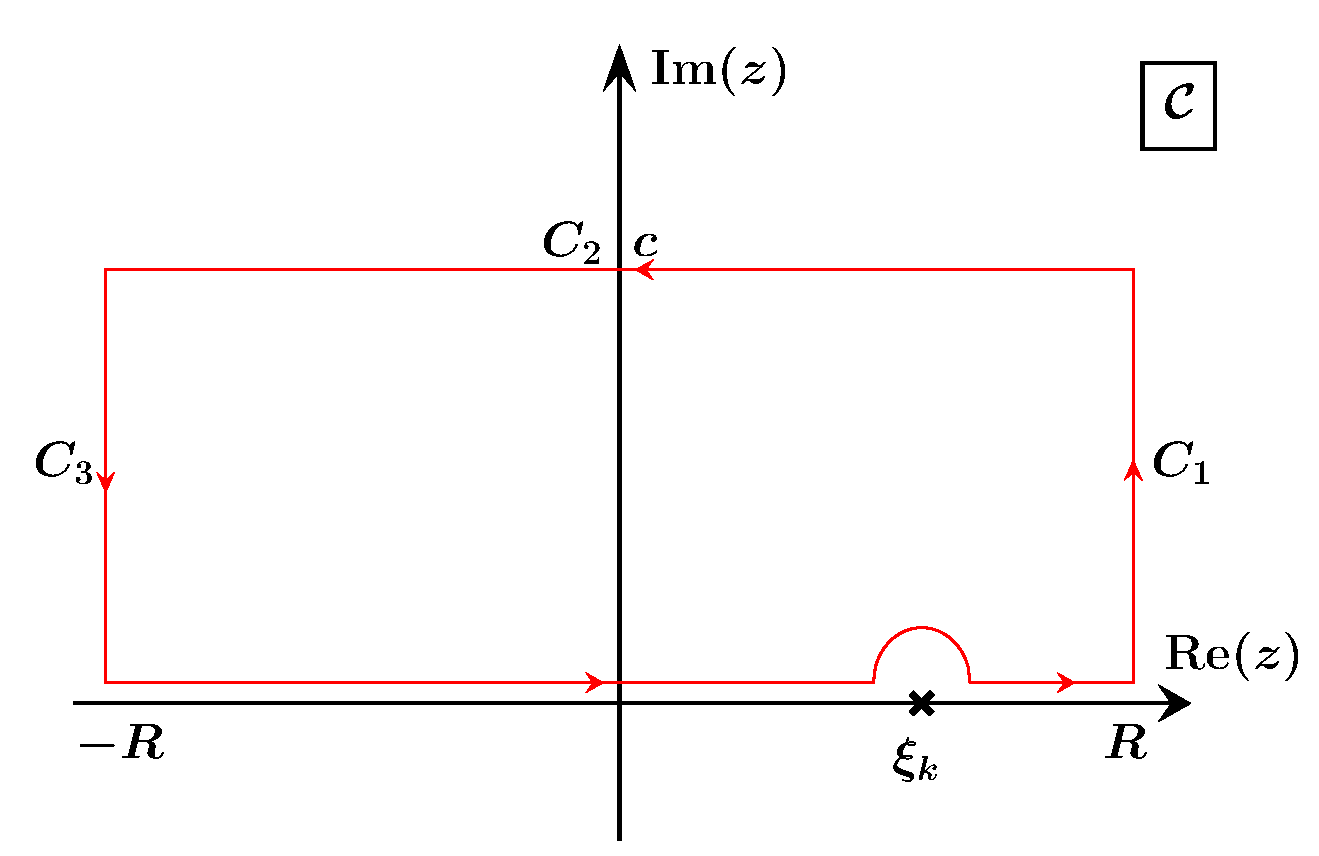
\includegraphics[width=0.7\textwidth]{plots/OgataDomain.pdf}
    \caption{Integration contour $\mathcal{C}$ of
      Eq.~(\ref{eq:OgataDomain}).\label{fig:OgataDomain}}
  \end{centering}
\end{figure}
One thus finds:
\begin{equation}
  \int_{\mathcal{C}}
  \frac{dx\,|x| (J_0(x)+iY_0(x))}{x-\xi_k} = \pi |\xi_k|
  Y_0(\xi_k)+{\rm PV} \int_{-\infty}^{\infty} \frac{dx\,|x| (J_0(x)+iY_0(x))}{x-\xi_k}=0\,,
\end{equation}
Since we are only interested in the real part of the last
integral\footnote{One should in principle prove that the imaginary
  part vanishes but, as in Ref.~\cite{Ogata:quadrature}, we will not
  do it.} and since the integrand of the real part is regular at
$x=\xi_k$, we can get rid of the principal value prescription, thus
obtaining:
\begin{equation}
\mathcal{J}_k= - \pi |\xi_k| Y_0(\xi_k)\,,
\end{equation}
that finally produces:
\begin{equation}
  \mathcal{I} = \sum_{k=-\infty \atop k\neq 0}^{\infty}\frac{\pi Y_0(\xi_k)}{J_1(\xi_k)} |\xi_k| f(\xi_k)\,.
\end{equation}
The integral in Eq.~(\ref{eq:TestIntegral}) can be rescaled by making
a change of variable $x\rightarrow h x$ where $h$ is a positive real
number, so that:
\begin{equation}
  \mathcal{I} = h\int_{-\infty}^{\infty} dx\,|hx|f(hx) =
  \pi h\sum_{k=-\infty \atop k\neq 0}^{\infty}\frac{ Y_0(\xi_k)}{J_1(\xi_k)}|h\xi_k| f(h\xi_k)\,,
\label{eq:TestIntegral}
\end{equation}
which reproduces the result of Ref.~\cite{Ogata:quadrature} when
$\nu=0$.

Now let us consider the specific integral in
Eq.~(\ref{eq:OgataQuadMast}) with $\nu=0$:
\begin{equation}
\mathcal{I}_0(q_T)=
\frac1{q_T}\int_0^\infty d\bar{b} J_0(\bar{b})
f\left(\frac{\bar{b}}{q_T}\right)\,.
\end{equation}
If we make the change of variable:
\begin{equation}
  \bar{b}=\frac{\pi}{h}\psi\left(\frac{t}{\pi}\right)\,,
  \label{eq:OgataChangeOfVariable}
\end{equation}
with $\psi$ given
in Eq.~(\ref{eq:PsiChangeOfVariable}), we obtain:
\begin{equation}
\begin{array}{rcl}
  \mathcal{I}_0(q_T)&=&\displaystyle 
              \frac1{q_T}\frac{1}{h}\int_0^\infty dt\, \psi'\left(\frac{t}{\pi}\right)  J_0\left(\frac{\pi}{h}\psi\left(\frac{t}{\pi}\right)\right)
              f\left(\frac{1}{q_T}\frac{\pi}{h}\psi\left(\frac{t}{\pi}\right)\right)\\
  \\
          &=&\displaystyle\frac{\pi}{q_T} \sum_{k=1}^{\infty}\frac{ Y_0(\xi_k)}{J_1(\xi_k)}\psi'\left(\frac{h\xi_k}{\pi}\right)  J_0\left(\frac{\pi}{h}\psi\left(\frac{h\xi_k}{\pi}\right)\right)
              f\left(\frac{1}{q_T}\frac{\pi}{h}\psi\left(\frac{h\xi_k}{\pi}\right)\right)\,,
\end{array}
\label{eq:OgataSumSingle}
\end{equation}
that finally agrees with Eq.~(\ref{eq:OgataQuadMast}). Note that,
since the integral in between zero and infinity, we limited the series
in $k$ only to positive values. It is important to notice that the
function $\psi$ has been chosen such that:
\begin{equation}
\frac{\pi}{h}\psi\left(\frac{h\xi_k}{\pi}\right)\mathop{\longrightarrow}_{k\rightarrow
\infty}\xi_k\,,
\end{equation}
so that the presence of $J_0$ suppresses contributions with large
values of $k$ thus allowing to truncate the series.

As an application of Eq.~(\ref{eq:OgataSumSingle}), we consider the
integral:
\begin{equation}
\int_0^{\infty} db\,bJ_0(b)e^{-\frac{b^2}{2}} = e^{-\frac12}\,.
\label{eq:OgataTransformSingle}
\end{equation}
In Fig.~\ref{fig:OgataTransformSingle}, the relative accuracy between
the l.h.s. of Eq.~(\ref{eq:OgataTransformSingle}) computed using
Eq.~(\ref{eq:OgataSumSingle}) truncated to the $N$-th term and with
$h=10^{-3} $ and its true value given on the r.h.s. is plotted as a
function of $N$. It is clear that the series quickly converges to its
true value as $N$ increases.
\begin{figure}[t]
  \begin{centering}
    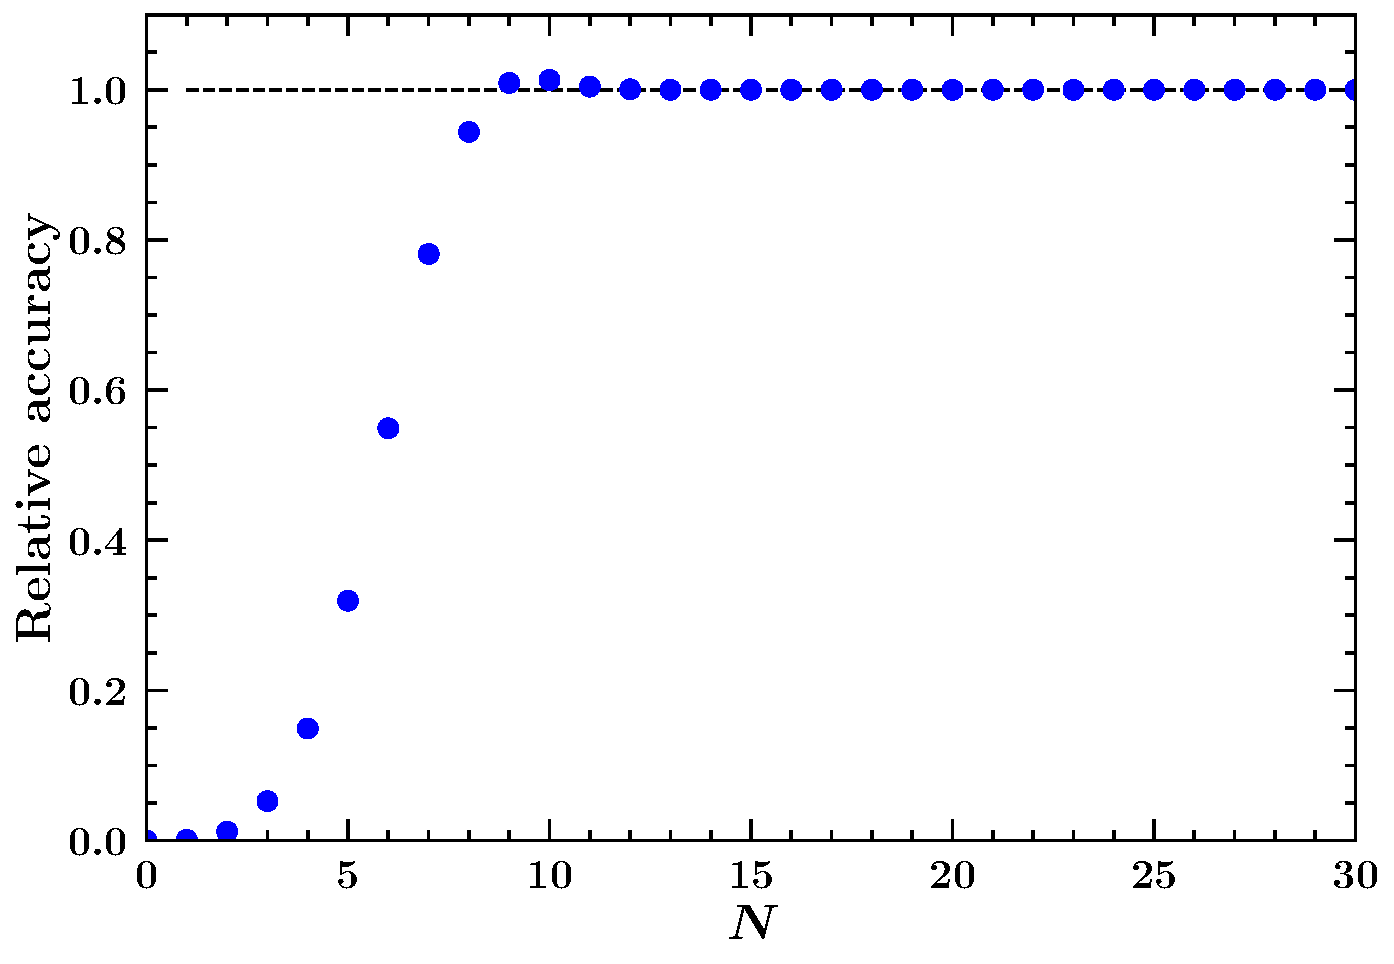
\includegraphics[width=0.6\textwidth]{plots/OgataTransformSingle.pdf}
    \caption{Relative accuracy of the integral in the l.h.s. of
      Eq.~(\ref{eq:OgataTransformSingle}) computed by means of
      Eq.~(\ref{eq:OgataSumSingle}) truncated to the $N$-th
      term.\label{fig:OgataTransformSingle}}
  \end{centering}
\end{figure}

We now want to compute a generalisation of the integrals considered
so far. Specifically:
\begin{equation}
  \mathcal{K}_0(h_{0T},h_{1T},h_{2T})=\int_0^\infty db\,b J_0(h_{T0}b) J_0(h_{1T}b) J_0(h_{2T}b)f(b) =
  \frac{1}{h_{T0}} \int_0^\infty d\overline{b}\, J_0(\overline{b})
  J_0(a_1\overline{b})
  J_0(a_2\overline{b})f\left(\frac{\overline{b}}{h_{T0}}\right)\,,
\label{eq:ThreeBesselIntegral}
\end{equation}
where $a_i=h_{Ti}/h_{T0}$. The difference
w.r.t. Eq.~(\ref{eq:OgataQuadMast}) is the fact that now the integrand
contains three, rather than one, Bessel functions generally out of
phase (\textit{i.e.} $a_i\neq 1$). Integrals of this kind, that emerge
when attempting to parameterise TMDs in transverse-momentum space
rather than in impact-parameter space, are particularly nasty to
evaluate numerically. Indeed, the combination of three Bessel
functions out of phase gives rise to a highly ``chaotic'' oscillating
behaviour that makes a brute-force computation very inefficient:
Fig.~(\ref{fig:BesselProduct}) shows one such product.
\begin{figure}[t]
  \begin{centering}
    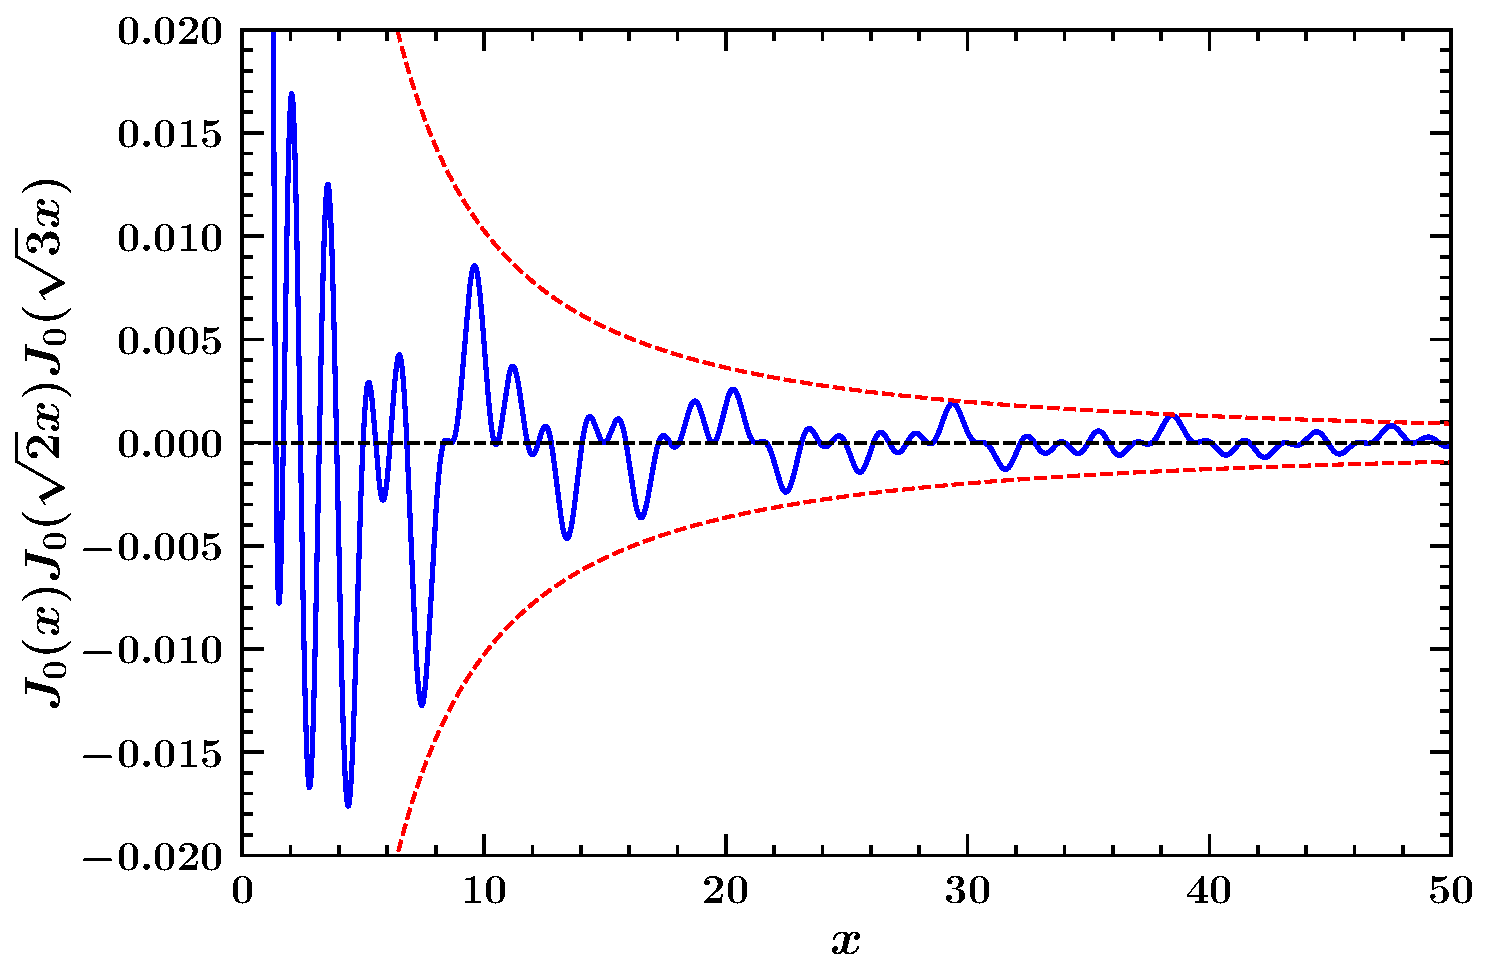
\includegraphics[width=0.6\textwidth]{plots/BesselProduct.pdf}
    \caption{Behaviour of the product of three Bessel functions out of
      phase.\label{fig:BesselProduct}}
  \end{centering}
\end{figure}

Therefore, we need to develop an \textit{ad hoc} quadrature method
aimed at making the computation of the integral in
Eq.~(\ref{eq:ThreeBesselIntegral}) efficient. To do so, we follow the
step taken by Ogata in Ref.~\cite{Ogata:quadrature} by generalising
his arguments. As in that case, the starting formula to develop a
quadrature integration is the Lagrange interpolation formula in
Eq.~(\ref{eq:LagrangeInterpolation}), but this time the function $W$
is the product of three Bessel functions rather than a single Bessel
function. If for the moment we assume that $a_1,a_2,a_1/a_2 \neq 1$,
we are guaranteed that there are no overlapping zero's of the three
$J_0$, \footnote{Actually, one should require that no zero's overlap,
  that amounts to requiring $a_1,a_2,a_1/a_2 \neq \xi_k/\xi_j$,
  $\forall\,i,j$. But configurations that violate this constraint are
  highly unlikely, except when $k=j$, that is when
  $a_1,a_2,a_1/a_2 = 1$.} we have that:
\begin{equation}
  W(x) = J_0(x)J_0(a_1x) J_0(a_2x)=\prod_{l=1}^{\infty}\left(1-\frac{x^2}{\overline{\xi}_l}\right)\,,
\end{equation}
where $\{\overline{\xi}_l\}$ is the union of the zero's of $J_0(x)$,
$J_0(a_1x)$, and $J_0(a_2x)$ that, given the assumption above, never
overlap. The computation of the derivative of $W$ computed in the node
$\overline{\xi}_k$ is easily computed:
\begin{equation}
W'(\overline{\xi}_k)=\left\{
\begin{array}{ll}
- J_1(\overline{\xi}_k)J_0(a_1\overline{\xi}_k) J_0(a_2\overline{\xi}_k)& \quad \overline{\xi}_k\mbox{ iz a zero of } J_0(x)\,,\\
- a_1J_0(\overline{\xi}_k)J_1(a_1\overline{\xi}_k) J_0(a_2\overline{\xi}_k)& \quad \overline{\xi}_k\mbox{ iz a zero of } J_0(a_1x)\,,\\
- a_2J_0(\overline{\xi}_k)J_0(a_1\overline{\xi}_k) J_1(a_2\overline{\xi}_k)& \quad \overline{\xi}_k\mbox{ iz a zero of } J_0(a_2x)\,.
\end{array}
\right.
\end{equation}
This allows us to write:
\begin{equation}
\begin{array}{rcl}
f(x)&=&\displaystyle -\sum_{\overline{\xi}_k\in\{\xi_l\}}
        f(\overline{\xi}_k)\frac{J_0(x)J_0(a_1x)
        J_0(a_2x)}{J_1(\overline{\xi}_k)J_0(a_1 \overline{\xi}_k)
        J_0(a_2 \overline{\xi}_k) (x-\overline{\xi}_k)}\\
\\
&&\displaystyle -\sum_{\overline{\xi}_k\in\{\xi_l/a_1\}}
        f(\overline{\xi}_k)\frac{J_0(x)J_0(a_1x)
        J_0(a_2x)}{a_1J_0(\overline{\xi}_k)J_1(a_1 \overline{\xi}_k)
        J_0(a_2 \overline{\xi}_k) (x-\overline{\xi}_k)}\\
\\
&&\displaystyle -\sum_{\overline{\xi}_k\in\{\xi_l/a_2\}}
        f(\overline{\xi}_k)\frac{J_0(x)J_0(a_1x)
        J_0(a_2x)}{a_2J_0(\overline{\xi}_k)J_0(a_1 \overline{\xi}_k)
        J_1(a_2 \overline{\xi}_k) (x-\overline{\xi}_k)}\,,
\end{array}
\end{equation}
where $\{\xi_l\}$ is the set of zero's of $J_0(x)$, that can be
rewritten as:
\begin{equation}
\begin{array}{rcl}
f(x)&=&\displaystyle -\sum_{k=-\infty \atop k\neq 0}^\infty
        f(\xi_k)\frac{J_0(x)J_0(a_1x)
        J_0(a_2x)}{J_1(\xi_k)J_0(a_1 \xi_k)
        J_0(a_2 \xi_k) (x-\xi_k)}\\
\\
&&\displaystyle -\sum_{k=-\infty \atop k\neq 0}^\infty
        f(\xi_k/a_1)\frac{J_0(x)J_0(a_1x)
        J_0(a_2x)}{a_1J_0(\xi_k/a_1)J_1(\xi_k)
        J_0(a_2 \xi_k/a_1) (x-\xi_k/a_1)}\\
\\
&&\displaystyle -\sum_{k=-\infty \atop k\neq 0}^\infty
        f(\xi_k/a_2)\frac{J_0(x)J_0(a_1x)
        J_0(a_2x)}{a_2J_0(\xi_k/a_2)J_0(a_1 \xi_k/a_2)
        J_1(\xi_k) (x-\xi_k/a_2)}\,.
\end{array}
\label{eq:TripleBesselInterpolation}
\end{equation}
The resulting quadrature integral is:
\begin{equation}
\begin{array}{rcl}
\displaystyle \int_{-\infty}^{\infty}dx\,|x|f(x)&=&\displaystyle -\sum_{k=-\infty \atop k\neq 0}^\infty
        \frac{|\xi_k|f(\xi_k)}{J_1(\xi_k)J_0(a_1 \xi_k)
        J_0(a_2 \xi_k) }\frac{1}{\xi_k}\int_{-\infty}^{\infty}\frac{dy\,|y| J_0(a_1y)
        J_0(a_2y)J_0(y)}{y-\xi_k}\\
\\
&&\displaystyle -\sum_{k=-\infty \atop k\neq 0}^\infty
        \frac{|\xi_k/a_1|f(\xi_k/a_1)}{a_1J_0(\xi_k/a_1)J_1(\xi_k)
        J_0(a_2 \xi_k/a_1) }\frac{1}{\xi_k}\int_{-\infty}^{\infty}\frac{dy\,|y| J_0(y/a_1)
        J_0(a_2y/a_1) J_0(y)}{y-\xi_k}\\
\\
&&\displaystyle -\sum_{k=-\infty \atop k\neq 0}^\infty
        \frac{|\xi_k/a_2| f(\xi_k/a_2)}{a_2J_0(\xi_k/a_2)J_0(a_1 \xi_k/a_2)
        J_1(\xi_k) }\frac{1}{\xi_k}\int_{-\infty}^{\infty}\frac{dy\,|y| J_0(y/a_2)J_0(a_1y/a_2)
        J_0(y)}{y-\xi_k}\,.
\end{array}
\label{eq:QuadratureIntegral}
\end{equation}
Therefore, we need to compute integrals of the following kind:
\begin{equation}
\mathcal{L}_k(c_1,c_2)=-\frac{1}{\xi_k}\int_{-\infty}^{\infty}\frac{dy\,|y| J_0(c_1y)
  J_0(c_2y)J_0(y)}{y-\xi_k}\,,
\label{eq:InterpolationWeights}
\end{equation}
where $c_1$ and $c_2$ are such that $J_0(c_i\xi_k)\neq 0$ $\forall
k$. The solution proceeds similarly as above but we need to consider
slightly more complicated contour integrals. In order to understand
better the subtleties behind the computation of these integrals, we
start from a case with two bessel functions:
\begin{equation}
  \int_{-\infty}^{\infty}\frac{dy\,|y| J_0(ay) J_0(by)}{y-t}\,,
\end{equation}
where $a$ and $b$ are two positive numbers and $t$ is a real number
that does not need to be equal to a zero of $J_0(x)$. As above, we
consider the contour integral:
\begin{equation}
  \int_{\mathcal{C}}
  \frac{dy\,|y|J_0(a y) H_0^{(1)}(by)}{y-t}\,,
\end{equation}
where $H_0^{(1)}(y) = J_0(y)+iY_0(y)$ is the Hankel function and
$\mathcal{C}$ is the same contour as in
Fig.~\ref{fig:OgataDomain}. The subtlety here is to guarantee that the
contribution from $C_2$ vanishes. To do so, we consider the asymptotic
behavior of $H_0^{(1)}$ and $J_0$ for complex numbers with large
absolute value. The relevant formulas here are:
\begin{equation}
  \begin{array}{l}
    \displaystyle |H_0^{(1)}(z)|=\sqrt{\frac{2}{\pi
    |z|}}\exp(-\mbox{Im}\,z)\left(1+\mathcal{O}(|z|^{-1})\right)\,,\quad 0 \leq \mbox{arg}\, z \leq
    \pi\,,\\
    \\
    \displaystyle |J_0^{(1)}(z)|=\sqrt{\frac{2}{\pi
    |z|}}\left(\cos\,z+\exp(-\mbox{Im}\,z)\mathcal{O}(|z|^{-1})\right)=\sqrt{\frac{1}{2\pi
    |z|}}\left(\exp(\mbox{Im}\,z)+\exp(-\mbox{Im}\,z)(1+\mathcal{O}(|z|^{-1}))\right)\,,\quad 0 \leq \mbox{arg}\, z \leq
    \pi\,.
  \end{array}
\end{equation}
In order for $|J_0(ay)||H_0^{(1)}(by)|$ to vanish as $\mbox{Im}\,z$
gets large we need that $\exp((a-b) \mbox{Im}\,z)$ is suppressed,
which implies $a<b$. Under this condition, we can use the same method
that we have used fot the single-Bessel case and obtain:
\begin{equation}
  0=\int_{\mathcal{C}} \frac{dy\,|y|J_0(a y) H_0^{(1)}(by)}{y-t}=-i\pi
  |t|J_0(a t) H_0^{(1)}(bt)+\mbox{PV}\int_{-\infty}^{\infty}
  \frac{dy\,|y|J_0(a y) H_0^{(1)}(by)}{y-t}\,.
  \label{eq:TwoBesselGeneral}
\end{equation}
Now setting $b=1$, so that $a<1$, and $t=\xi_k$, and considering only
the real part of the equality above, we obtain:
\begin{equation}
  \int_{-\infty}^{\infty} \frac{dy\,|y|J_0(a y) J_0(y)}{y-\xi_k}=-\pi
  |\xi_k|J_0(a \xi_k) Y_0^{(1)}(\xi_k)\,,\quad a<1\,.
\end{equation}
If instead $a>b$, it is sufficient to exchange $a$ and $b$ in
Eq.~(\ref{eq:TwoBesselGeneral}) which, setting $b=1$ and $t=\xi_k$,
produces:
\begin{equation}
  \int_{-\infty}^{\infty} \frac{dy\,|y|J_0(a y) J_0(y)}{y-\xi_k}=0\,,\quad a>1\,.
\end{equation}
The general result is thus:
\begin{equation}
  \int_{-\infty}^{\infty} \frac{dy\,|y|J_0(a y) J_0(y)}{y-\xi_k}=-\theta(1-a)\pi
  |\xi_k|J_0(a \xi_k) Y_0^{(1)}(\xi_k)\,.
  \label{eq:DoubleBesselWeight}
\end{equation}

We can now move to the three-Bessel case which implies considering the
contour integral:
\begin{equation}
  \int_{\mathcal{C}}
  \frac{dy\,|y|J_0(a y) J_0(b y) H_0^{(1)}(cy)}{y-t}\,,
\end{equation}
whose convergence requires that $a+b<c$. Under this assumption, one
finds:
\begin{equation}
  \mbox{PV}\int_{-\infty}^{\infty}
  \frac{dy\,|y|J_0(a y) J_0(b y) J_0(cy)}{y-t}=\mbox{Re}\left[i\pi|t|J_0(a t)
  J_0(b t) H_0^{(1)}(ct)\right]\,, \quad a+b<c\,.
\end{equation}
However, other possible hierarchies can be accommodated by just
reshuffling the arguments appropriately. There are two additional
possibilities: $a+c<b$ and $b+c <a$, that produce the general result
\begin{equation}
  \begin{array}{rcl}
    \displaystyle \mbox{PV}\int_{-\infty}^{\infty}
  \frac{dy\,|y|J_0(a y) J_0(b y) J_0(cy)}{y-t}&=&\displaystyle \theta(c-a-b)\mbox{Re}\left[i\pi|t|J_0(a t)
                                                  J_0(b t) H_0^{(1)}(ct)\right]\\
    \\
    &+&\displaystyle \theta(b-a-c) \mbox{Re}\left[i\pi|t|J_0(a t)
        J_0(c t) H_0^{(1)}(bt)\right]\\
    \\
    &+&\displaystyle \theta(a-b-c) \mbox{Re}\left[i\pi|t|J_0(b t)
        J_0(c t) H_0^{(1)}(at)\right]\,.
        \end{array}
  \label{eq:ThreeBesselGeneral}
\end{equation}
Setting $a=c_1$, $b=c_2$, $c=1$, and $t=\xi_k$, we obtain:
\begin{equation}
  \begin{array}{rcl}
    \displaystyle \mathcal{L}_k(c_1,c_2)&=&\displaystyle
                                            -\theta(1-c_1-c_2)\pi J_0(c_1 \xi_k)
                                                  J_0(c_2 \xi_k)
                                            Y_0(\xi_k)+\theta(|c_1-c_2|-1)\times
                                            0\,.
        \end{array}
  \label{eq:ThreeBesselGeneral}
\end{equation}
However, this is not the whole story because we still need to cover
the region $c_1+c_2>1$.
\begin{figure}[t]
  \begin{centering}
    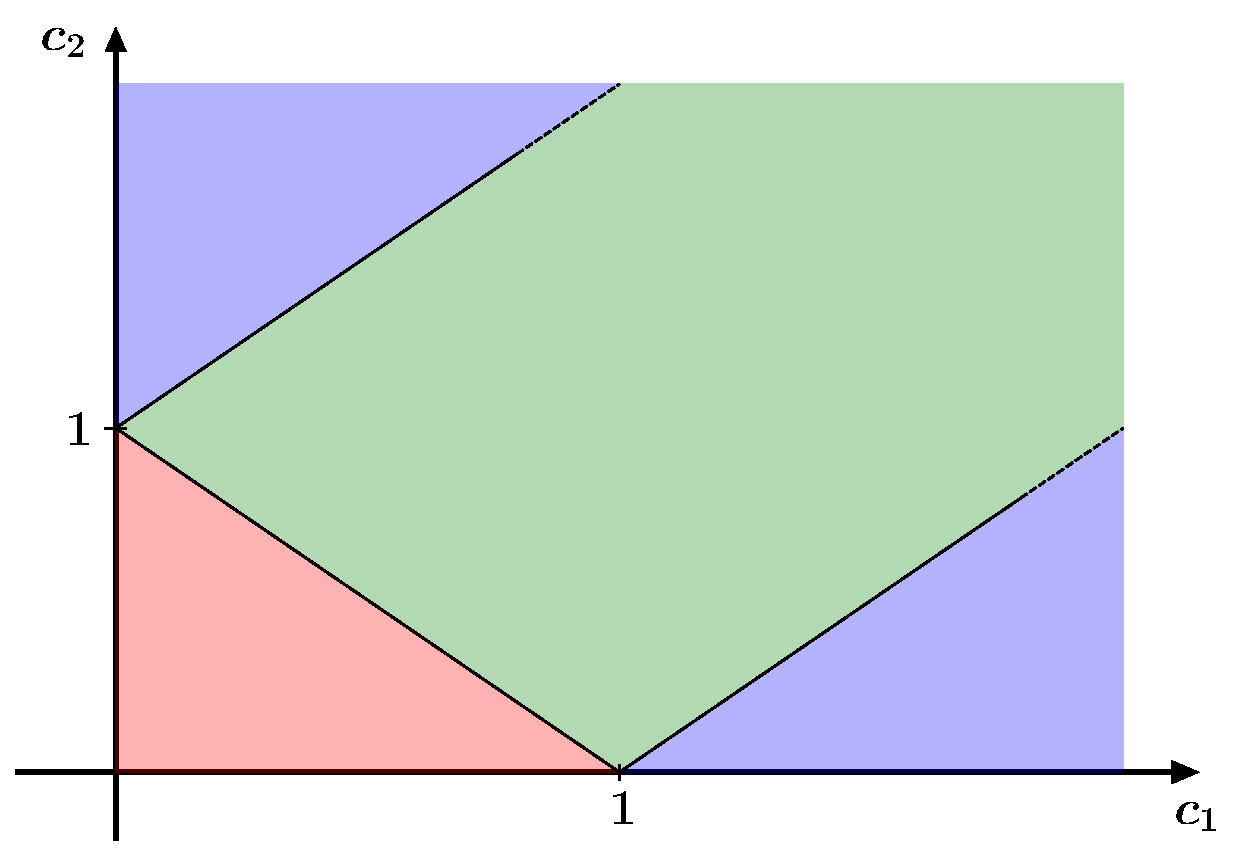
\includegraphics[width=0.7\textwidth]{plots/TripleOgataDomain.pdf}
    \caption{Domain of the interpolation weight
      $\mathcal{L}_{k}(c_1,c_2)$ in
      Eq.~(\ref{eq:InterpolationWeights}).\label{fig:TripleOgataDomain}}
  \end{centering}
\end{figure}
Referring to Fig.~\ref{fig:TripleOgataDomain}, the first term in the
r.h.s. of Eq.~(\ref{eq:ThreeBesselGeneral}) covers the red region
while the second covers the blue regions. Therefore, we still need to
cover the green region. Unfortunately, the computation in this region
is particularly cumbersome. In order to make some steps forward, we
first rewrite our target integral as follows:
\begin{equation}
  \mbox{PV}\int_{-\infty}^{\infty}\frac{dy\,|y|J_0(a y) J_0(b y)
    J_0(cy)}{y-t}= 2t \mbox{PV}\int_{0}^{\infty}\frac{dy\,yJ_0(a y)
    J_0(b y) J_0(cy)}{y^2-t^2}\,.
  \label{eq:Lc1c2Rewriting}
\end{equation}
We now consider the contour integral:
\begin{equation}
  \int_{\mathcal{P}}\frac{dy\,y H_0^{(1)}(a y) H_0^{(1)}(b y)
    J_0(cy)}{y^2-t^2} = 0\,,
  \label{eq:OgataDomainPizza}
\end{equation}
where, assuming $t>0$, $\mathcal{P}$ is the contour of the upper-right
pizza slice with infinite radius and an infinitely small semi-circle
around $t$ removed (see Fig.~\ref{fig:OgataDomainPizza}).
\begin{figure}[t]
  \begin{centering}
    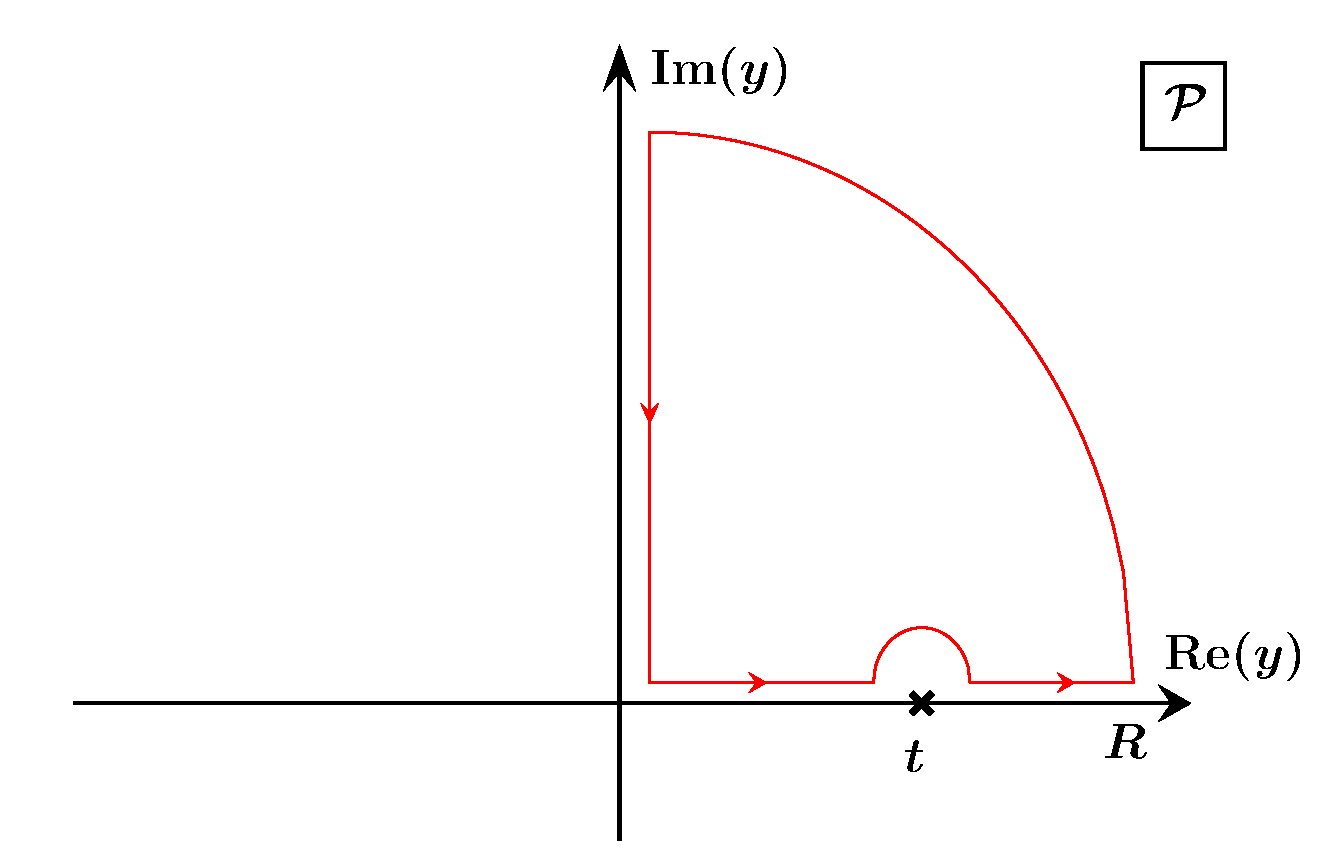
\includegraphics[width=0.8\textwidth]{plots/OgataDomainPizza.pdf}
    \caption{Integration contour $\mathcal{P}$ of
      Eq.~(\ref{eq:OgataDomainPizza}).\label{fig:OgataDomainPizza}}
  \end{centering}
\end{figure}
Since this contour contains no poles the integral must evaluate to
zero. However, In order for the integral along the quarter of circle
at infinitt to give a vanishing contribution, we need to require
$c-b-a<$. Under this requirement, we have:
\begin{equation}
  \mbox{PV}\int_{0}^{\infty}\frac{dy\,y H_0^{(1)}(a y) H_0^{(1)}(b y) J_0(cy)}{y^2-t^2}=\frac{i\pi}{2}  H_0^{(1)}(a t) H_0^{(1)}(b t) J_0(ct)-\frac{4}{\pi^2}\int_{0}^{\infty}\frac{dz\,z K_0 (az) K_0(b z) I_0(c z)}{z^2+t^2}\,,
\end{equation}
where we have used the identities $J_0(ix)=I_0(x)$ and
$H_0^{(1)}(ix)=2K_0 (x)/(i\pi)$. If we focus on the real part of this
equality and set $t=\xi_k$, we find:
\begin{equation}
  \mbox{PV}\int_{0}^{\infty}\frac{dy\,y [J_0(a y) J_0(b y)-Y_0(a y) Y_0(b y)] J_0(cy)}{y^2-\xi_k^2}=-\frac{4}{\pi^2}\int_{0}^{\infty}\frac{dz\,z K_0 (az) K_0(b z) I_0(c z)}{z^2+\xi_k^2}\,.
\end{equation}
As above, we have three independent ways of matching $a$, $b$, and $c$
with $c_1$, $c_2$, and 1. They are: 1) $a=c_1$, $b=c_2$, $c=1$ valid
for $c_2>1-c_1$, 2) $a=1$, $b=c_1$, $c=c_2$ valid for $c_2<c_1+1$, 3)
$a=c_2$, $b=1$, $c=c_1$ valid for $c_2>c_1-1$. Therefore, the overlap
region of all three combinations is precisely the green region in
Fig.~\ref{fig:TripleOgataDomain} that we are interested in. Assuming
to concentrate on this region, we have:
\begin{equation}
  \begin{array}{rcl}
    \displaystyle \mbox{PV}\int_{0}^{\infty}\frac{dy\,y [J_0(c_1 y)
    J_0( c_2y)-Y_0(c_1 y) Y_0(c_2 y)]
    J_0(y)}{y^2-\xi_k^2}&=&\displaystyle-\frac{4}{\pi^2}\int_{0}^{\infty}\frac{dz\,z
                             K_0 (c_1 z) K_0(c_2 z) I_0(
                             z)}{z^2+\xi_k^2}\,,\\
    \\
    \displaystyle   \mbox{PV}\int_{0}^{\infty}\frac{dy\,y [J_0(y)
    J_0(c_1 y)-Y_0(y) Y_0(c_1 y)]
    J_0(c_2y)}{y^2-\xi_k^2}&=&\displaystyle-\frac{\pi}{2}Y_0(\xi_k) J_0(c_1\xi_k) J_0(c_2\xi_k)
                               -\frac{4}{\pi^2}\int_{0}^{\infty}\frac{dz\,z
                               K_0 (z) K_0(c_1 z) I_0(c_2
                               z)}{z^2+\xi_k^2}\,,\\
    \\
    \displaystyle \mbox{PV}\int_{0}^{\infty}\frac{dy\,y [J_0(c_2 y)
    J_0(y)-Y_0(c_2 y) Y_0(y)] J_0(c_1y)}{y^2-\xi_k^2}&=&\displaystyle -\frac{\pi}{2}J_0(c_1\xi_k) Y_0(\xi_k) J_0(c_2\xi_k)-\frac{4}{\pi^2}\int_{0}^{\infty}\frac{dz\,z K_0 (c_2 z) K_0(z) I_0(c_1 z)}{z^2+\xi_k^2}\,.
  \end{array}
  \label{eq:ThreePossibilities}
\end{equation}
All integrals above involve our target integral, \textit{i.e.} the one
with three $J_0$. However, this integral appears entangled with other
integrals. In order to disentangle it, we consider the yet another
vanishing integral:
\begin{equation}
  \int_{\mathcal{P}}\frac{dy\,y H_0^{(1)}(a y) H_0^{(1)}(b y) H_0^{(1)}(cy)}{y^2-t^2} = 0\,,
\end{equation}
where $\mathcal{P}$ is the contour in
Fig.~\ref{fig:OgataDomainPizza}. In this case, the quarter of circle
at infinity gives a vanishing contribution for any value of $a$, $b$,
and $c$, so that:
\begin{equation}
  \mbox{PV}\int_0^{\infty}\frac{dy\,y H_0^{(1)}(a y) H_0^{(1)}(b y) H_0^{(1)}(cy)}{y^2-t^2}=\frac{i\pi}{2}H_0^{(1)}(a t) H_0^{(1)}(bt) H_0^{(1)}(ct) +\frac{8i}{\pi^3}\int_{0}^{\infty}\frac{dz\,z K_0(a z) K_0(b z) K_0(cz)}{z^2+t^2}\,.
\end{equation}
Setting as usual $t=\xi_k$, in this case there is only one independent
way to matching $a$, $b$, and $c$ with $c_1$, $c_1$ and 1, and we
choose it to be: $a=c_1$, $b=c_2$, and $c=1$. Then we focus on the
real part obtaining:
\begin{equation}
  \begin{array}{c}
  \displaystyle \mbox{PV}\int_0^{\infty}\frac{dy\,y [J_0(c_1 y)J_0(c_2 y) J_0(y) - Y_0(c_1
    y)Y_0(c_2 y) J_0(y)-Y_0(y)Y_0(c_1 y) J_0(c_2y) -Y_0(c_2y)Y_0( y) J_0(c_1y)]}{y^2-\xi_k^2}=\\
    \\
    \displaystyle -\frac{\pi}{2 }[J_0(c_1\xi_k)
    J_0(c_2 \xi_k)-Y_0(c_1\xi_k) Y_0(c_2 \xi_k)] Y_0(\xi_k)\,.
      \label{eq:OnlyPossibility}
  \end{array}
\end{equation}
Now we can sum all integrals in Eq.~(\ref{eq:ThreePossibilities}) and
subtract off the integral in Eq.~(\ref{eq:OnlyPossibility}). This
finally allows us to disentangle our target integral that yields:
\begin{equation}
  \small
  \begin{array}{rcl}
    \displaystyle \int_{-\infty}^{\infty}\frac{dy\,|y| J_0(c_1 y)
    J_0( c_2y) J_0(y)}{y^2-\xi_k^2}&=&\displaystyle-\frac{\pi}{2}|\xi_k|[J_0(c_1\xi_k)
    J_0(c_2 \xi_k)+Y_0(c_1\xi_k) Y_0(c_2 \xi_k)] Y_0(\xi_k)\\
    \\
    &-&\displaystyle \frac4{\pi^2}|\xi_k|\int_{0}^{\infty}\frac{dz\,z
                                       [K_0 (c_1 z) K_0(c_2 z)
                                       I_0(z)+K_0 (z) K_0(c_1 z)
                                       I_0(c_2z)+K_0 (c_2 z) K_0(z)
                                       I_0(c_1 z)]}{z^2+\xi_k^2}\,,
  \end{array}
\end{equation}
valid for $c_1+c_2>1\cap |c_1-c_2|<1$. The advantage of this equality
is that, while the integrand on the left-hand side is wildly
oscillating (see Fig.~\ref{fig:BesselProduct}), the integrand in the
right-hand side is exponentially suppressed in the definition region
such that a numerical evaluation is expected to be quickly convergent.
This complete the picture in that it allows us to compute the weights
$\mathcal{L}_k(c_1,c_2)$ in Eq.~(\ref{eq:InterpolationWeights}) for
any positive value of $c_1$ and $c_2$, that is:
\begin{equation}
  \small
  \mathcal{L}_k(c_1,c_2)=\left\{
  \begin{array}{ll}
    \displaystyle \pi J_0(c_1 \xi_k) J_0(c_2 \xi_k)
    Y_0(\xi_k) \,,&\quad c_1+c_2<1\,,\\
    \\
    0 \,, &\quad |c_1-c_2|>1\,,\\
    \\
    \displaystyle \frac{\pi}{2}[J_0(c_1\xi_k)
    J_0(c_2 \xi_k)+Y_0(c_1\xi_k) Y_0(c_2 \xi_k)] Y_0(\xi_k)&\\
    \\
    \displaystyle +\frac4{\pi^2}\int_{0}^{\infty}\frac{dz\,z
                                       [K_0 (c_1 z) K_0(c_2 z)
                                       I_0(z)+K_0 (z) K_0(c_1 z)
                                       I_0(c_2z)+K_0 (c_2 z) K_0(z)
                                       I_0(c_1 z)]}{z^2+\xi_k^2}\,,&\quad\mbox{otherwise.}
  \end{array}
\right.
\label{eq:ThreeBesselWeightFinal}
\end{equation}
A graphical representation of this weight as a function of $c_1$ and
$c_2$ is shown in Fig.~\ref{fig:Weight3D} for $k=1$.
\begin{figure}[t]
  \begin{centering}
    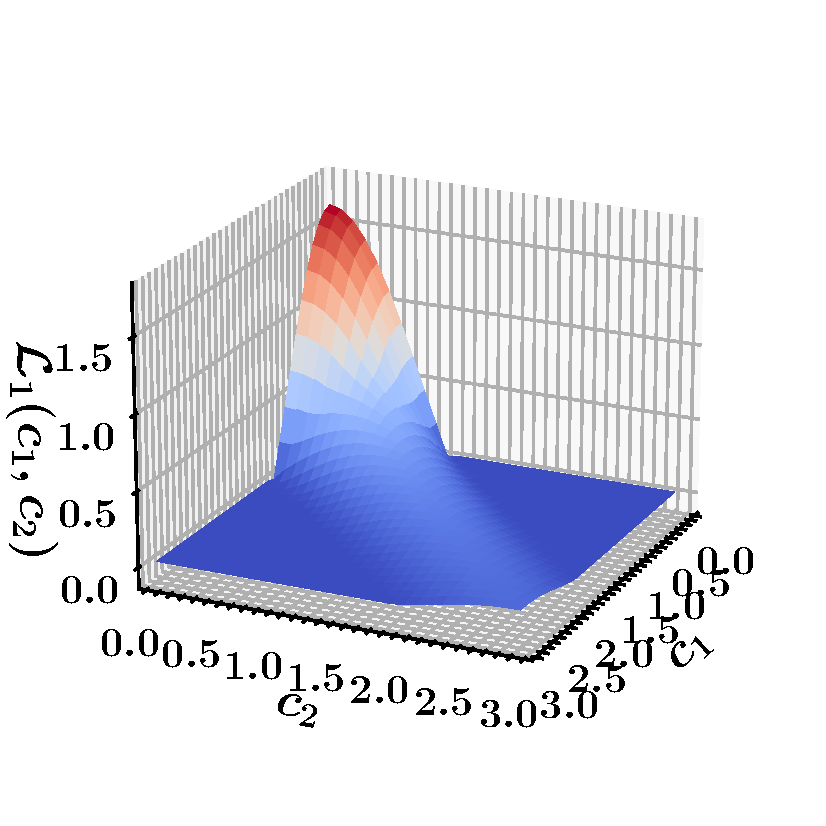
\includegraphics[width=0.7\textwidth]{plots/Weight3D.pdf}
    \caption{Graphical representation of
      Eq.~(\ref{eq:ThreeBesselWeightFinal}) with
      $k=1$.\label{fig:Weight3D}}
  \end{centering}
\end{figure}

We can now plug Eq.~(\ref{eq:ThreeBesselWeightFinal}) into
Eq.~(\ref{eq:QuadratureIntegral}). Accounting for the rescaling factor
$h$ and defining for convenience $a_0=1$, after some manipulation it
reads:
\begin{equation}
\begin{array}{rcl}
\displaystyle \int_{-\infty}^{\infty}dx\,|x|f(x)&=&\displaystyle h\sum_{k=-\infty \atop k\neq 0}^\infty |h\xi_k/a_0|f(h\xi_k/a_0)
        \frac{\theta(a_0-|a_1-a_2|)\mathcal{L}_k(a_1/a_0,a_2 /a_0)}{a_0J_1(a_0\xi_k /a_0)J_0(a_1 \xi_k/a_0)
        J_0(a_2 \xi_k /a_0) }\\
\\
&+&\displaystyle h\sum_{k=-\infty \atop k\neq 0}^\infty
        |h\xi_k/a_1|f(h\xi_k/a_1)\frac{\theta(a_1-|a_2-a_0|)\mathcal{L}_k(a_2/a_1,a_0/a_1)}{a_1 J_1(a_1\xi_k/a_1) 
        J_0(a_2 \xi_k/a_1) J_0(a_0\xi_k/a_1) }\\
\\
&+&\displaystyle h\sum_{k=-\infty \atop k\neq 0}^\infty
        |h\xi_k/a_2|f(h\xi_k/a_2)\frac{\theta(a_2-|a_0-a_1|)\mathcal{L}_k(a_0/a_2,a_1/a_2)}{a_2  J_1(a_2\xi_k/a_2) J_0(a_0\xi_k/a_2)J_0(a_1 \xi_k/a_2)}\,.
\end{array}
\label{eq:TripleSum}
\end{equation}
We have also included $\theta$-functions to limit the weights to the
region where they are different from zero. Now we define the following
list of pairs:
\begin{equation}
  \left\{\left(\overline{\xi}_i=\frac{\xi_{k(i)}}{a_{n(i)}},n(i),k(i)\right)\right\}\,,\quad
  i=-\infty,\dots,\infty\,,\quad i\neq 0
\end{equation}
in ascending order of $\overline{\xi}_i$, where $k(i)$ is the index of
the zero of $J_0$ and $n(i)\in\{0,1,2\}$. With this definition at
hand, Eq.~(\ref{eq:TripleSum}) can be written in the following compact
form:
\begin{equation}
\displaystyle \int_{-\infty}^{\infty}dx\,|x|f(x) = h\sum_{i=-\infty \atop i\neq 0}^\infty w_i|h\overline{\xi}_i|f(h\overline{\xi}_i)\,,
\end{equation}
where we have defined:
\begin{equation}
w_i=
\frac{\theta(a_{n(i)}-|a_{n(i)+1}-a_{n(i)+2}|)\mathcal{L}_{k(i)}(a_{n(i)+1}/a_{n(i)},a_{n(i)+2}
  /a_{n(i)})}{a_{n(i)}J_1(a_{n(i)}\overline{\xi}_i)J_0(a_{n(i)+1}
  \overline{\xi}_i)  J_0(a_{n(i)+2} \overline{\xi}_i) }\,,
\end{equation}
where $n(i)+1$ and $n(i)+2$ have to be interpreted as modulus 3,
\textit{i.e.} $1+2\rightarrow 0$, $2+1\rightarrow 0$, and
$2+2\rightarrow 1$.

The results above have been obtained assuming $a_1,a_2,a_1/a_2\neq
1$. We now relax these assumptions in order to include all possible
cases. In fact, one can show that this is easily accommodated by
computing the weights $w_i$ by setting $a_1=0$ if $a_1=1$, and $a_2=0$
if $a_2=1$ or if $a_2=a_1$.\footnote{In practice, in order to avoid
  divisions by zero, setting $a_1=0$ and/or $a_2=0$ really means
  setting these parameters to a small positive number.}

We can now compute the integral in
Eq.~(\ref{eq:ThreeBesselIntegral}). As above, we make the change of
variable in Eq.~(\ref{eq:OgataChangeOfVariable}) so that:
\begin{equation}
  \begin{array}{rcl}
  \mathcal{K}_0(h_{T0}, h_{T1}, h_{T2})&=&\displaystyle \frac1{h_{T0}}\frac{1}{h}\int_0^\infty dt\, \psi'\left(\frac{t}{\pi}\right)  J_0\left(\frac{\pi}{h}\psi\left(\frac{t}{\pi}\right)\right)  J_0\left(a_1\frac{\pi}{h}\psi\left(\frac{t}{\pi}\right)\right)  J_0\left(a_2\frac{\pi}{h}\psi\left(\frac{t}{\pi}\right)\right)
              f\left(\frac{1}{h_{T0}}\frac{\pi}{h}\psi\left(\frac{t}{\pi}\right)\right)\\
    \\
    &=&\displaystyle
        \frac{1}{h_{T0}}\sum_{i=1}^{\infty}w_i\psi'\left(\frac{h\overline{\xi}_i}{\pi}\right)
        J_0\left(\frac{\pi}{h}\psi\left(\frac{h\overline{\xi}_i}{\pi}\right)\right)
        J_0\left(a_1\frac{\pi}{h}\psi\left(\frac{h\overline{\xi}_i}{\pi}\right)\right)
        J_0\left(a_2\frac{\pi}{h}\psi\left(\frac{h\overline{\xi}_i}{\pi}\right)\right)
        f\left(\frac{1}{h_{T0}}\frac{\pi}{h}\psi\left(\frac{h\overline{\xi}_i}{\pi}\right)\right)\,.
  \end{array}
  \label{eq:TripleHankel}
\end{equation}
The sum in the second line is expected to converge fast to the true
value of the integral as $i$ increases. Therefore, truncating the
series at a relative small value of $i$ should provide a good
approximation of the integral. Given the symmetry of $\mathcal{K}_0$
upon reshuffling $h_{T0}$, $h_{T1}$, and $h_{T2}$, without loss of
generality one can always denote with $h_{T0}$ the largest of all such
that $a_1=h_{T1}/h_{T0}$ and $a_2=h_{T2}/h_{T0}$ are always such that
$0\leq a_i \leq 1$. This helps the convergence of the series.

To test this formula, we consider the integral:
\begin{equation}
\int_0^{\infty} db\,bJ_0(h_{T0} b)J_0(h_{T1} b)J_0(h_{T2} b)e^{-\frac{b^2}{2}}\,.
\label{eq:OgataTransformTriple}
\end{equation}
Since we do not know how to solve it exactly, in
Fig.~\ref{fig:OgataTransformTriple} we compare the convergence rate of
this integral as a function of the truncation order $N$ for different
values of $h_{T0}$, $h_{T1}$ and $h_{T2}$ computed by means of
Eq.~(\ref{eq:TripleHankel}) with
$h=10^{-2}\times\mbox{max}[h_{T0},h_{T1},h_{T2}]$ to a brute-force
numerical integration with high enough accuracy. Also in this case,
the integral converges quickly to the true value within a few terms.
\begin{figure}[t]
  \begin{centering}
    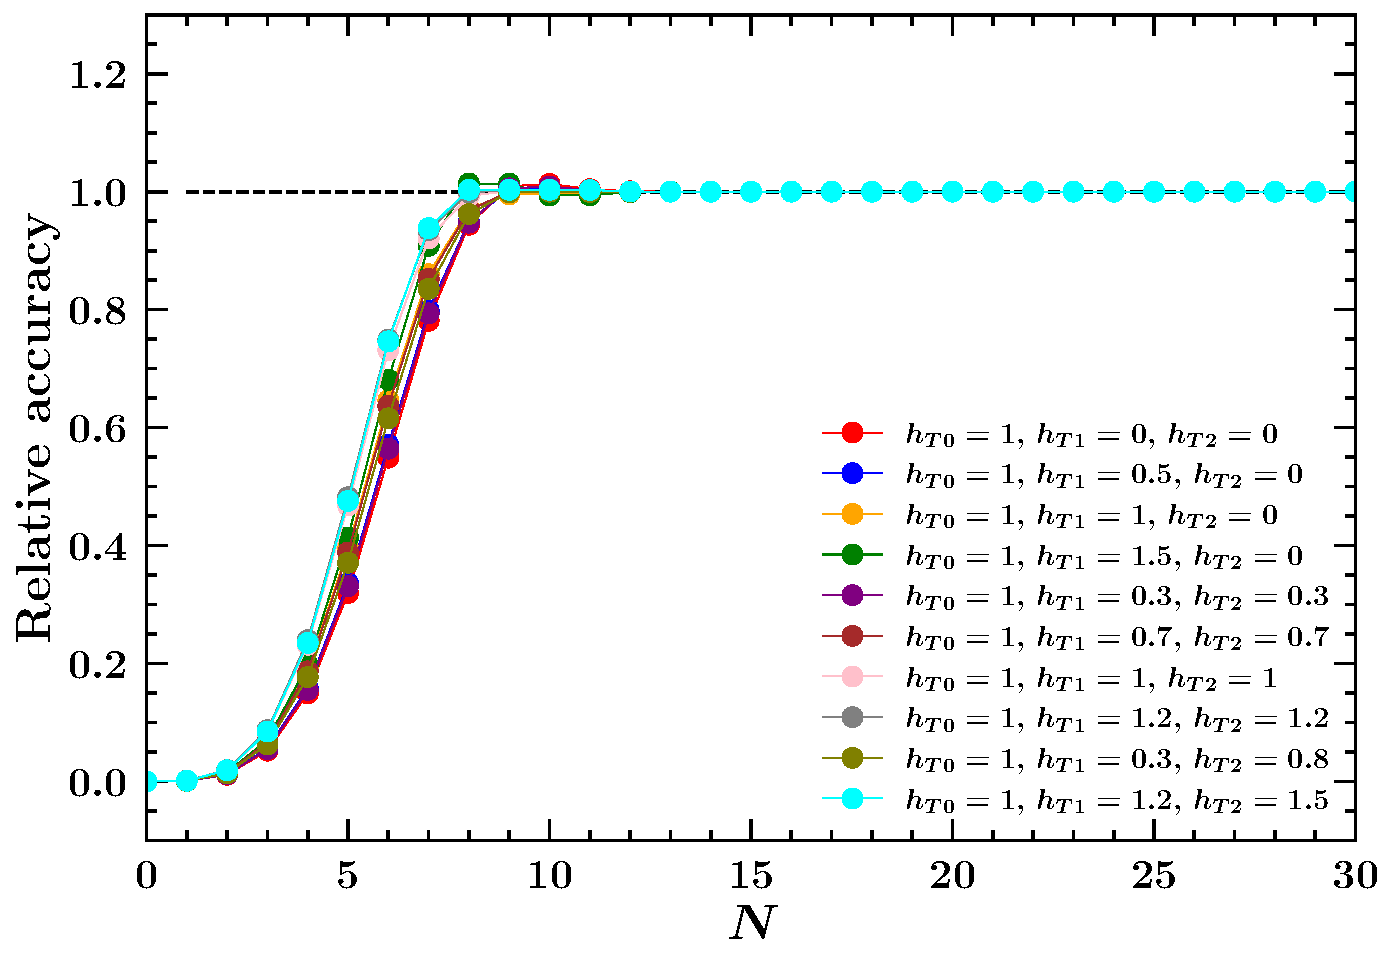
\includegraphics[width=0.6\textwidth]{plots/OgataTransformTriple.pdf}
    \caption{Relative accuracy of the integral in
      Eq.~(\ref{eq:OgataTransformTriple}) computed by means of
      Eq.~(\ref{eq:TripleHankel}) truncated to the $N$-th
      term.\label{fig:OgataTransformTriple}}
  \end{centering}
\end{figure}


\newpage
\section{Cuts on the final-state leptons}

In this section we derive explicitly the phase-space reduction factor
$\mathcal{P}$ introduced in Sect.~\ref{sec:kincuts}. This factor is
defined as:
\begin{equation}\label{eq:PSredDef}
\mathcal{P}(Q,y,q_T) = \mathcal{P}(q) = \frac{\displaystyle \int_{\mbox{\footnotesize fid.
    reg.}}d^4p_1 d^4p_2 \,\delta(p_1^2) \delta(p_2^2)\theta(p_{1,0}) \theta(p_{2,0})\delta^{(4)}(p_1+p_2-q) g_{\mu\nu}L^{\mu\nu}(p_1,p_2)}{\displaystyle \int d^4p_1 d^4p_2\, \delta(p_1^2) \delta(p_2^2) \theta(p_{1,0}) \theta(p_{2,0})\delta^{(4)}(p_1+p_2-q) g_{\mu\nu}L^{\mu\nu}(p_1,p_2)}\,,
\end{equation}
where $p_1$ and $p_2$ are the four-momenta of the outgoing leptons
and $L^{\mu\nu}$ is the leptonic tensor that, assuming massless
leptons, reads:
\begin{equation}\label{eq:lepttens}
L^{\mu\nu}(p_1,p_2) = 4(p_1^{\mu}p_2^{\nu}+p_2^{\mu}p_1^{\nu}-g^{\mu\nu}p_1p_2)\,,
\end{equation}
so that:
\begin{equation}
g_{\mu\nu}L^{\mu\nu}(p_1,p_2) = -8(p_1p_2) = -4(p_1+p_2)^2\,.
\end{equation}
In the last step we have used the on-shell-ness of the leptons
($p_1^2=p_2^2=0$). The integral in the denominator of
Eq.~(\ref{eq:PSredDef}) is restricted to some \textit{fiducial
  region}. Finally, we find:
\begin{equation}\label{eq:PSredDef2}
\mathcal{P}(q) = \frac{\displaystyle \int_{\mbox{\footnotesize fid.
    reg.}}d^4p_1 d^4p_2 \,\delta(p_1^2) \delta(p_2^2) \theta(p_{1,0}) \theta(p_{2,0})\delta^{(4)}(p_1+p_2-q) (p_1+p_2)^2}{\displaystyle \int d^4p_1 d^4p_2\, \delta(p_1^2) \delta(p_2^2) \theta(p_{1,0}) \theta(p_{2,0})\delta^{(4)}(p_1+p_2-q) (p_1+p_2)^2}\,.
\end{equation}
The effect of integrating over the fiducial region can be implemented
by defining a generalised $\theta$-function, $\Phi(p_1,p_2)$, that is
equal to one inside the fiducial region and zero outside. This allows
one to integrate also the numerator of Eq.~(\ref{eq:PSredDef2}) over
the full phase-space of the two outgoing leptons:
\begin{equation}\label{eq:PSredDef3}
\mathcal{P}(q) = \frac{\displaystyle \int d^4p_1 d^4p_2 \,\delta(p_1^2) \delta(p_2^2) \theta(p_{1,0}) \theta(p_{2,0})\delta^{(4)}(p_1+p_2-q) \Phi(p_1,p_2) (p_1+p_2)^2}{\displaystyle \int d^4p_1 d^4p_2\, \delta(p_1^2) \delta(p_2^2) \theta(p_{1,0}) \theta(p_{2,0})\delta^{(4)}(p_1+p_2-q) (p_1+p_2)^2}\,.
\end{equation}
Now we can integrate over one of the outgoing momenta, say $p_2$,
exploiting the momentum-conservation $\delta$-function both in the
numerator and in the denominator. Specifically, the numerator of
Eq.~(\ref{eq:PSredDef3}) gives:
\begin{equation}
\begin{array}{c}
\displaystyle \int d^4p_1 d^4p_2\, \delta(p_1^2)
\delta(p_2^2) \theta(p_{1,0}) \theta(p_{2,0})\delta^{(4)}(p_1+p_2-q)
  \Phi(p_1,p_2) (p_1+p_2)^2 = \\
\\
\displaystyle Q^2 \int d^4p_1 \delta(p_1^2)
\delta((q-p_1)^2) \theta(p_{1,0})
  \theta(q_0-p_{1,0})\Phi(p_1,q-p_1)\,,
\end{array}
\end{equation}
and likewise in the denominator setting $\Phi(p_1,p_2)=1$. Finally,
renaming $p_1=p$, the phase-space reduction factor reads:
\begin{equation}\label{eq:PSredDef4}
  \mathcal{P}(q) = \frac{\displaystyle \int d^4p \delta(p^2) \delta((q-p)^2) \theta(p_{0})
    \theta(q_0-p_{0})  \Phi(p,q-p)}{\displaystyle \int d^4p \delta(p^2) \delta((q-p)^2) \theta(p_{0})
    \theta(q_0-p_{0})  }\,.
\end{equation}
The $\delta$-functions can now be used to constrain two of the four
components of the momentum $p$. The first, $\delta(p_2^2)$, is usually
used to set the first component of $p$, the energy, to the on-shell
value. Since the leptons are assumed to be massless, this
produces:
\begin{equation}\label{eq:phasespacemeasure}
\int d^4p\delta(p^2)\theta(p_0) = \int d^4p\delta(E^2-|\mathbf{p}|^2)\theta(E)=\int\frac{dEd^3\mathbf{p}}{2|\mathbf{p}|}\delta(E-|\mathbf{p}|)=\int\frac{d^3\mathbf{p}}{2|\mathbf{p}|}\,.
\end{equation}
Of course, the four-momentum $p$ appearing in the rest of the
integrand has to be set on shell ($E=|\mathbf{p}|$). Now we express
the three-dimensional measure $d^3\mathbf{p}$ in spherical coordinates
as:
\begin{equation}
d^3\mathbf{p} = |\mathbf{p}|^2d|\mathbf{p}|d(\cos\theta) d\phi\,.
\end{equation}
Then we make a change of variable from $(|\mathbf{p}|,\cos\theta)$ to
$(|\mathbf{p}_T|,\eta)$: the second set of variables are exactly those
on which kinematic cuts are imposed. We do so by knowing that:
\begin{equation}
\left\{
\begin{array}{l}
|\mathbf{p}| = |\mathbf{p}_T|\cosh\eta\,,\\
\cos\theta =\tanh\eta\,.
\end{array}
\right.
\end{equation}
This leads to:
\begin{equation}
\int\frac{d^3\mathbf{p}}{2 |\mathbf{p}|} = \frac12\int|\mathbf{p}|d|\mathbf{p}|d(\cos\theta) d\phi=\frac12\int|\mathbf{p}_T|d|\mathbf{p}_T|d\eta d\phi=\frac12\int d^2\mathbf{p}_T d\eta\,.
\end{equation}

Now we consider the second $\delta$-function:
\begin{equation}\label{eq:integralyeah!}
\frac12\int d^2\mathbf{p}_T d\eta\,\delta((q-p)^2)\theta(q_0-p_0)=\frac12\int_{-\infty}^\infty d\eta
\int_0^{2\pi} d\phi \int_0^\infty|\mathbf{p}_T|d|\mathbf{p}_T|\,\delta(Q^2-2p\cdot q) \theta(q_0-p_0)\,,
\end{equation}
being $q^2=Q^2$ and $p^2=0$. It is convenient to express the
four-vector $q$ in terms of $Q$, $y$, and $\mathbf{q}_T$:
\begin{equation}\label{eq:qexplicit}
q=\left(M\cosh y,\mathbf{q}_T,M\sinh y\right)\,.
\end{equation}
with $M=\sqrt{Q^2+|\mathbf{q}_T|^2}$. While:
\begin{equation}\label{eq:pexplicit}
p=\left(|\mathbf{p}_T|\cosh\eta,\mathbf{p}_T,|\mathbf{p}_T|\sinh\eta\right)\,,
\end{equation}
so that:
\begin{equation}
p\cdot q=|\mathbf{p}_T|M\left(\cosh\eta \cosh y-\sinh\eta\sinh
  y\right)-\mathbf{p}_T\cdot
\mathbf{q}_T=|\mathbf{p}_T|M\cosh\left(\eta - y\right)-\mathbf{p}_T\cdot \mathbf{q}_T\,.
\end{equation}
We can now assume that the two-dimensional vector $\mathbf{q}_T$ is
aligned with the $x$ axis so that
$\mathbf{p}_T\cdot \mathbf{q}_T =
|\mathbf{p}_T||\mathbf{q}_T|\cos\phi$(\footnote{In
  the general case in which $\mathbf{q}_T$ forms an angle $\beta$ with
  the $x$ axis, the scalar product would result in
  $|\mathbf{p}_T||\mathbf{q}_T|\cos(\phi-\beta)$. However, the angle
  $\beta$ could always be reabsorbed in a redefinition of the
  integration angle $\phi$ in
  Eq.~(\ref{eq:integralyeah!}).}). Therefore, the argument of the
$\delta$-function in Eq.~(\ref{eq:integralyeah!}) becomes:
\begin{equation}\label{eq:deltaargument}
f(|\mathbf{p}_T|,\eta,\phi) = Q^2-2 |\mathbf{p}_T|\left[M\cosh\left(\eta - y\right)-|\mathbf{q}_T|\cos\phi\right]\,.
\end{equation}
and that of the $\vartheta$-function
$M\cosh y-|\mathbf{p}_T|\cosh\eta$. It thus appears convenient to
integrate Eq.~(\ref{eq:integralyeah!}) over $|\mathbf{p}_T|$ first:
\begin{equation}\label{eq:firstintegral}
\frac12\int_0^\infty|\mathbf{p}_T|d|\mathbf{p}_T|\,\delta(Q^2-2p\cdot q) \theta(q_0-p_0)=\frac{\overline{p}_T^2}{2Q^2}\vartheta(M\cosh y-\overline{p}_T\cosh\eta)=\frac{\overline{p}_T^2}{2Q^2}\,,
\end{equation}
with(\footnote{Notice that the $\vartheta$-function has no effect. I
  have verified it numerically but I cannot see it analytically.}):
\begin{equation}\label{eq:overpT}
\overline{p}_T(\cos\phi) = \frac{Q^2}{2 \left[M\cosh\left(\eta - y\right)-|\mathbf{q}_T|\cos\phi\right]}=\frac{Q^2}{2 |\mathbf{q}_T|}\frac1{\left[\frac{M\cosh\left(\eta - y\right)}{|\mathbf{q}_T|}-\cos\phi\right]}\,.
\end{equation}
Now we turn to consider the integral in $d\phi$. To this end, the
following relations are useful:
\begin{equation}\label{eq:intoverphi}
\int_0^{2\pi}d\phi\, f(\cos\phi) = \int_{-1}^1\frac{dx}{\sqrt{1-x^2}}\left[f(x)+f(-x)\right]\,.
\end{equation}
and:
\begin{equation}\label{eq:complicatedintegral}
\int \frac{dx}{(a\pm
  x)^2\sqrt{1-x^2}}=\frac{\sqrt{1-x^2}}{(a^2-1)(x\pm
  a)}\pm\frac{a}{(a^2-1)^{3/2}}\tan^{-1}\left(\frac{1\pm ax}{\sqrt{a^2-1}\sqrt{1-x^2}}\right)\,.
\end{equation}
The last integral is such that:
\begin{equation}\label{eq:defintoverphi}
\int_{-1}^{1} \frac{dx}{(a\pm x)^2\sqrt{1-x^2}}=\frac{\pi a}{(a^2-1)^{3/2}}\,.
\end{equation}
We now use Eqs.~(\ref{eq:intoverphi})-(\ref{eq:defintoverphi}) to
compute:
\begin{equation}
\begin{array}{rcl}
&&\displaystyle
  \frac{1}{2Q^2}\int_0^{2\pi}d\phi\,[\overline{p}_T(\cos\phi)]^2 =
                                                                    \displaystyle
                                                                    \frac{Q^2}{4
                                                                    |\mathbf{q}_T|^2}\int_0^{2\pi}\frac{d\phi}{\left[\frac{M\cosh\left(\eta
                                                                    -
                                                                    y\right)}{|\mathbf{q}_T|}-\cos\phi\right]^2}\\
\\
&=&\displaystyle \frac{Q^2}{8|\mathbf{q}_T|^2}\int_{-1}^{1}\frac{dx}{\sqrt{1-x^2}}\left[\frac{1}{\left(\frac{M\cosh\left(\eta- y\right)}{|\mathbf{q}_T|}-x\right)^2}+\frac{1}{\left(\frac{M\cosh\left(\eta- y\right)}{|\mathbf{q}_T|}+x\right)^2}\right]\\
\\
&=&\displaystyle \frac{Q^2}{8}\Bigg\{\frac{|\mathbf{q}_T|^2 x\sqrt{1-x^2}}{(M ^2\cosh ^2\left(\eta- y\right)-|\mathbf{q}_T|^2)(x^2 |\mathbf{q}_T|^2-
  M ^2\cosh ^2\left(\eta- y\right))}\\
\\
&-&\displaystyle \frac{M\cosh\left(\eta-
    y\right)}{(M^2\cosh^2\left(\eta-
    y\right)-|\mathbf{q}_T|^2)^{3/2}}\Bigg[\tan^{-1}\left(\frac{|\mathbf{q}_T|-
    xM\cosh\left(\eta-y\right)}{\sqrt{(M^2\cosh^2\left(\eta-y\right)-|\mathbf{q}_T|^2)}\sqrt{1-x^2}}\right)\\
\\
&-&\displaystyle\tan^{-1}\left(\frac{|\mathbf{q}_T|+
    xM\cosh\left(\eta-y\right)}{\sqrt{(M^2\cosh^2\left(\eta-y\right)-|\mathbf{q}_T|^2)}\sqrt{1-x^2}}\right)\Bigg]\Bigg\}_{-1}^{1}\\
\\
&=&\displaystyle \frac{\pi
  Q^2M\cosh\left(\eta -
    y\right)}{4(M^2\cosh^2\left(\eta -
    y\right)-|\mathbf{q}_T|^2)^{3/2}}
\end{array}
\end{equation}
We can go further and solve also the integral in $\eta$:
\begin{equation}\label{eq:remarkableintegral}
\begin{array}{l}
  \displaystyle \int d^4p \delta(p^2) \delta((q-p)^2) \theta(p_{0})
  \theta(q_0-p_{0})=\int_{-\infty}^\infty
  d\eta\frac{\pi Q^2M\cosh(\eta-y)}{4(M^2\cosh^2(\eta-y)-|\mathbf{q}_T|^2)^{3/2}}= \\
  \\
  \displaystyle\frac{\pi }{4}\frac{Q^2}{M^2}\int_{-\infty}^\infty
  \frac{d(\sinh\eta)}{\left(\sinh^2(\eta-y)+\frac{Q^2}{M^2}\right)^{3/2}}= \frac{\pi}{4} \frac{Q^2}{M^2}\left[\frac{M^2}{Q^2}\frac{\sinh\eta}{\sqrt{\sinh^2\eta+\frac{Q^2}{M^2}}}\right]_{-\infty}^{\infty}= \frac{\pi}{2}\,.
\end{array}
\end{equation}
Remarkably, this result gives us the denominator of
Eq.~(\ref{eq:PSredDef4}). We now need to compute the numerator by
inserting the appropriate function $\Phi$. In our case, the kinematic
cuts are identical for the outgoing leptons and read:
\begin{equation}
\eta_{\rm
  min} < \eta_{1(2)} < \eta_{\rm max}\quad\mbox{and}\quad |\mathbf{p}_{T,1(2)}| > p_{T,\rm min}\,.
\end{equation}
Therefore, the function $\Phi$ factorises into two identical functions
as:
\begin{equation}
\Phi(p_1,p_2) = \Theta(p_1)\Theta(p_2)\,,
\end{equation}
with:
\begin{equation}
  \Theta(p) = \vartheta(\eta - \eta_{\rm min})\vartheta(\eta_{\rm max}-\eta) \vartheta(|\mathbf{p}_{T}| - p_{T,\rm min}) \,. 
\end{equation}
Referring to Eq.~(\ref{eq:PSredDef4}) and considering that:
\begin{equation}
q-p=\left(M\cosh y-|\mathbf{p}_T|\cosh\eta,\mathbf{q}_T-\mathbf{p}_T,M\sinh y-|\mathbf{p}_T|\sinh\eta\right)\,.
\end{equation}
we thus have:
\begin{equation}\label{eq:intdomain}
\begin{array}{ll}
&\Phi(p,q-p) = \Theta(p) \Theta(q-p)=\\
\\
&\displaystyle 
\vartheta(\eta - \eta_{\rm min}) \vartheta(\eta_{\rm max}-\eta)
  \times\\
\\
&\displaystyle \vartheta(|\mathbf{p}_{T}| - p_{T,\rm min})\times\\
\\
&\displaystyle \vartheta\left(\frac12\ln\left(\frac{M\cosh y-|\mathbf{p}_T|\cosh\eta+M\sinh y-|\mathbf{p}_T|\sinh\eta}{M\cosh y-|\mathbf{p}_T|\cosh\eta-M\sinh y+|\mathbf{p}_T|\sinh\eta}\right)-\eta_{\rm min}\right)\times\\
\\
&\displaystyle \vartheta\left(\eta_{\rm
  max}-\frac12\ln\left(\frac{M\cosh y-|\mathbf{p}_T|\cosh\eta+M\sinh
  y-|\mathbf{p}_T|\sinh\eta}{M\cosh y-|\mathbf{p}_T|\cosh\eta-M\sinh
  y+|\mathbf{p}_T|\sinh\eta}\right)\right)\times\\
\\
&\vartheta(|\mathbf{q}_{T}-\mathbf{p}_{T}| - p_{T,\rm min})=\\
\\
1):\quad&\displaystyle \vartheta(\eta-\eta_{\rm min}) \times\vartheta(\eta_{\rm max}-\eta) \times\\
\\
2):\quad&\displaystyle \vartheta(\overline{p}_T - p_{T,\rm min})\times\\
\\
3):\quad&\displaystyle 
  \vartheta\left(\frac12\ln\left(\frac{Me^y-\overline{p}_Te^\eta}{Me^{-y}-\overline{p}_Te^{-
\eta}}\right)-\eta_{\rm min}\right)\times\vartheta\left(\eta_{\rm max}-\frac12\ln\left(\frac{Me^y-\overline{p}_Te^\eta}{Me^{-y}-\overline{p}_Te^{-
\eta}}\right)\right)\times\\
\\
4):\quad&\displaystyle \vartheta(\sqrt{|\mathbf{q}_T|^2+\overline{p}_T^2-2 |\mathbf{q}_T|\overline{p}_T\cos\phi} - p_{T,\rm min})\,,
\end{array}
\end{equation}
where in the last step we have replaced $|\mathbf{p}_T|$ with
$\overline{p}_T$ defined Eq.~(\ref{eq:overpT}). Now the question is
identifying the integration domain defined by $\Phi(p,q-p)$ on the
$(\eta,\cos\phi)$-plane. Since the $\theta$-functions in
Eq.~(\ref{eq:PSredDef4}) will be used inside a double nested integral
over $x=\cos\phi$ first and $\eta$ second, it is convenient to rewrite
the function $\Phi(p,q-p)$ in Eq.~(\ref{eq:intdomain}) as follows:
\begin{equation}\label{eq:almostfinal}
\begin{array}{rcl}
\Phi(p,q-p) &=&\displaystyle \vartheta(\eta-\eta_{\rm min}) \times
\vartheta(\eta_{\rm max}-\eta) \\
\\
&\times& \vartheta(x - f^{(2)}(\eta,
                p_{T,\rm min})) \\
\\
&\times&\displaystyle
         \vartheta(f^{(3)}(\eta,\eta_{\rm min})-x) \times \vartheta(f^{(3)}(\eta,\eta_{\rm max})-x)\\
\\
&\times&\vartheta(f^{(4)}(\eta,
         p_{T,\rm min})-x)\,,
\end{array}
\end{equation}
with:
\begin{equation}\label{eq:relevantfuncs}
\begin{array}{rcl}
f^{(2)}(\eta, p_{T,\rm cut}) & = &\displaystyle \frac{2M p_{T,\rm min}\cosh(\eta-y) 
                    - Q^{2}}{2p_{T,\rm cut}
                    |\mathbf{q}_T|}\,, \\
\\
f^{(3)}(\eta,\eta_{\rm cut}) & = &\displaystyle \frac{M \cosh(\eta-y)}{|\mathbf{q}_T|
                    }-\frac{Q^{2} \left(\sinh(\eta
                                   -y)\coth(y-\eta_{\rm cut})+\cosh(\eta-y)\right)}{2|\mathbf{q}_T|  M}\,,\\
\\
f^{(4)}(\eta, p_{T,\rm cut}) & = &\displaystyle \frac{M \cosh(\eta-y)(Q^2 - 2
                    p_{T,\rm cut}^{2} + 2 |\mathbf{q}_T|^2)- Q^{2} \sqrt{M^{2} \sinh ^{2} (\eta-y) + p_{T,\rm cut}^{2} }}{2 |\mathbf{q}_T| \left(M^{2} - p_{T,\rm cut}^{2}\right)}\,.
\end{array}
\end{equation}
Considering that $-1\leq\cos\phi\leq 1$, the integration domain is
limited to this region. Therefore, Eq.~(\ref{eq:almostfinal}) can be
written in an even more convenient way as:
\begin{equation}\label{eq:final}
\begin{array}{rcl}
\Phi(p,q-p) &=& \vartheta(\eta-\eta_{\rm min})\vartheta(\eta_{\rm
  max}-\eta)  \\
\\
&\times&\vartheta(x -
  \mbox{max}[f^{(2)}(\eta,p_{T,\rm min}),-1])\\
\\
&\times&\vartheta(\mbox{min}[f^{(3)}(\eta,\eta_{\rm min}),f^{(3)}(\eta,\eta_{\rm
         max}), f^{(4)}(\eta,p_{T,\rm
         min}),1]-x)
\end{array}
\end{equation}
such that a double integral over $\eta$ and $x$ would read:
\begin{equation}
\int_{-\infty}^{\infty}d\eta\int_{-1}^{1}dx\,\Phi(p,q-p)\dots =
\int_{\eta_{\rm min}}^{\eta_{\rm
    max}}d\eta\,\vartheta(x_2(\eta)-x_1(\eta))\int_{x_1(\eta)}^{x_2(\eta)}dx\dots\,.
\end{equation}
with:
\begin{equation}
x_1(\eta) = \mbox{max}[f^{(2)}(\eta,p_{T,\rm min}),-1]
\end{equation}
and:
\begin{equation}
x_2(\eta) = \mbox{min}[f^{(3)}(\eta,\eta_{\rm min}),f^{(3)}(\eta,\eta_{\rm
         max}),f^{(4)}(\eta,p_{T,\rm
         min}),1]\,.
\end{equation}

\begin{figure}[t]
  \begin{centering}
    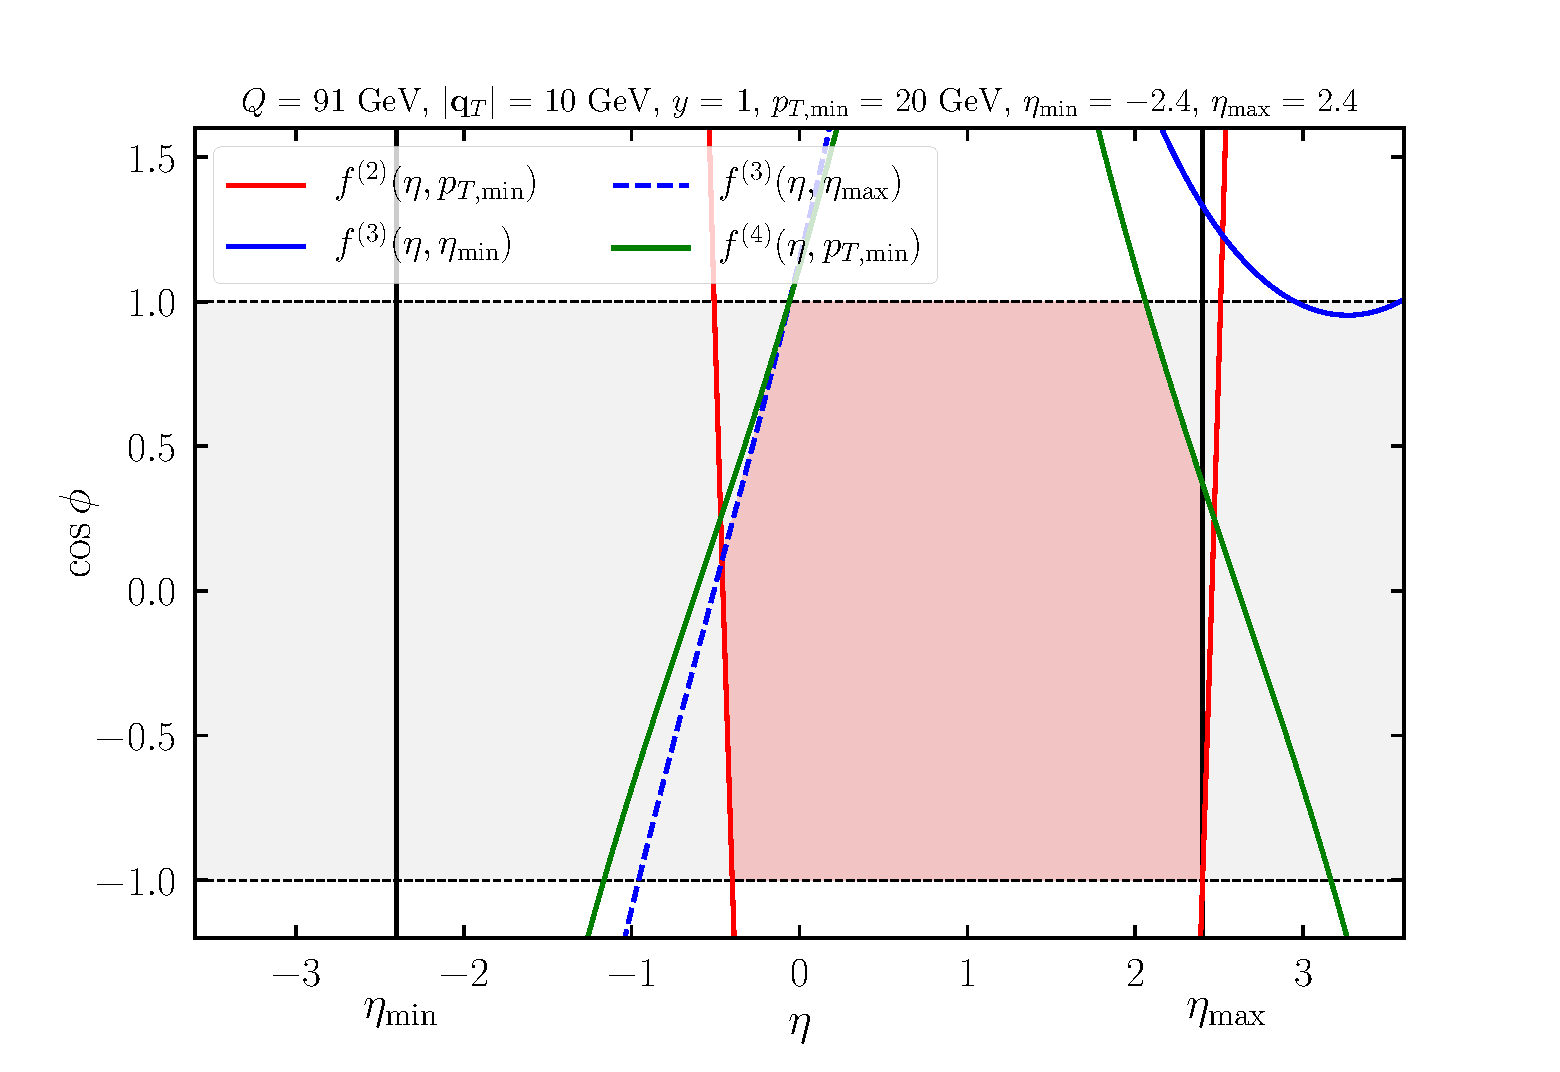
\includegraphics[width=0.8\textwidth]{plots/IntDomain.pdf}
    \caption{The red area indicates the integration domain of the
      numerator in of the phase-space reduction factor
      Eq.~(\ref{eq:PSredDef4}) for $p_{T,\rm min}=20$ GeV and
      $-\eta_{\rm min}=\eta_{\rm max}=2.4$ at $Q=91$ GeV, $|\mathbf{q}_T|=10$ GeV and
      $y=1$.\label{fig:IntDomain}}
  \end{centering}
\end{figure}
As an example, Fig.~\ref{fig:IntDomain} shows the integration domain
of the numerator in of the phase-space reduction factor
Eq.~(\ref{eq:PSredDef4}) for $p_{T,\rm min}=20$ GeV and
$-\eta_{\rm min}=\eta_{\rm max}=2.4$ at $Q=91$ GeV,
$|\mathbf{q}_T|=10$ GeV and $y=1$.  The gray band corresponds to the
region $1\leq\cos\phi\leq 1$. The $\theta$-function 1) in
Eq.~(\ref{eq:intdomain}) limits the region to the vertical stip
defined by $\eta_{\rm min} < \eta < \eta_{\rm max}$ (black vertical
lines), the $\theta$-function 2) gives the red lines, the
$\theta$-functions 3) the blue lines , and the $\theta$-function 4)
the green lines.

Gathering all pieces, the final expression for the phase-space
reduction factor reads:
\begin{equation}\label{eq:finalformula}
  \mathcal{P}(Q,y,q_T)=\displaystyle \int_{\eta_{\rm
      min}}^{\eta_{\rm
      max}}d\eta\,\vartheta(x_2(\eta)-x_1(\eta))\left[F(x_2(\eta),\eta)-F(x_1(\eta) ,\eta)\right]
\end{equation}
with:
\begin{equation}\label{eq:integrandF}
\begin{array}{rcl}
\displaystyle F(x ,\eta)&=&\displaystyle \frac{1}{4\pi}\frac{Q^2}{E_q^2-q_T^2}\Bigg\{\frac{q_T^2 x\sqrt{1-x^2}}{x^2 q_T^2-
  E_q^2}\\
\\
&-&\displaystyle \frac{E_q}{\sqrt{E_q^2-q_T^2}}\left[\tan^{-1}\left(\frac{q_T-
    xE_q}{\sqrt{E_q^2-q_T^2}\sqrt{1-x^2}}\right)-\displaystyle\tan^{-1}\left(\frac{q_T+
    xE_q}{\sqrt{E_q^2-q_T^2}\sqrt{1-x^2}}\right)\right]\Bigg\}\
\end{array}
\end{equation}
where we have defined $E_q = M\cosh(\eta-y)$ and
$q_T=|\mathbf{q}_T|$.

Let us consider the case $y=q_T=0$. For simplicity, we also take
$\eta_{\rm min} = -\eta_{\rm max}$. In these conditions,
Eq.~(\ref{eq:integrandF}) reduces to:
\begin{equation}\label{eq:F00}
F(x,\eta)=\displaystyle \frac{1}{4\pi}\frac{1}{\cosh^2(\eta)}\left[\tan^{-1}\left(\frac{
    x}{\sqrt{1-x^2}}\right)-\displaystyle\tan^{-1}\left(-\frac{
    x}{\sqrt{1-x^2}}\right)\right]\,.
\end{equation}
As evident from Eq.~(\ref{eq:relevantfuncs}), for $q_T=0$ all
functions $f^{(2)}$, $f^{(3)}$, and $f^{(4)}$ diverge. The relevant
question, though, is whether they go to plus or minus infinity
depending on the value of $Q$. Of course, $q_T$ will tend to zero
positively so we find:
\begin{equation}
\begin{array}{l}
\displaystyle f^{(2)}(\eta,p_{T,\rm min})\rightarrow \infty\times\mbox{sign}\left[2 p_{T,\rm min}\cosh(\eta)-Q\right]\,,\\
\\
\displaystyle f^{(3)}(\eta,\eta_{\rm min}= -\eta_{\rm max}) \rightarrow +\infty\\
\\
\displaystyle f^{(3)}(\eta,\eta_{\rm max}) \rightarrow -\infty\,,\\
\\
\displaystyle f^{(4)}(\eta,p_{T,\rm min}) \rightarrow \infty\times\mbox{sign}\left[\frac{\cosh(\eta)(Q^2 - 2
                    p_{T,\rm min}^{2})- Q\sqrt{Q^{2} \sinh^{2}(\eta) + p_{T,\rm min}^{2} }}{Q^{2} - p_{T,\rm min}^{2}}\right]\,, 
\end{array}
\end{equation}
Therefore, $f^{(3)}$ never actually contributes. In addition, for the
$\theta$-function in Eq.~(\ref{eq:finalformula}) to be different from
zero, we need $f^{(2)}(\eta)\rightarrow -\infty$ and
$f^{(3)}(\eta)\rightarrow \infty$. These both translate into
$Q\geq 2 p_{T,\rm min}\cosh(\eta)$. This inequality is satisfied only
if $Q\geq 2p_{T,\rm min}$ for:
\begin{equation}\label{eq:etabardef}
-\overline{\eta}\leq\eta\leq \overline{\eta}\quad\mbox{with}\quad \overline{\eta} =\cosh^{-1}\left(\frac{Q}{2p_{T,\rm min}}\right)\,.
\end{equation}
Therefore, the phase-space reduction factor eventually becomes:
\begin{equation}
\begin{array}{rcl}
  \mathcal{P}(Q,0,0)&=&\displaystyle\frac12\vartheta(Q- 2p_{T,\rm min})\displaystyle \int_{-\eta_{\rm
      max}}^{\eta_{\rm
      max}}\frac{d\eta}{\cosh^2\eta}\,\vartheta(\eta+\overline{\eta})
  \vartheta(\overline{\eta}-\eta)\\
\\
&=&\displaystyle\vartheta(Q- 2p_{T,\rm
    min})\tanh(\mbox{max}[\eta_{\rm max},\overline{\eta}])\,.
\end{array}
\end{equation}
This result can be written more explicitly as:
\begin{equation}\label{eq:partcase}
\mathcal{P}(Q,0,0) = 
\left\{
\begin{array}{ll}
0 & \quad Q< 2p_{T,\rm min}\,,\\
\displaystyle \tanh(\overline{\eta})=\left(1+\frac{2p_{T,\rm min}}{Q}\right)\sqrt{1-\frac{4 p_{T,\rm min}}{Q+2p_{T,\rm min}}}& \quad 2p_{T,\rm min} \leq Q < 2p_{T,\rm min}\cosh\eta_{\rm max}\,,\\
\tanh(\eta_{\rm max}) & \quad Q \geq 2p_{T,\rm min}\cosh\eta_{\rm max}\,.
\end{array}
\right.
\end{equation}
This differs from Eq.~(24) of Ref.~\cite{Scimemi:2017etj}. Despite the
three different regions coincide, the behavior of the phase-space
reduction factor for all regions but for $Q< 2p_{T,\rm min}$ is
different. In favour of our result there is the fact that
$\mathcal{P}(Q,0,0)$ in Eq.~(\ref{eq:partcase}) is continuous at
$Q = 2p_{T,\rm min}\cosh\eta_{\rm max}$ while that of
Ref.~\cite{Scimemi:2017etj} is not. In addition, when setting
$p_{T,\rm min} = 0$ and $\eta_{\rm max}=\infty$, \textit{i.e.} no
cuts, our result tends to $\mathcal{P}(Q,0,0)=\tanh(\infty)=1$, as it
should. While the result in Eq.~(24) of Ref.~\cite{Scimemi:2017etj}
actually diverges in this limit.

The integrand of Eq.~(\ref{eq:finalformula}), due to the behaviour of
$x_1$ and $x_2$ as functions of $\eta$, a piecewise
function. Therefore, its numerical integration is problematic in that
quadrature algorithms assume the integrand be continuos over the
integration range. The solution is to identify the discontinuity
points and integrate the function separately over the resulting
ranges. However, the complexity of the integration region
(\textit{e.g.} see Fig.~\ref{fig:IntDomain}) makes the analytical
identification of the discontinuity points very hard to achieve.

\subsection{Contracting the leptonic tensor with $g_\perp^{\mu\nu}$}

The calculation done in the previous section holds when contracting
the leptonic tensor $L_{\mu\nu}$ with the metric tensor $g^{\mu\nu}$
associated with the Lorentz structure of the hadronic tensor. However,
at small values of $|\mathbf{q}_T|$, the leading-power Lorentz
structure that one needs to multiply the leptonic tensor for is:
\begin{equation}
  g_\perp^{\mu\nu} = g^{\mu\nu}+z^\mu z^\nu-t^\mu t^\nu
  \label{eq:gmunoperp}
\end{equation}
where the vectors $z^\mu$ and $t^\mu$ in the Collins-Soper (CS) frame
are defined as:
\begin{equation}\label{eq:auxvects}
\begin{array}{l}
\displaystyle z^\mu = (\sinh y,\mathbf{0},\cosh y)\,,\\
\\
\displaystyle t^\mu = \frac{q^\mu}{Q}\,,
\end{array}
\end{equation}
and they are such that $z^2=-1$, $t^2=1$ and $zq = 0$. If we use the
on-shell-ness of $p_1$ and $p_2$ ($p_1^2=p_2^2=0$) and the momentum
conservation ($p\equiv p_1$, $p_2=q-p$), we find that
$t^\mu t^\nu L_{\mu\nu}=0$ and the quantity above reduces to:
\begin{equation}\label{eq:LT}
  L_\perp = g_\perp^{\mu\nu}L_{\mu\nu} = 4\left[\frac12q^2 + 2(zp)^2\right] = 2Q^2\left[1+4 \sinh^2(y-\eta)\frac{|\mathbf{p}_T|^2}{Q^2}\right]\,.
\end{equation}
Therefore, we need to introduce this factor in both the numerator and
the denominator of Eq.~(\ref{eq:PSredDef4}). Following the same steps
of the previous section, up to a factor $2Q^2$, this leads us to
replace the integral in Eq.~(\ref{eq:firstintegral}) with(\footnote{We
  removed the $\theta$-function as we know it does not have any
  effect.}):
\begin{equation}\label{eq:firstintegralNew}
  \frac12 \int_0^\infty|\mathbf{p}_T|\left[1+4\sinh^2(y-\eta)
  \frac{|\mathbf{p}_T|^2}{Q^2}\right]d|\mathbf{p}_T|\,\delta(Q^2-2p\cdot
  q) =\frac{2\overline{p}_T^2}{Q^2}+
  2\sinh^2(y-\eta)\frac{\overline{p}_T^4} {Q^4}\,.
\end{equation}
We can still use Eq.~(\ref{eq:complicatedintegral}) for the first term
in the r.h.s. of the equation above. For the second, instead we need
to use:
\begin{equation}\label{eq:complicatedintegral2}
\begin{array}{rcl}
\displaystyle\int \frac{dx}{(a\pm
  x)^4\sqrt{1-x^2}}&=&\displaystyle\frac{\sqrt{1-x^2}\left[(11a^2+4)x^2\pm
                       3 a(9a^2+1)x + (18a^4-5a^2+2)\right]}{6(a^2-1)^3(x\pm
  a)^3}\\
\\
&\pm&\displaystyle\frac{a(2a^2+3)}{2(a^2-1)^{7/2}}\tan^{-1}\left(\frac{1\pm
      ax}{\sqrt{a^2-1}\sqrt{1-x^2}}\right)\,,
\end{array}
\end{equation}
that is such that:
\begin{equation}
\int_{-1}^{1} \frac{dx}{(a\pm
  x)^4\sqrt{1-x^2}}=\frac{\pi a(2a^2+3)}{2(a^2-1)^{7/2}}\,.
\end{equation}
In our particular case, the integrand we are considering is the second
term in the r.h.s. term of Eq.~(\ref{eq:firstintegralNew}):
\begin{equation}\label{eq:integralmmm}
\begin{array}{l}
\displaystyle
  \frac{2\sinh^2(y-\eta)}{Q^4}\int_{-1}^{1}d(\cos\phi)\overline{p}_T^4(\cos\phi)=\\
\\
\displaystyle\frac{Q^4}{8q_T^4} \sinh^2(y-\eta) \int_{-1}^{1} \frac{dx}{\sqrt{1-x^2}}\left[\frac{1}{(a+
      x)^4}+\frac1{(a-
      x)^4}\right]= \frac{\pi Q^4}{8q_T^4}\sinh^2(y-\eta) \frac{
  a(2a^2+3)}{(a^2-1)^{7/2}}\,.
\end{array}
\end{equation}
with:
\begin{equation}
a =\frac{M}{q_T}\cosh(y-\eta)\,.
\end{equation}
Now we need to integrate Eq.~(\ref{eq:integralmmm}) over $\eta$:
\begin{equation}
  \frac{\pi Q^4}{8q_T^4} \int_{-\infty}^{\infty}d\eta\sinh^2(y-\eta)\frac{
    a(2a^2+3)}{(a^2-1)^{7/2}}\,.
\end{equation}
If we make the following change of variable in the integral above:
\begin{equation}
z=\frac{M}{q_T}\sinh(y-\eta)
\end{equation}
such that:
\begin{equation}
a^2 = z^2+\frac{M^2}{q_T^2}\quad\mbox{and}\quad dz = -ad\eta\,,
\end{equation}
the integral above becomes:
\begin{equation}
\frac{\pi Q^4}{4M^2 q_T^2} \int_{-\infty}^{\infty}dz\frac{
  z^2\left(z^2+\frac{M^2}{q_T^2}+\frac32\right)}{\left(z^2+\frac{M^2}{q_T^2}-1\right)^{7/2}}=\frac{\pi}{6}\,.
\end{equation}
Putting this result together with Eq.~(\ref{eq:remarkableintegral})
and taking into account the factor $2Q^2$ in Eq.~(\ref{eq:LT}), we find
that:
\begin{equation}\label{eq:normalisation}
\begin{array}{l}
  \displaystyle \int d^4p \delta(p^2) \delta((q-p)^2) \theta(p_{0})
  \theta(q_0-p_{0})L_\perp = \frac{4\pi}{3}Q^2\,.
\end{array}
\end{equation}
This result agrees with Eq.~(2.38) of Ref.~\cite{Scimemi:2017etj}, up
to a factor four. This provides the denominator of the
phase-space-reduction factor $\mathcal{P}$. The structure of
$\mathcal{P}$ will be exactly like that in
Eq.~(\ref{eq:finalformula}), the only thing we need to do is to
identify the correct function $F(x,\eta)$. To this end, we need to
make the following replacement for the function $F$ given in
Eq.~(\ref{eq:integrandF}) with:
\begin{equation}\label{eq:FGcombination}
F(x,\eta)\rightarrow \overline{F}(x,\eta) = \frac34 F(x,\eta)+ \frac14 G(x,\eta)\,,
\end{equation}
where:
\begin{equation}\label{eq:integrandG}
\begin{array}{rcl}
\displaystyle G(x ,\eta)&=&\displaystyle 
                            \frac{1}{16\pi }\sinh^2(y-\eta)\frac{Q^4}{(E_q^2-q_T^2)^3}
                            \Bigg\{\sqrt{1-x^2}q_T\\
\\
&\times&\displaystyle\Bigg[\frac{(11E_q^2q_T^2+4q_T^4)x^2+
                       3 E_qq_T(9E_q^2+q_T^2)x + (18E_q^4-5E_q^2q_T^2+2q_T^4)}{(xq_T+
  E_q)^3}\\
\\
&+&\displaystyle\frac{(11E_q^2q_T^2+4q_T^4)x^2-
                       3 E_qq_T(9E_q^2+q_T^2)x + (18E_q^4-5E_q^2q_T^2+2q_T^4)}{(xq_T-
  E_q)^3}\Bigg]\\
\\
&-&\displaystyle\frac{6E_q (2E_q^2+3q_T^2)}{\sqrt{E_q^2-q_T^2}}\left[\tan^{-1}\left(\frac{q_T-
      xE_q}{\sqrt{E_q^2-q_T^2}\sqrt{1-x^2}}\right)-\tan^{-1}\left(\frac{q_T+
      xE_q}{\sqrt{E_q^2-q_T^2}\sqrt{1-x^2}}\right)\right]
\Bigg\}\,.
\end{array}
\end{equation}
Finally, combining the functions $F$ and $G$ given in
Eqs.~(\ref{eq:integrandF}) and~(\ref{eq:integrandG}), respectively,
according to Eq.~(\ref{eq:FGcombination}) to obtain $\overline{F}$,
and replacing $F$ with $\overline{F}$ in Eq.~(\ref{eq:finalformula})
gives the phase-space-reduction factor $\mathcal{P}(Q,y,q_T)$ when the
leptonic tensor $L_{\mu\nu}$ is contracted with the transverse metrics
$g_\perp^{\mu\nu}$.

As a final check, it is interesting to compute $\mathcal{P}$ when
$y=q_T=0$, again assuming $\eta_{\rm min} = -\eta_{\rm max}$. In this
limit $F$ reduces to the expression in Eq.~(\ref{eq:F00}), while $G$
becomes:
\begin{equation}
\begin{array}{rcl}
\displaystyle G(x ,\eta)&=&\displaystyle 
                            \frac{3}{4\pi }\frac{\sinh^2(\eta)}{\cosh^4(\eta)}
                            \Bigg\{\left[\tan^{-1}\left(\frac{
      x}{\sqrt{1-x^2}}\right)-\tan^{-1}\left(-\frac{
      x}{\sqrt{1-x^2}}\right)\right]
\Bigg\}\,,
\end{array}
\end{equation}
such that:
\begin{equation}
\begin{array}{rcl}
  \mathcal{P}(Q,0,0)&=&\displaystyle\frac38\vartheta(Q- 2p_{T,\rm min})\displaystyle \int_{-\eta_{\rm
      max}}^{\eta_{\rm
      max}}d\eta\left[\frac{\cosh^2(\eta)+\sinh^2(\eta)}{\cosh^4(\eta)}\right]\,\vartheta(\eta+\overline{\eta})
  \vartheta(\overline{\eta}-\eta)\\
\\
&=&\displaystyle\vartheta(Q- 2p_{T,\rm
    min})\tanh(\mbox{max}[\eta_{\rm max},\overline{\eta}])\left[1-\frac{1}{4\cosh^2(\mbox{max}[\eta_{\rm max},\overline{\eta}])}\right]\,,
\end{array}
\end{equation}
with $\overline{\eta}$ defined in Eq.~(\ref{eq:etabardef}). The
relation above can be written more explicitly as:
\begin{equation}\label{eq:partcase2}
{\footnotesize
\mathcal{P}(Q,0,0) = 
\left\{
\begin{array}{ll}
0 & \quad Q< 2p_{T,\rm min}\,,\\
 \tanh(\overline{\eta})\left[1-\frac{1}{4\cosh^2(\overline{\eta})}\right]=\left(1-\frac{p_{T,\rm min}^2}{Q^2}\right)\sqrt{1-\frac{4 p_{T,\rm min}^2}{Q^2}}& \quad 2p_{T,\rm min} \leq Q < 2p_{T,\rm min}\cosh\eta_{\rm max}\,,\\
 \tanh(\eta_{\rm max})\left[1-\frac{1}{4\cosh^2(\eta_{\rm max})}\right] & \quad Q \geq 2p_{T,\rm min}\cosh\eta_{\rm max}\,.
\end{array}
\right.}
\end{equation}

The reason why we kept $\eta_{\rm min} \neq -\eta_{\rm max}$ is that
in some cases it may be required to implement an asymmetric cut,
$\eta_{\rm min}<\eta<\eta_{\rm max}$. This is the case, for example,
of the LHCb experiment that delivers data only in the forward region
($2 < \eta < 4.5$).
\begin{figure}[t]
  \begin{centering}
    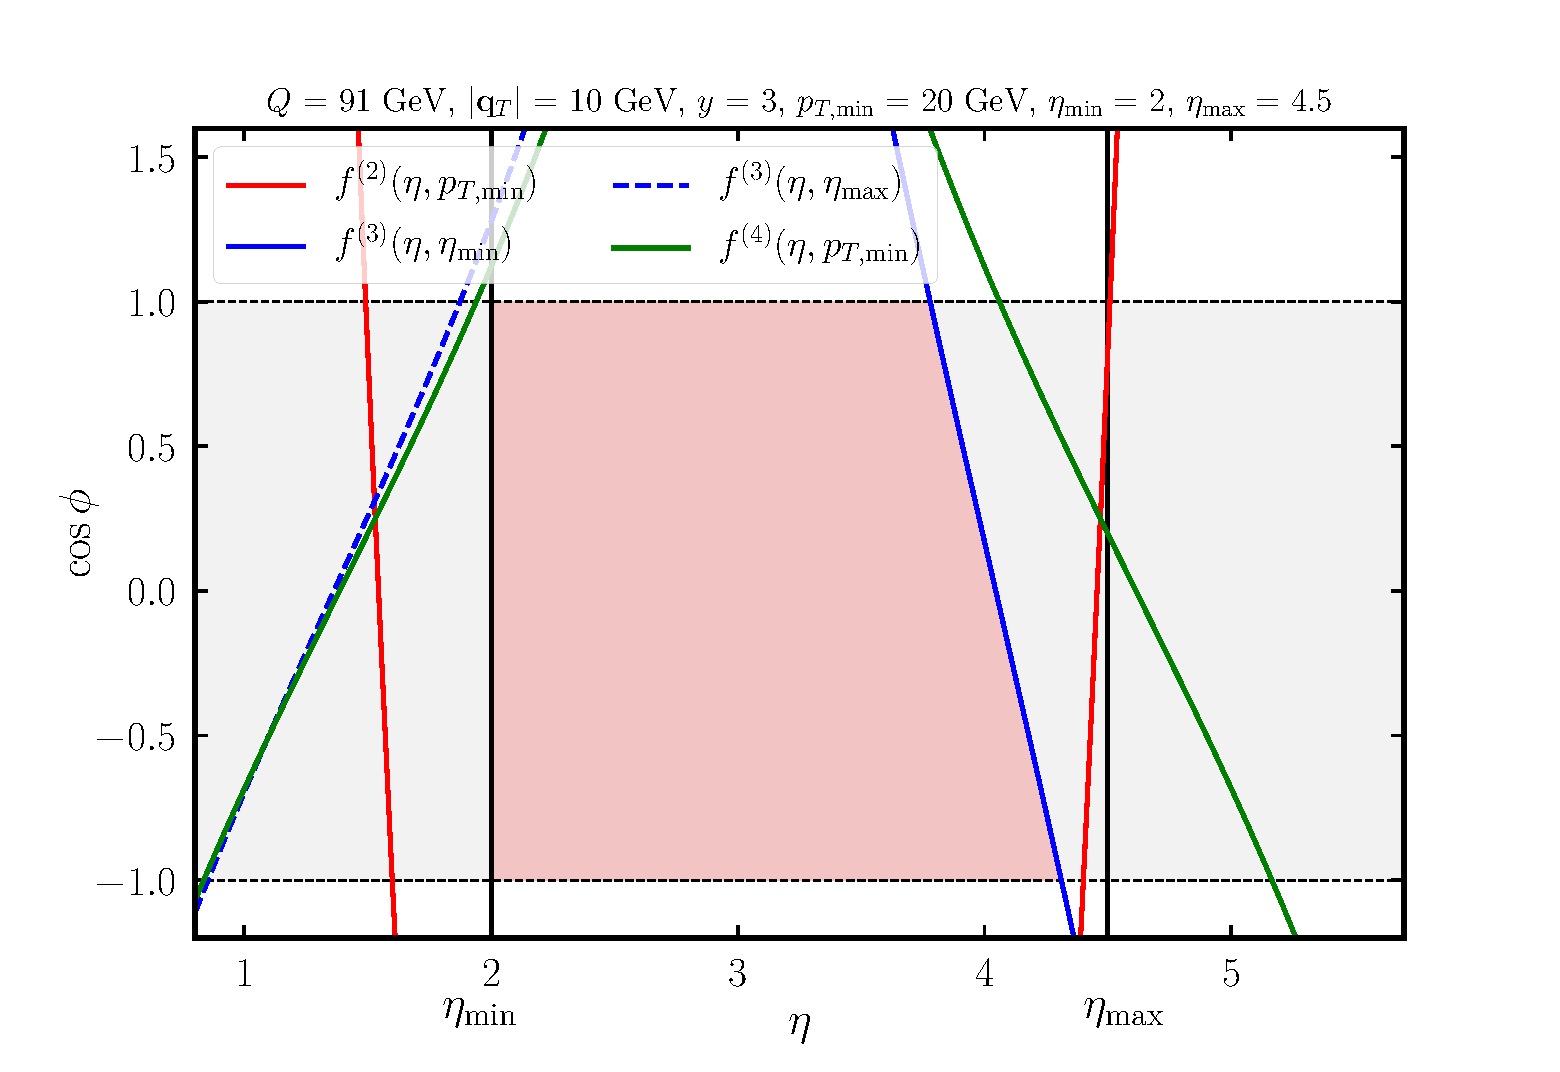
\includegraphics[width=0.8\textwidth]{plots/IntDomainAsy.pdf}
    \caption{Same as Fig.~\ref{fig:IntDomain} for the asymmetric
      rapidity cut $2<\eta < 4.5$ at $y=3$.\label{fig:IntDomainAsy}}
  \end{centering}
\end{figure}
As an example, Fig.~\ref{fig:IntDomainAsy} shows the integration
domain of the phase-space reduction factor Eq.~(\ref{eq:PSredDef4})
for $p_{T,\rm min}=20$ GeV and $2<\eta < 4.5$ at $Q=91$ GeV,
$|\mathbf{q}_T|=10$ GeV and $y=3$.

\subsection{Parity-violating contribution}

In the presence of cuts on the final-state leptons and for invariant
masses around the $Z$ mass, parity-violating effects arise. As we will
show below, these effects integrate to zero when removing the leptonic
cuts. This contribution stems from interference of the antisymmetric
contributions to the lepton tensor, proportional to $p_1^{\mu}
p_2^{\nu}\epsilon_{\mu\nu\rho\sigma}$, and the hadronic tensor,
proportional to $\epsilon_{\perp}^{\mu\nu}$ defined as:
\begin{equation}
\epsilon_{\perp}^{\mu\nu}\equiv \epsilon^{\mu\nu\rho\sigma}t_\rho z_\sigma\,,
\end{equation}
where $t^\mu$ and $z^\mu$ are given in Eq.~(\ref{eq:auxvects}).
Therefore, the contribution we are after results from the contraction
of the following Lorentz structures:
\begin{equation}
L_{\rm PV}\equiv p_1^{\mu}
p_2^{\nu}\epsilon_{\mu\nu\rho\sigma}\epsilon_{\perp}^{\rho\sigma}\,.
\end{equation}
After some manipulation, one finds:
\begin{equation}\label{eq:pvphasespace}
\begin{array}{rcl}
\displaystyle L_{\rm PV}&=& \displaystyle
p_1^{\mu}
p_2^{\nu}\epsilon_{\mu\nu\rho\sigma}\epsilon^{\rho\sigma\alpha\beta}t_\alpha
z_\beta= -2 p_1^{\mu}
p_2^{\nu}\delta_\mu^\alpha \delta_\nu^\beta t_\alpha \\
\\
&=&\displaystyle -2 (p_1 t)(p_2 z) = -2 (pt)\left[(qz)-(pz)\right] = 2(pt)(pz)\\
\\
&=&\displaystyle \frac{2|\mathbf{p}_T|^2}{Q}\sinh(y-\eta)\left[M\cosh(y-\eta)-|\mathbf{q}_T|\cos\phi\right]\,,
\end{array}
\end{equation}
where I have defined $p_1\equiv p$ and used the equalities
$p_2 = q - p$, and $zq=0$. To compute the third line I have used the
explicit parameterisation of $q$ and $p$ given in
Eqs.~(\ref{eq:qexplicit}) and~(\ref{eq:pexplicit}), respectively. The
presence of $\sinh(y-\eta)$ in Eq.~(\ref{eq:pvphasespace}) is such
that integrating over the full range in the lepton rapidity $\eta$
nullifies this contribution:
\begin{equation}\label{eq:noPVcontr}
\int_{-\infty}^{\infty} d\eta\,L_{\rm PV} = 0\,.
\end{equation}
Therefore, it turns out that, for observables inclusive in the lepton
phase space, the parity violating term does not give any
contribution. Conversely, the presence of cuts on the final-state
leptons may prevent Eq.~(\ref{eq:noPVcontr}) from being satisfied
leaving a residual contribution. In order to quantify this effect, we
take the same steps performed in the previous sections to integrate
$L_{\rm PV}$ over the fiducial region. As above, we start integrating
over the full range in $|\mathbf{p}_T|$ using the on-shell-ness
$\delta$-function:
\begin{equation}
\begin{array}{c}
\displaystyle \int_0^\infty d|\mathbf{p}_T||\mathbf{p}_T|\,L_{\rm PV}=\frac{\sinh(y-\eta)}{Q}\left[M\cosh(y-\eta)-|\mathbf{q}_T|\cos\phi\right]
\int_0^\infty d|\mathbf{p}_T||\mathbf{p}_T|^3\delta(Q^2-2pq)\\
\\
\displaystyle = \frac{\overline{p}_T^4}{Q^3}\sinh(y-\eta)\left[M\cosh(y-\eta)-|\mathbf{q}_T|\cos\phi\right]\,,
\end{array}
\end{equation}
with $\overline{p}_T$ defined in Eq.~(\ref{eq:overpT}). Now we compute
the indefinte integral over $\cos\phi$. To do so, we need to use
Eq.~(\ref{eq:intoverphi}) along with the equality:
\begin{equation}\label{eq:complicatedintegral3}
\int \frac{dx}{(a\pm
  x)^3\sqrt{1-x^2}}=\frac{\sqrt{1-x^2}\left[3ax\pm(4a^2-1) \right]}{2(a^2-1)^2(x\pm
  a)^2}\pm\displaystyle\frac{(2a^2+1)}{2(a^2-1)^{5/2}}\tan^{-1}\left(\frac{1\pm
      ax}{\sqrt{a^2-1}\sqrt{1-x^2}}\right)\,.
\end{equation}
This allows us to compute the integral(\footnote{The factor
  $\left(\frac {4\pi Q^2}{3}\right)^{-1}$ in
  Eq.~(\ref{eq:Hdefinition}) corresponds to the full phase-space in
  integral of $L_\perp$ in Eq.~(\ref{eq:normalisation}) that provides
  the natural normalisation.}):
\begin{equation}\label{eq:Hdefinition}
\begin{array}{rcl}
\displaystyle H(x,\eta)&=&\displaystyle\left(\frac {4\pi Q^2}{3}\right)^{-1}\frac{\sinh(y-\eta)}{Q^3}\left[M\cosh(y-\eta) \int
  d(\cos\phi)\overline{p}_T^4(\cos\phi)- |\mathbf{q}_T|
  \int d(\cos\phi) \cos\phi\,\overline{p}_T^4(\cos\phi)\right]\\
\\
&=&\displaystyle\frac{3Q^3 \sinh(y-\eta)}{64\pi |\mathbf{q}_T|^4}\left[M\cosh(y-\eta) \int
  \frac{d(\cos\phi)}{\left(a-\cos\phi\right)^4}-|\mathbf{q}_T|\int
  \frac{\cos\phi \,d(\cos\phi)}{\left(a-\cos\phi\right)^4}\right]\\
\\
&=&\displaystyle\frac{3Q^3 \sinh(y-\eta)}{64\pi q_T^3} \int
  \frac{dx}{\sqrt{1-x^2}}\left[\frac{1}{(a-x)^3}+\frac{1}{(a+x)^3}\right]\\
\\
&=&\displaystyle\frac{3Q^3 \sinh(y-\eta)}{128\pi q_T^3}\Bigg\{\frac{\sqrt{1-x^2}}{(a^2-1)^2}\left[\frac{3ax-(4a^2-1) }{(x-
  a)^2}+\frac{3ax+(4a^2-1) }{(x+
  a)^2}\right]\\
\\
&-&\displaystyle\frac{(2a^2+1)}{(a^2-1)^{5/2}}\left[\tan^{-1}\left(\frac{1-
      ax}{\sqrt{a^2-1}\sqrt{1-x^2}}\right) -\tan^{-1}\left(\frac{1+
      ax}{\sqrt{a^2-1}\sqrt{1-x^2}}\right)\right]\Bigg\}
\end{array}
\end{equation}
with $E_q=M\cosh\left(\eta - y\right)$, $q_T=|\mathbf{q}_T|$, and:
\begin{equation}
  a = \frac{E_q}{q_T}\,,
\end{equation}
so that:
\begin{equation}\label{eq:Hfinal}
\begin{array}{rcl}
\displaystyle H(x,\eta)&=&\displaystyle\frac{3Q^3 \sinh(y-\eta)}{128\pi (E_q^2-q_T^2)^{2}}\Bigg\{\sqrt{1-x^2}q_T\left[\frac{3E_qq_Tx-(4E_q^2-q_T^2) }{(xq_T-
  E_q)^2}+\frac{3E_qq_Tx+(4E_q^2-q_T^2) }{(q_Tx+
  E_q)^2}\right]\\
\\
&-&\displaystyle\frac{(2E_q^2+q_T^2)}{\sqrt{E_q^2-q_T^2}}\left[\tan^{-1}\left(\frac{q_T-
      xE_q}{\sqrt{E_q^2-q_T^2}\sqrt{1-x^2}}\right) -\tan^{-1}\left(\frac{q_T+
      xE_q}{\sqrt{E_q^2-q_T^2}\sqrt{1-x^2}}\right)\right]\Bigg\}\,.
\end{array}
\end{equation}
Finally, using the definition of $H$ in Eq.~(\ref{eq:Hfinal}), one can
perform the integral over the fiducial phase space as discussed
above in Eq.~(\ref{eq:finalformula}):
\begin{equation}\label{eq:finalformulaH}
  \mathcal{P}_{\rm PV}(Q,y,q_T)=\displaystyle \int_{\eta_{\rm
      min}}^{\eta_{\rm
      max}}d\eta\,\vartheta(x_2(\eta)-x_1(\eta))\left[H(x_2(\eta),\eta)-H(x_1(\eta) ,\eta)\right]\,.
\end{equation}
This allows one to estimate the impact of the parity-violating
contribution to the phase-space reduction factor.

In order to quantify numerically the impact of
Eq.~(\ref{eq:finalformulaH}), Fig.~\ref{fig:PhaseSpaceRedFactor}
displays the size $\mathcal{P}_{\rm PV}$ relative to the
parity-conserving phase-space reduction factor as a function of $y$
for three different values of $q_T$ at $Q=M_Z$ and for the following
lepton cuts: $p_{T,\ell}>20$ GeV and $-2.4 < \eta_\ell < 2.4$.
\begin{figure}[t]
  \begin{centering}
    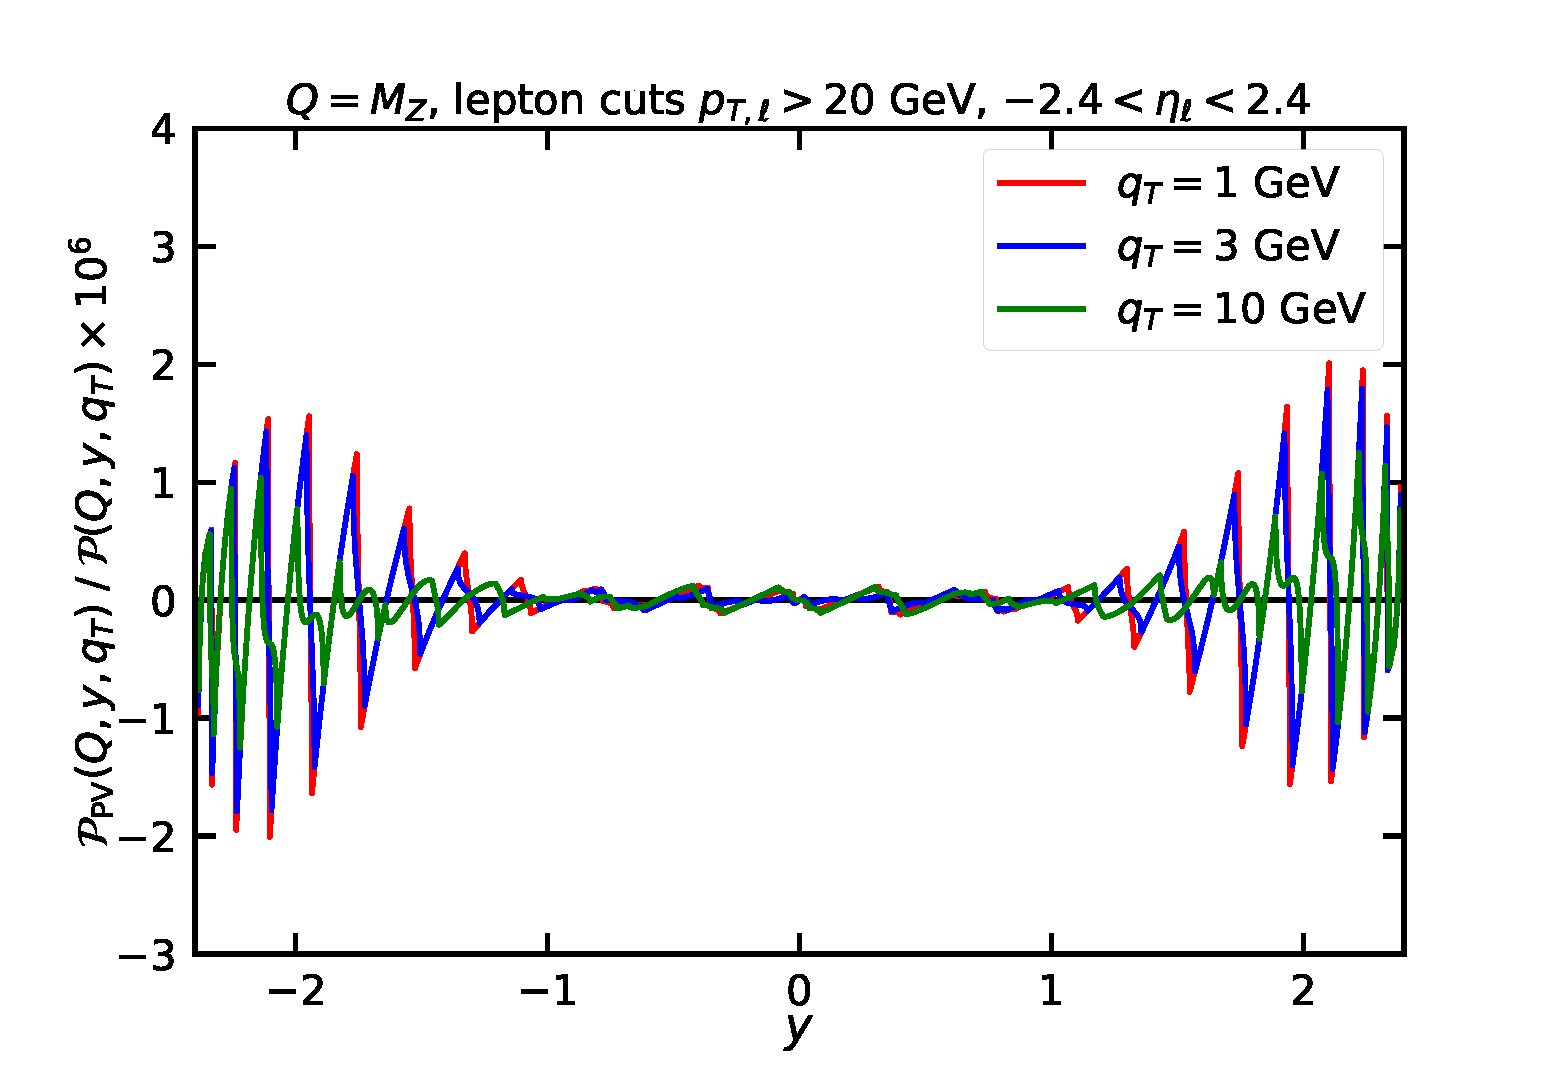
\includegraphics[width=0.8\textwidth]{plots/PhaseSpaceRedFactor.pdf}
    \caption{Ratio between the parity-violating phase-space reduction
      factor $\mathcal{P}_{\rm PV}$ in Eq.~(\ref{eq:finalformulaH})
      and the respective parity-conserving factor as a function of the
      $Z$ rapidity $y$ at $Q=M_Z$ and for three different values of
      $q_T$, with lepton cuts equal to $p_{T,\ell}>20$~GeV and
      $-2.4 < \eta_\ell < 2.4$.\label{fig:PhaseSpaceRedFactor}}
  \end{centering}
\end{figure}
It turns out that the size of $\mathcal{P}_{\rm PV}$ relative to
$\mathcal{P}$ is never larger than $2\times10^{-6}$. In addition, the
rapid oscillations with $y$ contribute to suppress even more the
integral over realistic bins in $y$. One can thus conclude that, for
realistic kinematic configurations, the impact of parity violating
effects is completely negligible.

% To conclude this section we try to compute analytically the behaviour
% of $\mathcal{P}_{\rm PV}$ in a particular kinematic configuration. For
% $q_T = y = 0$ one has that:
% \begin{equation}
% \displaystyle H(x,\eta)=-\frac{3
%                            \sinh(\eta)}{64\pi \cosh^3(\eta)}\displaystyle \left[\tan^{-1}\left(\frac{x}{\sqrt{1-x^2}}\right) -\tan^{-1}\left(\frac{-x}{\sqrt{1-x^2}}\right)\right]\,.
% \end{equation}

We finally notice that also following contraction enters the game in
the presence of cuts on the leptonic final state:
\begin{equation}
  L_\phi=(z^\mu t^\nu+z^\nu t^\mu)L_{\mu\nu}\,.
\end{equation}
We find that:
\begin{equation}
L_\phi=8(zp)\left[Q-2(tp)\right]\,.
\end{equation}
Using Eqs.~(\ref{eq:pexplicit}) and~(\ref{eq:auxvects}), we
have that:
\begin{equation}
(zp) = p_T(\cosh\eta\sinh y-\sinh\eta\cosh y) = p_T\sinh(y-\eta)\,,
\end{equation}
and:
\begin{equation}
(tp) = \frac1{Q}\left[Mp_T\cosh(y-\eta)-\mathbf{q}_T\cdot
  \mathbf{p}_T\right] = \frac{p_T}{Q}\left[M\cosh(y-\eta)-q_T\cos\phi\right]\,.
\end{equation}
Therefore:
\begin{equation}
L_\phi=16 \frac{p_T^2}{Q}\sinh(y-\eta)\left[\frac{Q^2}{2 p_T
  }-M\cosh(y-\eta)+q_T\cos\phi\right]=16\left[\frac12p_TQ\sinh(y-\eta)-L_{\rm PV}\right]\,.
\end{equation}
Due to the presence of the overall factor $\sinh(y-\eta)$, also this
contribution is expected to be subdominant.

\subsection{Asymmetric cuts}

In some circumstances, asymmetric cuts are necessary to match the
experimental measurements. More specifically, the two outgoing leptons
undergo different cuts depending on their hierarchy. Usually, one
defines the (sub)leading lepton as the lepton with the (smallest)
largest $p_T$ and according to whether the lepton is leading or
subleading a different cut on the $p_T$ is enforced. In this case, the
cut function $\Phi$ needs to be generalised as follows:
\begin{equation}
\Phi(p_1,p_2) = \vartheta(p_{T,1}^2-p_{T,2}^2)\Theta^{(1)}(p_1)
\Theta^{(2)}(p_2)+\vartheta(p_{T,2}^2-p_{T,1}^2)\Theta^{(1)}(p_2)
\Theta^{(2)}(p_1)\,,
\end{equation}
where the functions $\Theta^{(1)}$ and $\Theta^{(2)}$ are defined as:
\begin{equation}
\Theta^{(i)}(p) = \vartheta(\eta - \eta_{\rm min})\vartheta(\eta_{\rm
  max}-\eta) \vartheta(p_{T}- p_{T,\rm min}^{(i)})\,,\quad
i = 1,2\,,
\end{equation}
with $p_{T,\rm min}^{(1)}\neq p_{T,\rm min}^{(2)}$ in general. As seen
above, the lepton four-momenta $p_1$ and $p_2$ are subject to
kinematic constraints such that one effectively has $p_1=p$ and
$p_2=q-p$ with $p_{T,1}=\overline{p}_T$, with $\overline{p}_T$ defined
in Eq.~(\ref{eq:overpT}), and:
\begin{equation}
p_{T,2}^2 = q_T^2+\overline{p}_T^2-2 q_T\overline{p}_T\cos\phi\,.
\end{equation}
Therefore, the functions $\vartheta(p_{T,1}^2-p_{T,2}^2)$ and
$\vartheta(p_{T,2}^2-p_{T,1}^2)$ can be reduced to the following
$\vartheta$-functions on the azimuthal angle $\phi$:
\begin{equation}
\vartheta(p_{T,1}^2-p_{T,2}^2) =
  \vartheta\left(\cos\phi-\frac{q_T\cosh(\eta-y)}{M}\right)
  \,,\quad \vartheta(p_{T,2}^2-p_{T,1}^2) =\vartheta\left(\frac{q_T\cosh(\eta-y)}{M}-\cos\phi\right)\,.
\end{equation}
Generalising the procedure detailed above for the implementation of
the cuts, one introduces the additional function:
\begin{equation}
f^{(1)}(\eta) = \frac{q_T\cosh(\eta-y)}{M}\,,
\end{equation}
such that:
\begin{equation}
\Phi(p,q-p)= \vartheta(\eta-\eta_{\rm min})\vartheta(\eta_{\rm
  max}-\eta) \left[\vartheta(x -x_1^{(1)})\vartheta(x_2^{(1)}-x)+\vartheta(x -x_1^{(2)})\vartheta(x_2^{(2)}-x)\right]\,,
\end{equation}
where we have defined:
\begin{equation}
\begin{array}{rcl}
x_1^{(1)}(\eta) &=& \displaystyle \mbox{max}[f^{(1)}(\eta),f^{(2)}(\eta,p_{T,\rm min}^{(1)}),-1]\,,\\
\\
x_2^{(1)}(\eta) &=& \displaystyle \mbox{min}[f^{(3)}(\eta,\eta_{\rm min}),f^{(3)}(\eta,\eta_{\rm
         max}), f^{(4)}(\eta,p_{T,\rm
         min}^{(2)}),1]\,,\\
\\
x_1^{(2)}(\eta) &=& \displaystyle \mbox{max}[f^{(2)}(\eta,p_{T,\rm min}^{(2)}),-1]\,,\\
\\
x_2^{(2)}(\eta) &=& \displaystyle \mbox{min}[f^{(1)}(\eta),f^{(3)}(\eta,\eta_{\rm min}),f^{(3)}(\eta,\eta_{\rm
         max}), f^{(4)}(\eta,p_{T,\rm
         min}^{(1)}),1]\,.
\end{array}
\end{equation}
This gives:
\begin{equation}
\begin{array}{rcl}
\displaystyle
  \int_{-\infty}^{\infty}d\eta\int_{-1}^{1}dx\,\Phi(p,q-p)\dots &=& \displaystyle
\int_{\eta_{\rm min}}^{\eta_{\rm
    max}}d\eta\Bigg[\vartheta(x_2^{(1)}(\eta)-x_1^{(1)}(\eta))\int_{x_1^{(1)}(\eta)}^{x_2^{(1)}(\eta)}dx\dots\\
\\
&+&\displaystyle
  \vartheta(x_2^{(2)}(\eta)-x_1^{(2)}(\eta))\int_{x_1^{(2)}(\eta)}^{x_2^{(2)}(\eta)}dx\dots
\Bigg]\,.
\end{array}
\end{equation}
Finally, one can exploit the ability to compute the primitive function
of the integral in $x$ to write the expression for the phase-space
reduction factor for asymmetric cuts as follows:
\begin{equation}\label{eq:finalformulaasy}
\begin{array}{rcl}
  \mathcal{P}(Q,y,q_T)&=&\displaystyle \int_{\eta_{\rm
      min}}^{\eta_{\rm
      max}}d\eta\bigg\{\vartheta(x_2^{(1)}(\eta)-x_1^{(1)}(\eta))\left[\overline{F}(x_2^{(1)}(\eta),\eta)-\overline{F}(x_1^{(1)}(\eta),\eta)\right]\\
\\
&+&\displaystyle\vartheta(x_2^{(2)}(\eta)-x_1^{(2)}(\eta))\left[\overline{F}(x_2^{(2)}(\eta),\eta)-\overline{F}(x_1^{(2)}(\eta),\eta)\right] \bigg\}\,,
\end{array}
\end{equation}
with $\overline{F}$ defined in Eq.~(\ref{eq:FGcombination}). The same
expression with $\overline{F}$ replaced by the function $H$ given in
Eq.~(\ref{eq:Hfinal}) can be used for the parity-violating factor.

\section{Differential cross section in the leptonic variables}

The calculation of the phase-space reduction factor carried out in the
previous section can be used to express the Drell-Yan cross section in
Eq.~(\ref{eq:crosssection}) as differential in the kinematic variables
of the single leptons. Loosely speaking, this amounts to removing the
integral sign in the numerator in Eq.~(\ref{eq:PSredDef}) but taking
into account kinematic constraints. Using the transverse metric tensor
$g_\perp^{\mu\nu}$, one finds:
\begin{equation}
d\mathcal{P} = \frac{\displaystyle d^4p_1 d^4p_2 \,\delta(p_1^2) \delta(p_2^2)\theta(p_{1,0}) \theta(p_{2,0})\delta^{(4)}(p_1+p_2-q) L_\perp(p_1,p_2)}{\displaystyle \int d^4p_1 d^4p_2\, \delta(p_1^2) \delta(p_2^2) \theta(p_{1,0}) \theta(p_{2,0})\delta^{(4)}(p_1+p_2-q) L_\perp(p_1,p_2)}\,,
\end{equation}
From Eq.~(\ref{eq:normalisation}), we know the value of the
denominator. In the numerator, we can make use of the
momentum-conservation and one of the on-shell-ness
$\delta$-functions. Using the r.h.s. of
Eq.~(\ref{eq:firstintegralNew}), but integrating over $\phi$ rather
than $|\mathbf{p}_T|$, leads to:
\begin{equation}
\frac{d\mathcal{P}}{d|\mathbf{p}_T|d\eta} = \frac {3 |\mathbf{p}_T|}{4\pi}\left[1+4 \sinh^2(y-\eta)\frac{|\mathbf{p}_T|^2}{Q^2}\right]
 \int_0^{2\pi} d\phi\,\delta(Q^2-2 |\mathbf{p}_T|\left[M\cosh\left(\eta - y\right)-|\mathbf{q}_T|\cos\phi\right])\,,
\end{equation}
where we have used
Eqs.~(\ref{eq:phasespacemeasure})-(\ref{eq:integralyeah!}) and
Eq.~(\ref{eq:deltaargument}). Finally, to perform the integral over
$\phi$ we use Eq.~(\ref{eq:intoverphi}) to get:
\begin{equation}\label{eq:difflepphasespace}
\frac{d\mathcal{P}}{d|\mathbf{p}_T|d\eta} = \frac {3|\mathbf{p}_T|}{2\pi Q^2}
 \frac{Q^2+4 |\mathbf{p}_T|^2 \sinh^2(\eta-y)}{\sqrt{4|\mathbf{p}_T|^2|\mathbf{q}_T|^2-(2|\mathbf{p}_T|M\cosh(\eta-y)-Q^2)^2}}\,.
\end{equation}
Getting rid of the absolute value of the transverse vectors, this
allows one to get the Drell-Yan cross section differential in the
leptonic variables $|\mathbf{p}_T|$ and $\eta$:
\begin{equation}
\frac{d\sigma}{dQ dy dq_T d\eta dp_T} =
                                                          \left[\frac
                                                          {3p_T^2}{\pi
                                                          Q^2 M}\frac{\left(\frac{Q^2}{4 p_T^2}-1\right)+\cosh^2(\eta-y)}{\sqrt{\frac{q_T^2}{M^2}-\left(\cosh(\eta-y)-\frac{Q^2}{2p_TM}\right)^2}}\right]\frac{d\sigma}{dQ dy dq_T}\,.
\end{equation}
Due to the square root in the denominator, for fixed values of $Q$,
$q_T$, and $y$, the expression above is defined for values of $p_T$
and $\eta$ such that:
\begin{equation}\label{eq:kinconstr}
\frac{Q^2}{2p_TM}-\frac{q_T }{M}< \cosh(\eta-y) < \frac{Q^2}{2p_TM}+\frac{q_T}{M}\,.
\end{equation}

In order to focus on the $p_T$ dependence of the cross section, one
may want to integrate of the lepton rapidity $\eta$. Using the
analogous of Eq.~(\ref{eq:intoverphi}) for $\cosh(\eta)$:
\begin{equation}\label{eq:intovereta}
\int_{-\infty}^{\infty}d\eta\, f(\cos\eta) = \int_{1}^{\infty}\frac{dx}{\sqrt{x^2-1}}\left[f(x)+f(-x)\right]\,,
\end{equation}
and taking into account the constraint in Eq.~(\ref{eq:kinconstr}),
one finds:
\begin{equation}\label{eq:LeptonicModulation}
\begin{array}{l}
\displaystyle \frac{d\sigma}{dQ dy dq_T dp_T} =\frac{d\sigma}{dQ dy
  dq_T} \times\\
\\
\displaystyle\frac
                                                          {3p_T}{2\pi
                                                          Q^2}\int_{-\frac{q_T}{M}}^{\frac{q_T}{M}}
  \frac{dx}{\sqrt{\frac{q_T^2}{M^2}-x^2}}\left(\frac{\left(\frac{Q^2}{4
  p_T^2}-1\right)+\left(x+\frac{Q^2}{2p_TM}\right)^2}{\sqrt{\left(x+\frac{Q^2}{2p_TM}\right)^2-1}}+\frac{\left(\frac{Q^2}{4
  p_T^2}-1\right)+\left(x-\frac{Q^2}{2p_TM}\right)^2}{\sqrt{\left(x-\frac{Q^2}{2p_TM}\right)^2-1}}\right)\,.
\end{array}
\end{equation}
For fixed values of $Q$, $q_T$, and $y$, the integral above can be
solved numerically and plotted as a function of $p_T$. The result is
shown in Fig.~\ref{fig:LeptonicModulation}.
\begin{figure}[t]
  \begin{centering}
    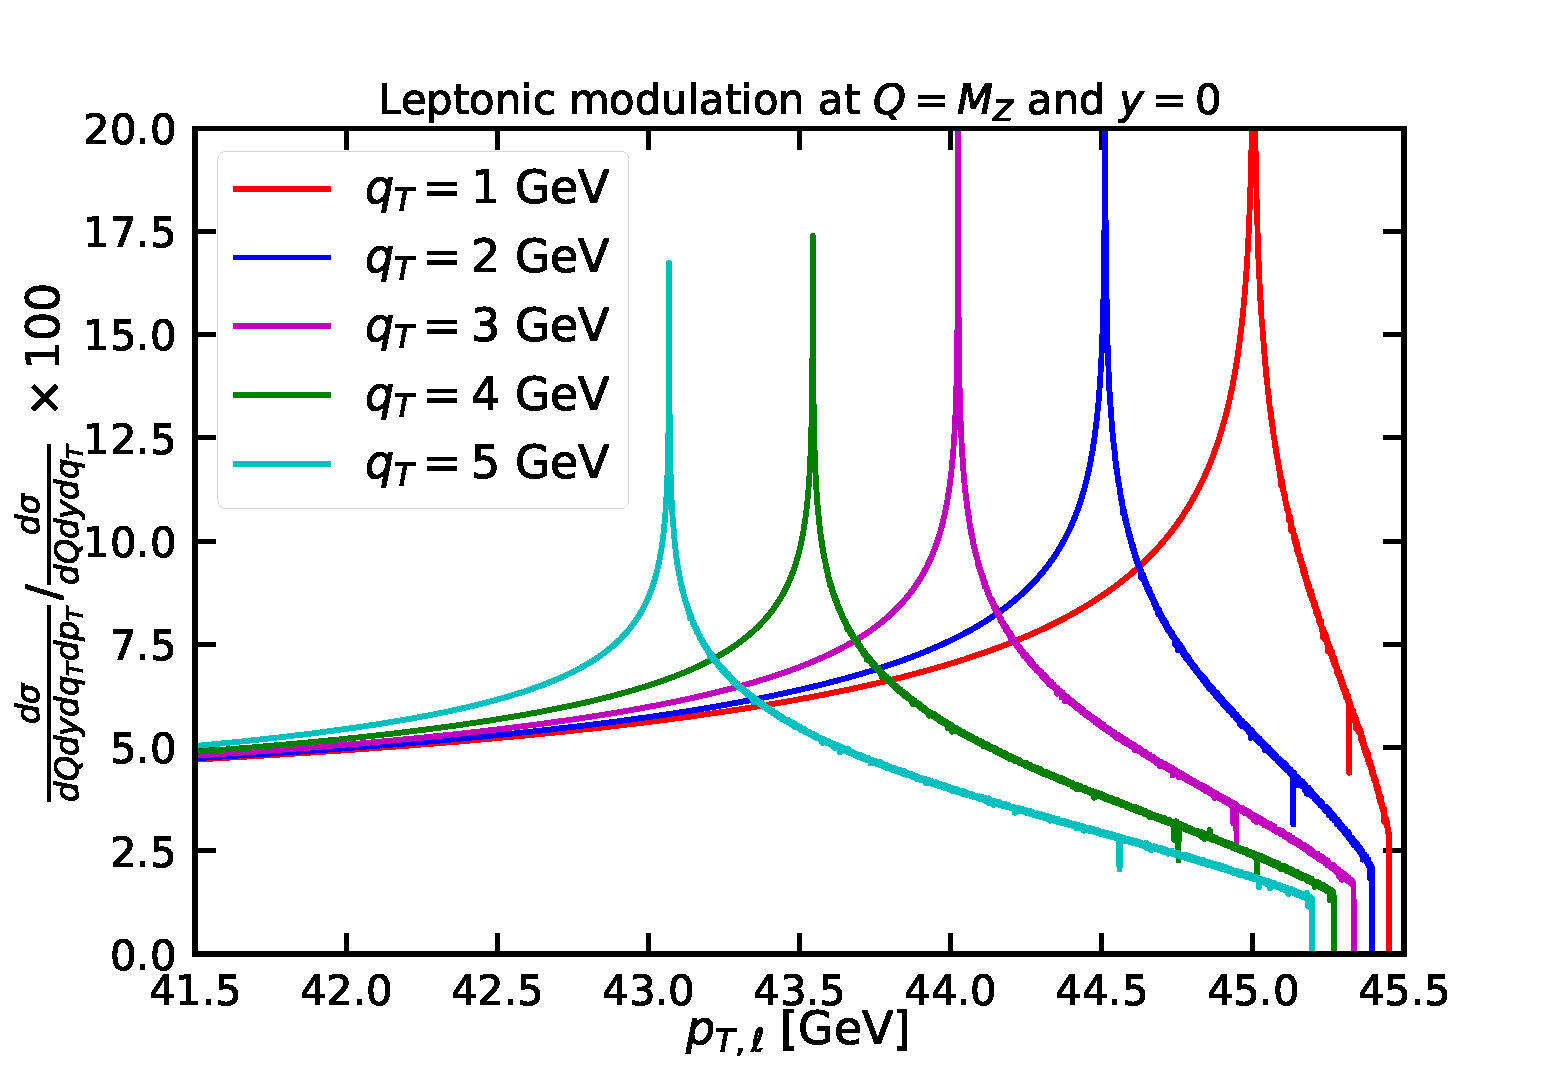
\includegraphics[width=0.8\textwidth]{plots/LeptonicModulation.pdf}
    \caption{Behaviour of the second line of
      Eq.~(\ref{eq:LeptonicModulation}) at $Q=M_Z$ and $y=0$ as a
      function of the lepton transverse momentum
      $p_{T,\ell}$.\label{fig:LeptonicModulation}}
  \end{centering}
\end{figure}

\section{Convolution in transverse-momentum space}

The ``transverse-momentum'' version of Eq.~(\ref{eq:crosssection}) reads:
\begin{equation}\label{eq:crosssectionkt}
\begin{array}{rcl}
  \displaystyle \frac{d\sigma}{dQ dy dq_T} &=&\displaystyle 
  \frac{16\pi\alpha^2q_T}{9 Q^3} H(Q,\mu) \sum_q C_q(Q)\\
\\
&\times&\displaystyle 
  \int d^2\mathbf{k}_{T,1}d^2\mathbf{k}_{T,2}
  \overline{F}_q(x_1,\mathbf{k}_{T,1};\mu,\zeta)
  \overline{F}_{\bar{q}}(x_2,\mathbf{k}_{T,2};\mu,\zeta)\delta^{(2)}(\mathbf{q}_{T}-\mathbf{k}_{T,1}-\mathbf{k}_{T,2})\,,
\end{array}
\end{equation}
where, with abuse of notation, we used the same symbol for the
distributions $F$ both in $k_T$ and $b_T$ space. We can make use of
the $\delta$-function to reduce the expression above to:
\begin{equation}\label{eq:crosssectionkt2}
\frac{d\sigma}{dQ dy dq_T} =\frac{16\pi\alpha^2q_T}{9 Q^3} H(Q,\mu) \sum_q C_q(Q)\int d^2\mathbf{k}_{T}
  \overline{F}_q(x_1,\mathbf{k}_{T};\mu,\zeta)
  \overline{F}_{\bar{q}}(x_2,\mathbf{q}_{T}-\mathbf{k}_{T};\mu,\zeta)\,.
\end{equation}
Since the distributions $F$ only depend on the absolute value of their
argument (be it $k_T$ or $b_T$), the expression above can be further
reduced to:
\begin{equation}\label{eq:crosssectionkt3}
\begin{array}{rcl}
\displaystyle \frac{d\sigma}{dQ dy dq_T} &=&\displaystyle
                                             \frac{16\pi\alpha^2q_T}{9
                                             Q^3} H(Q,\mu) \sum_q
                                             C_q(Q)\\
\\
&\times&\displaystyle \int_0^\infty dk_{T}\,k_{T}\int_0^{2\pi}d\theta\,
  \overline{F}_q(x_1,k_T;\mu,\zeta)
  \overline{F}_{\bar{q}}(x_2,\sqrt{q_{T}^2+k_{T}^2
  -2q_{T}k_{T}\cos\theta};\mu,\zeta)\,,
\end{array}
\end{equation}
where, without loss of generality, we are assuming that the vector
$\mathbf{q}_T$ is directed along the $x$ axis. Knowing the functions
$F$ in $k_T$ space, the formula above can be implemented numerically.

\section{The $A_0$ coefficient}

Using Eq.~(5) of Ref.~\cite{Richter-Was:2016mal}, the azimuthal angle
$\theta$ of the (negative) lepton in the Collins-Soper frame can be
related to the momenta on the vector boson and of one of the leptons
in the laboratory frame as:
\begin{equation}\label{eq:RitterSport}
\cos\theta(\eta,p_T) = \mbox{sign}(y)\frac{2p_T}{Q}\sinh(y-\eta).
\end{equation}
This can be related to the coefficient $A_0$ as~\cite{Gauld:2017tww}:
\begin{equation}
A_0= 4 - 10\,\langle\cos^2\theta\rangle\,,
\end{equation}
where:
\begin{equation}
\begin{array}{rcl}
\displaystyle \langle\cos^2\theta\rangle &\equiv& \displaystyle  \left[\int dp_Td\eta
  \frac{d\sigma}{dQdydq_T d\eta dp_T}\right]^{-1}\int
  dp_Td\eta\left[\cos\theta(\eta, p_T)\right]^2 \frac{d\sigma}{dQdydq_T d\eta dp_T}\,.
\end{array}
\end{equation}
If the integration in both numerator and denominator in the r.h.s. of
the quantity above is performed over the full phase space, the result
at small $q_T$ is:
\begin{equation}
\langle\cos^2\theta\rangle =\int
  dp_Td\eta\left[\cos\theta(\eta, p_T)\right]^2 \frac{d\mathcal{P}}{dp_Td\eta}\,
\end{equation}
with the element of phase space $d\mathcal{P}$ is given in
Eq.~(\ref{eq:difflepphasespace}). Therefore, the ``QCD dynamics''
totally cancels in the ratio and one is left with a relatively
interesting kinematic factor.

\section{Implementing the $\phi*$ distribution}

A physical observable that is particularly useful to probe the
intrinsic transverse dynamics of hadrons is the so-called $\phi^*$
distribution in Drell-Yan production, defined as~\cite{Banfi:2010cf}:
\begin{equation}
\phi^*=\tan\left(\frac{\pi-\Delta\phi}{2}\right)\sin\theta^*=\tan\left(\frac{\pi-\Delta\phi}{2}\right)\sqrt{1-\tanh^2\left(\frac{\Delta\eta}{2}\right)}\,,
\end{equation}
where $\Delta\phi = \phi_1-\phi_2$ and $\Delta\eta = \eta_1-\eta_2$
are the separation in azimuthal angle and pseudo-rapidity of the two
outgoing leptons. The reason why $\phi^*$ is interesting is that
experimental measurements of this quantity reach an extremely high
accuracy. It is therefore useful to express the Drell-Yan cross
section differential in $q_T$ into a cross section differential in
$\phi^*$. This is achieved through the chain rule:
\begin{equation}
\frac{d\sigma}{dQdydq_T d\eta dp_T} = \frac{d\phi^*}{dq_T}\frac{d\sigma}{dQdyd\phi^*d\eta dp_T}\,.
\end{equation}
Of course, this requires the knowledge of $\phi^*$ as a function of
$q_T$ which is what we will work out in the following. The starting
point is the four-momentum conservation $q=p_1+p_2$. Taking the
absolute value
of this relation and using the parameterisations in
Eq.~(\ref{eq:qexplicit}) for $q$ and in Eq.~(\ref{eq:pexplicit}) for
both $p_1$ and $p_2$ immediately gives:
\begin{equation}\label{eq:coshdeta}
\cosh\Delta\eta = 1+\frac{Q^2}{2p_{T1}p_{T2}}\,. 
\end{equation}
In addition, equating the absolute values of the transverse component
($|\mathbf{q}_T|^2=|\mathbf{p}_{T1}+\mathbf{p}_{T2}|^2$) leads to:
\begin{equation}\label{eq:cosdphi}
\cos\Delta\phi =\frac{p_{T1}^2+p_{T2}^2-q_T^2}{2p_{T1}p_{T2}}\,.
\end{equation}
Using Eq.~(\ref{eq:coshdeta}) one has:
\begin{equation}
\tanh\left(\frac{\Delta\eta}{2}\right) =
\sqrt{\frac{\cosh\Delta\eta-1}{\cosh\Delta\eta+1}} = \sqrt{\frac{Q^2}{Q^2+4p_{T1}p_{T2}}}\,,
\end{equation}
so that:
\begin{equation}
\sin\theta^*=\sqrt{1-\tanh^2\left(\frac{\Delta\eta}{2}\right)}
=\sqrt{\frac{4p_{T1}p_{T2}}{Q^2 + 4p_{T1}p_{T2}}}\,.
\end{equation}
On the other hand, using Eq.~(\ref{eq:cosdphi}) one finds:
\begin{equation}
\tan\left(\frac{\pi-\Delta\phi}{2}\right) = \sqrt{\frac{1-\cos(\pi-\Delta\phi)}{1+\cos(\pi-\Delta\phi)}}=\sqrt{\frac{1+\cos\Delta\phi}{1-\cos\Delta\phi}}=\sqrt{\frac{p_{T1}^2+p_{T2}^2-q_T^2+2p_{T1}p_{T2}}{p_{T1}^2+p_{T2}^2-q_T^2-2p_{T1}p_{T2}}}\,.
\end{equation}
Now let us define $p_{T1}=p_T$ and $\eta=\eta_1$ and trade $p_{T2}$
for $\cosh(y-\eta)$ using the relation:
\begin{equation}
p_{T2}^2=M^2+p_T^2-2p_TM\cosh(y-\eta)
\end{equation}
with $M=\sqrt{Q^2+q_T^2}$. This gives:
\begin{equation}
\sin\theta^*=\sqrt{\frac{4p_{T}\sqrt{M^2+p_T^2-2p_TM\cosh(y-\eta)}}{Q^2 +4p_{T}\sqrt{M^2+p_T^2-2p_TM\cosh(y-\eta)}}}\,.
\end{equation}
and:
\begin{equation}
\tan\left(\frac{\pi-\Delta\phi}{2}\right) = \sqrt{\frac{Q^2+2p_T\left[p_T-M\cosh(y-\eta)+\sqrt{M^2+p_T^2-2p_TM\cosh(y-\eta)}\right]}{Q^2+2p_T\left[p_T-M\cosh(y-\eta)-\sqrt{M^2+p_T^2-2p_TM\cosh(y-\eta)}\right]}}\,.
\end{equation}
Gathering all pieces together finally gives:
\begin{equation}\label{eq:phistarmaster}
\begin{array}{rcl}
\phi^*&=&\displaystyle
          \sqrt{\frac{Q^2+2p_T\left[p_T-M\cosh(y-\eta)+\sqrt{M^2+p_T^2-2p_TM\cosh(y-\eta)}\right]}{Q^2+2p_T\left[p_T-M\cosh(y-\eta)-\sqrt{M^2+p_T^2-2p_TM\cosh(y-\eta)}\right]}}\\
\\
&\times& \displaystyle\sqrt{\frac{4p_{T}\sqrt{M^2+p_T^2-2p_TM\cosh(y-\eta)}}{Q^2 +4p_{T}\sqrt{M^2+p_T^2-2p_TM\cosh(y-\eta)}}}\,.
\end{array}
\end{equation}

One can show that the boost required to go from the laboratory frame,
in which the vectors $q$ and $p$ are given by
Eqs.~(\ref{eq:qexplicit}) and~(\ref{eq:pexplicit}), respectively, with
$p_T$ given by Eq.~(\ref{eq:overpT}), to the Collins-Soper frame, in
which:
\begin{equation}\label{eq:CSdecomp}
q = Q(1,0,0,0)\quad\mbox{and}\quad p = \frac{Q}2(1,\sin\theta\cos\phi, \sin\theta\sin\phi,\cos\theta)\,,
\end{equation}
is given by:
\begin{equation}\label{eq:boostLabToCS}
\Lambda_{{\rm Lab}\rightarrow {\rm CS}} = 
\begin{pmatrix}
\frac{M}{Q}\cosh y & -\frac{q_T}{Q} & 0 & -\frac{M}{Q}\sinh y\\
-\frac{q_T}{Q}\cosh y & \frac{M}{Q} & 0 & \frac{q_T}{Q}\sinh y\\
0 & 0 & 1 & 0 \\
-\sinh y & 0 & 0 & \cosh y
\end{pmatrix}\,,
\end{equation}
with $M=\sqrt{Q^2+q_T^2}$. Likewise, the boost to go from the
Collins-Soper to the laboratory frame is the inverse of the above
transformation and reads:
\begin{equation}\label{eq:boostCSToLab}
\Lambda_{ {\rm CS}\rightarrow{\rm Lab}} = \Lambda_{{\rm Lab}\rightarrow {\rm CS}}^{-1}=
\begin{pmatrix}
\frac{M}{Q}\cosh y & \frac{q_T}{Q}\cosh y & 0 & \sinh y\\
\frac{q_T}{Q} & \frac{M}{Q} & 0 & 0\\
0 & 0 & 1 & 0 \\
\frac{M}{Q}\sinh y & \frac{q_T}{Q}\sinh y & 0 & \cosh y
\end{pmatrix}\,.
\end{equation}
Notice that rotating the vector in Eq.~(\ref{eq:pexplicit}) using the
transformation in Eq.~(\ref{eq:boostLabToCS}) and equating the $z$
component to that of the vector $p$ in Eq.~(\ref{eq:CSdecomp})
immediately gives Eq.~(\ref{eq:RitterSport}). This immediately allows
one to write:
\begin{equation}
\sin\theta = \frac{\sqrt{Q^2-4p_T\sinh^2(\eta-y)}}{Q}
\end{equation}

\section{QED radiative corrections to the leptonic final state}

In this section, we will show how to include into the Drell-Yan cross
section the corrections due to QED final-state collinear
radiation. This will be done at LO + (N)LL accuracy which means that
the leptonic tensor will be computed at the first fixed perturbative
order while the collinear radiation will be resummed to the first
(second) logarithmic order.

Assuming massless, unpolarised leptons, considering only collinear
radiation, and concentrating on cross sections integrated over the
polar angle, the leptonic tensor can be generally decomposed into the
following Lorentz structures~\cite{Ebert:2020dfc}:
\begin{equation}
\begin{array}{rcl}
L^{\mu\nu}(q, p_1,p_2) &=&\displaystyle 
\left(-g^{\mu\nu}+\frac{q^\mu
    q^\nu}{Q^2}\right)\mathcal{F}_1(z_1,z_2, Q^2)+\frac{1}{p\cdot
  q}\left(p^{\mu}-\frac{p\cdot
  q}{Q^2}q^{\mu}\right)\left(p^{\nu}-\frac{p\cdot
  q}{Q^2}q^{\nu}\right)\mathcal{F}_2(z_1,z_2, Q^2)\\
\\
&-&\displaystyle
    i\varepsilon^{\mu\nu\rho\sigma}\frac{q_{\rho}p_{\sigma}}{2p\cdot q}\mathcal{F}_3(z_1,z_2, Q^2)\,.
\end{array}
\label{eq:leptonictensor}
\end{equation}
where $p=p_1$, $Q^2=q^2$, $z_i=2p_i\cdot q/Q^2$ with $i=1,2$, and
where the functions $\mathcal{F}$ are purposely reminiscent of the
semi-inclusive DIS structure functions. This structure functions allow
a collinear factorisation in terms of hard cross sections and
collinear fragmentation functions (FFs):
\begin{equation}
\mathcal{F}_S(z_1,z_2,Q^2)=c_S(Q^2)\sum_{i,j=e^\pm,\gamma}\int_{z_1}^1\frac{dy_1}{y_1}\int_{z_2}^1\frac{dy_2}{y_2}C_{ij}^{(S)}\left(\frac{y_1}{z_1},
  \frac{y_2}{z_2},\alpha(Q)\right)d_{i/e^-}(y_1,Q) d_{j/e^+}(y_2,Q)\,,\quad S=1,2,3\,,
\end{equation}
where $c_S$ is the appropriate electroweak charge (that also contains
the vector-boson propagator) with $c_1=c_2$. Therefore, the fully
differential cross section for inclusive Drell-Yan production in
hadronic collisions reads:
\begin{equation}
\frac{d\sigma}{d^4p_1d^4p_2} = \int d^4q\,W_{\mu\nu}(P_1,P_2,q) L^{\mu\nu}(q,p_1,p_2)\,,
\end{equation}
where $W_{\mu\nu}$ is the hadronic tensor and $P_{1,2}$ are the
momenta of the incoming hadrons. Notice that here we are assuming that
there is non interference between in the leptonic and the hadronic
parts. Importantly, one generally has $q\neq p_1+ p_2$ due to possible
radiation that is eventually integrated over into the structure
functions. The differential cross section with respect to the
lepton-pair momentum $\overline{q}=p_1+p_2$ within a certain fiducial
region defined by the function $\Theta(p_1,p_2)$ is computed as:
\begin{equation}
  \frac{d\sigma}{d^4\overline{q}}=\int d^4p_1d^4p_2\left[\int d^4q\,W_{\mu\nu}(P_1,P_2,q) L^{\mu\nu}(q,p_1,p_2)\right]\delta^{(4)}(\overline{q}-p_1-p_2)\Theta(p_1,p_2)\,.
\end{equation}

If no QED radiation, either hard or collinear, is allowed the hard
cross sections reduce to:
\begin{equation}
C_{ij,\rm LO}^{(S)}(y_1,y_2,\alpha(Q))=\delta_{ie^-}\delta_{je^+}\delta(1-y_1) \delta(1-y_2)\,.
\end{equation}
and the relevant FFs to:
\begin{equation}
d_{e^{\pm}/e^\pm}(y,Q)=\delta(1-y)\,.
\end{equation}
such that the structure functions are all equal and become:
\begin{equation}
\mathcal{F}_{S,\rm LO}(z_1,z_2,Q^2)=\delta(1-z_1) \delta(1-z_2) = Q^4\delta(p_2^2) \delta(p_1^2) \theta(p_{1,0}) \theta(p_{2,0})\,.
\end{equation}
Plugging this identity into the leptonic tensor and requiring
$q=p_1+p_2$ (see below), one finds:
\begin{equation}
L^{\mu\nu}(p_1+p_2,p_1,p_2)=Q^2\left[2c_1\left(-g^{\mu\nu}p_1\cdot p_2+p_1^\mu p_2^\nu+p_2^\mu p_1^\nu\right)+ic_3\varepsilon^{\mu\nu\rho\sigma}p_{1\rho}p_{2\sigma}\right]\delta(p_1^2)\delta(p_2^2)\theta(p_{1,0}) \theta(p_{2,0}) \,,
\end{equation}
that is the well-known leptonic tensor multiplied by the on-shell-ness
condition for the leptons. Now the cross section differential in
$q=p_1+p_2$ within a specific set of fiducial cuts on the outgoing
leptons defined by the function $\Theta(p_1,p_2)$ is computed as:
\begin{equation}
  \frac{d\sigma}{d^4q}=\int d^4p_1d^4p_2W_{\mu\nu}(P_1,P_2,q) L^{\mu\nu}(q,p_1,p_2)\delta^{(4)}(q-p_1-p_2)\Theta(p_1,p_2)\,,
\end{equation}
where $W_{\mu\nu}$ is the hadronic tensor. Decomposing the hadronic
tensor in terms of Lorentz structures and taking the contractions with
the leptonic tensor produces the fiducial cross section discussed
above. The Lorentz structure relevant to the unpolaised case is
$g_\perp^{\mu\nu}$ given in Eq.~(\ref{eq:gmunoperp}). Observing the
fact that $g_\perp^{\mu\nu}$ is symmetric, when contracting it with the leptonic tensor in
Eq.~(\ref{eq:leptonictensor}), the term proportional to
$\epsilon^{\mu\nu\rho\sigma}$ automatically drops. We are then left
with:
\begin{equation}
\displaystyle L_\perp(q,p_1,p_2)= g_\perp^{\mu\nu}
    L_{\mu\nu}(q,p_1,p_2) = -2\mathcal{F}_1(z_1,z_2,Q^2)-\frac12z_1\mathcal{F}_2(z_1,z_2,Q^2)+\frac{(zp)^2}{p\cdot
    q}\mathcal{F}_2(z_1,z_2,Q^2)
\end{equation}
where we have used the equalities $z^2=-1$, $t^2=1$, $zq = 0$, and
$p^2=0$.

\newpage
\bibliographystyle{ieeetr}
\bibliography{bibliography}

\end{document}
